% !TeX root = ../main.tex
\documentclass[./../main.tex]{subfiles}

\begin{document}
\section{Phân tích yêu cầu}
Như đã đề cập ở các phần trước, mục tiêu hướng đến của đề tài là xây dựng một phần mềm theo dõi sắn với nhiều tính năng bao gồm xem các bảng dữ liệu về sắn, bệnh trên cây sắn, bản đồ dịch bệnh, chẩn đoán bệnh, xem danh sách nguồn cung, thêm, sửa, xóa các đề xuất thương mại sắn và xem, viết các bài báo. Do đó, hệ thống phải đáp ứng được khả năng quản lý nhiều dữ liệu, cũng như đảm bảo cho cả người dùng và quản trị viên có thể thao tác thuận tiện. Ngoài ra còn có thêm một số chức năng phát triển thêm để phần mềm được hoàn thiện hơn như đăng ký, đăng nhập, quên mật khẩu, chỉnh sửa thông tin cá nhân để người dùng có thể sử dụng với đúng vai trò tương ứng, đảm bảo tính bảo mật, an toàn. Dự án này được phát triển từ bài toán do Viện Khoa học \& Công nghệ Việt Nam - Hàn Quốc (\acrshort{vkist}) đề ra, và nhu cầu thực tiễn của người nông dân trồng sắn hay những người có liên quan đến ngành nông nghiệp này. Vậy nên, việc chú trọng vào \acrshort{ui}/\acrshort{ux} cũng như thiết kế cơ sở dữ liệu sao cho hợp lý, tiết kiệm chi phí là điều cần thiết. Dựa vào những điều trên, sau đây sẽ đi vào phần phân tích vấn đề thành các yêu cầu, các ca sử dụng.

\subsection{Đặc tả yêu cầu chức năng}
% Chia hệ thống thành các nhóm chức năng chính theo mối liên hệ lẫn nhau giữa các chức năng và sự tương đồng trong cách sử dụng, cách thực thi của chúng sẽ thu được các đặc tả yêu cầu của nhóm chức năng. Dựa vào các đặc tả này để phân tích thành các ca sử dụng, đặc tả ca sử dụng và luồng hoạt động. Có thể phân chia đối tượng sử dụng thành 3 nhóm sau: người dùng là khách chỉ có thể xem và tìm kiếm một số thông tin, người dùng có tài khoản đã được xác minh có thể cung cấp nguồn sắn, giao dịch thương mại sắn, viết bài báo mới và cuối cùng là quản trị viên điều hành phần mềm.
Để đáp ứng các yêu cầu về tính dễ dùng, tính bảo mật thông tin của một phần mềm theo dõi sẵn có nhiều tính năng, giúp hỗ trợ người nông dân trong việc tìm hiểu, nắm bắt thông tin về sắn, các đề xuất thương mại sắn, và hỗ trợ cán bộ quản lý dữ liệu liên quan đến sắn, bệnh trên cây,... thì hệ thống cần xây dựng các chức năng sau:

\begin{itemize} 
    \item \textbf{Quản lý tài khoản:} Người dùng khách có thể đăng ký tạo tài khoản. Sau khi tài khoản được quản trị viên duyệt thì có thể dùng tài khoản đó để đăng nhập, sửa lại thông tin cá nhân và các dữ liệu liên quan đến tài khoản đó trên sàn thương mại. Khi muốn kết thúc phiên đăng nhập thì cần đăng xuất khỏi hệ thống.
    \item \textbf{Tổng hợp thông tin về sắn, bệnh trên cây sắn:} Hiển thị tổng hợp các thông tin về sắn, bệnh trên cây sắn dưới dạng bảng giúp người dùng dễ dàng nắm bắt thông tin. Có thể tìm theo tên hoặc nhãn, xem chi tiết thông tin sắn hoặc bệnh trên cây sắn nhằm mục đích tiết kiệm thời gian trong việc tìm kiếm thông tin theo nhu cầu cá nhân.
    \item \textbf{Bản đồ sắn:} Hiển thị bản đồ Tây Ninh với các điểm được đánh dấu nơi diễn ra dịch bệnh và thông tin về dịch bệnh đó. Ngoài ra cũng hỗ trợ người dùng truy vấn thông tin về dịch bệnh theo khu vực, loại bệnh, mức độ nghiêm trọng của dịch bệnh để họ có thể kịp thời ứng phó và tìm cách phòng chống, chữa trị nếu mắc phải.
    \item \textbf{Chẩn đoán bệnh bằng hình ảnh:} Để chẩn đoán bệnh trên cây sắn, người dùng sau khi tải ảnh lên, hệ thống sẽ trả về kết quả xác suất bệnh trên cây sắn được phân tích từ ảnh. Về phần cách để chẩn đoán bệnh, hệ thống sẽ gửi ảnh cho bên thứ ba qua \acrshort{api} và đợi kết quả trả về để hiển thị, nên cách phân tích bệnh qua ảnh sẽ không được trình bày cụ thể trong khóa luận tốt nghiệp này.
    \item \textbf{Danh sách nguồn cung sắn:} Danh sách các tài khoản đã được xác minh và có thể cung cấp nguồn sắn dưới dạng bảng với chức năng có thể tìm kiếm những nhà cung cấp tùy theo yêu cầu người dùng.
    \item \textbf{Thương mại sắn:} Khi đăng nhập vào hệ thống bằng tài khoản đã được xác minh, người dùng có thể theo dõi các hoạt động thương mại về mua, bán sắn, người dùng cũng có thể tham gia tạo đề xuất trao đổi sắn và quản lý các đề xuất đó như thêm giống sắn, gia hạn thêm thời gian giao dịch.
    \item \textbf{Diễn đàn:} Trong khi khách chỉ có thể xem các bài báo công khai trên trang phần mềm, thì người dùng đã được xác minh khi đăng nhập có thể thêm mới các bài viết liên quan đến sắn. Khi đăng bài báo mới, người dùng cần đảm bảo tính đúng đắn và pháp lý, bản quyền của bài báo đó.
    \item \textbf{Quản lý phần mềm đối với quản trị viên:} Quản trị viên có thể quản lý dữ liệu của toàn bộ hệ thống, cụ thể là: dữ liệu về các giống sắn, bệnh trên cây sắn, bản đồ dịch bệnh mà cây sắn mắc phải tại tỉnh Tây Ninh, quản lý diễn đàn sắn, và quản lý tài khoản người dùng, xác minh các tài khoản mới.
\end{itemize}

\subsection{Đặc tả yêu cầu phi chức năng}
Dựa vào bài toán đã được xác định trong phần mở đầu, kết hợp với việc phân tích trải nghiệm người dùng và các tiêu chuẩn dành cho một trang web như tính khả dụng, tính ổn định, tính bảo mật, hiệu năng hoạt động, khả năng bảo trì để đưa ra các yêu cầu phi chức năng. Đây cũng là cơ sở cho việc kiểm thử hệ thống sau này có đáp ứng được các yêu cầu này không, từ đó đưa ra đánh giá và hướng giải quyết.

\subsubsection{Hiệu suất phần mềm}
% Hiệu suất (Usability): Mức độ thân thiện với người dùng (dễ dàng sử dụng).
\begin{enumerate}
    \item Giao diện cần có sự thống nhất về bố cục và thân thiện với người dùng, nội dung được hiển thị trực quan, phù hợp với chủ đề chung của phần mềm, đáp ứng các đối tượng người dùng đã xác định trước đó.
    \item Có thể hiển thị các giao diện, bố cục khác nhau tùy thuộc vào thiết bị điện tử mà người dùng sử dụng, từ máy tính xách tay, máy tính bảng đến các thiết bị nhỏ hơn như điện thoại thông minh, hỗ trợ các trình duyệt web phổ biến như Google Chrome, Microsoft Edge, Samsung Internet,... Để việc trình bày giao diện đạt hiệu quả tốt nhất, khuyến khích người sử dụng dùng trình duyệt Google Chrome trên máy tính xách tay hay máy cây.
\end{enumerate}

\subsubsection{Bảo mật hệ thống}
\begin{enumerate}
    \item Đảm bảo phân quyền cho các đối tượng đúng thẩm quyền, giới hạn các chức năng có thể sử dụng ở cả frontend và backend theo đối tượng sử dụng. Nhờ đó, các tác nhân sẽ chỉ có thể và chỉ tập trung vào các chức năng mà họ có thể sử dụng, tránh việc nhầm lẫn có thể ảnh hưởng tới dữ liệu hệ thống.
    \item Một số chức năng đặc thù dành riêng có người dùng có tài khoản đã xác minh như quản lý đề xuất sắn và viết bài báo mới, đều sẽ tác động đến cơ sở dữ liệu, đều cần phải thông qua tài khoản đã đăng nhập và gửi yêu cầu bằng token còn hiệu lực. Từ đó tránh được việc tạo ra các thông tin giả, gây nhiễu loạn thông tin cho người dùng khác. Việc xác minh tài khoản cũng giúp cho quản trị viên có thể liên lạc tới người dùng trong trường hợp gặp sự cố.
\end{enumerate}

\subsubsection{Hiệu năng hoạt động}
% Hiệu quả hoạt động (Performance Efficiency): Hiệu suất mà phần mềm hệ thống phản hồi tại 1 thời điểm. Ví dụ như khi hệ thống đạt mức sử dụng cao nhất hoặc thấp nhất.
Phần mềm cần hoạt động liên tục, hạn chế thời gian chết trong quá trình cài đặt phần mềm trên máy chủ ảo, đảm bảo đáp ứng được các yêu cầu từ người dùng lên tới 100 người dùng cùng lúc và thời gian phản hồi là dưới 1 giây.

\subsubsection{Khả năng bảo trì}
% Khả năng bảo trì (Maintainability): Tính dễ dàng thay đổi, sửa lỗi để cải thiện hiệu suất, hoặc để tương thích với môi trường mới.
\begin{enumerate}
    \item Cần sao lưu dữ liệu của hệ thống phòng trường hợp các sự cố như bị tấn công, hay máy chủ gặp vấn đề gây mất mát dữ liệu, từ đó nhanh chóng phục hồi dữ liệu và tiếp tục vận hành hệ thống. Nếu gặp vấn đề trong phiên bản mới vừa cập nhật trên máy chủ, cần phải đảm bảo có thể quay trở lại phiên bản trước và sửa lỗi kịp thời, tránh làm ảnh hưởng tới việc sử dụng phần mềm.
    \item Phần mềm có thể dễ dàng cài đặt và quản lý bằng việc ứng dụng Github trong quản lý các phiên bản phần mềm và Docker compose trong việc cài đặt hệ thống. Vậy nên có thể di chuyển sản phẩm sang những môi trường, hệ điều hành khác mà vẫn đảm bảo tính nhất quán, ổn định.
\end{enumerate}

\subsubsection{Khả năng phát triển}
% Khả năng phát triển (Extensibility): Đo mức độ có thể phát triển tính năng mới trong tương lai hay không.
Khi đã có được lượng người dùng cố định, thì việc hệ thống cần phải phát triển thêm các tính năng mới, mở rộng quy mô, đáp ứng nhu cầu phát sinh của người dùng là điều cần thiết,  nhờ đó không chỉ đảm bảo số lượng người đang sử dụng, mà còn có thể thu hút thêm người dùng tiềm năng.

\section{Đặc tả các ca sử dụng}
\subsection{Tổng quan}

Từ các phân tích trên, đối tượng sử dụng sẽ được chia thành 3 tác nhân theo nhóm các chức năng mà mỗi tác nhân có thể sử dụng.
\begin{figure}[H]
    \centering
    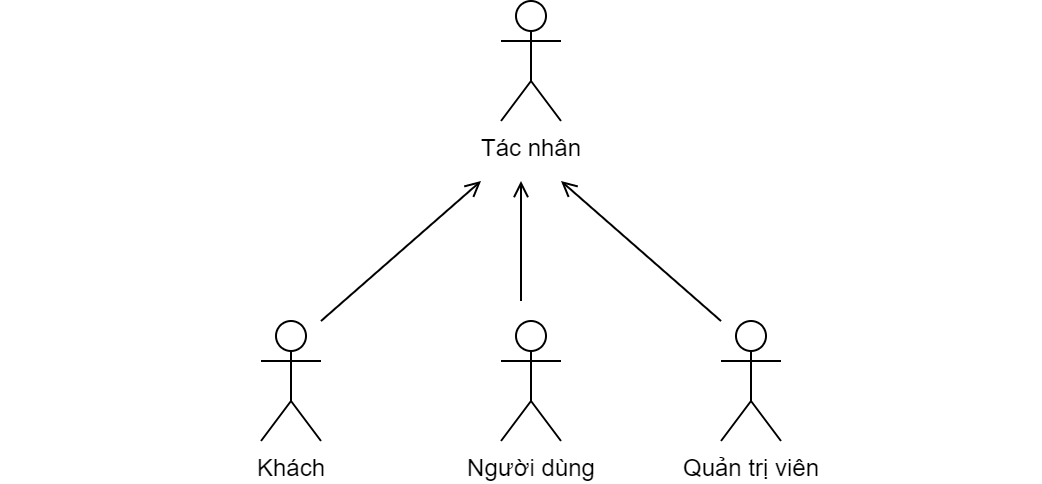
\includegraphics[width=\linewidth]{./img/actors.png}
    \caption{Các tác nhân hệ thống}
\end{figure}

Hệ thống có 3 tác nhân:
\begin{itemize}
    \item \textbf{Khách}: Bất kỳ người dùng nào khi truy cập website đều có thể xem và tra cứu các thông tin mở. Nhóm người này có thể xem và tìm kiếm các thông tin hữu ích liên quan đến sắn.
    \item \textbf{Người dùng}: Người dùng của hệ thống cần phải có tài khoản đã xác nhận. Nhóm người này có thể truy cập vào website và thực hiện các công việc yêu cầu tính xác minh thông tin cá nhân, vậy nên cần phải cung cấp đủ thông tin cũng như cần được quản trị viên duyệt. Một số công việc mà Người dùng có thể thực hiện: thao tác thêm, sửa, xóa đề xuất trên trang thương mại sắn, cập nhật thông tin người dùng,...
    \item \textbf{Quản trị viên}: Người quản trị toàn bộ cơ sở dữ liệu của hệ thống và Người dùng. Đồng thời cũng là người cập nhật cơ sở dữ liệu, giải quyết các vấn đề của hệ thống. Nhóm người này có thể  là quản trị hệ thống cả về nội dung và con người để đảm bảo hệ thống diễn ra ổn định. Người dùng cần phải được Quản trị viên xác nhận tài khoản để chính thức trở thành Người dùng.
\end{itemize}

Hình dưới đây sẽ tổng hợp lại các ca sử dụng có trong hệ thống.

\begin{figure}[H]
    \centering
    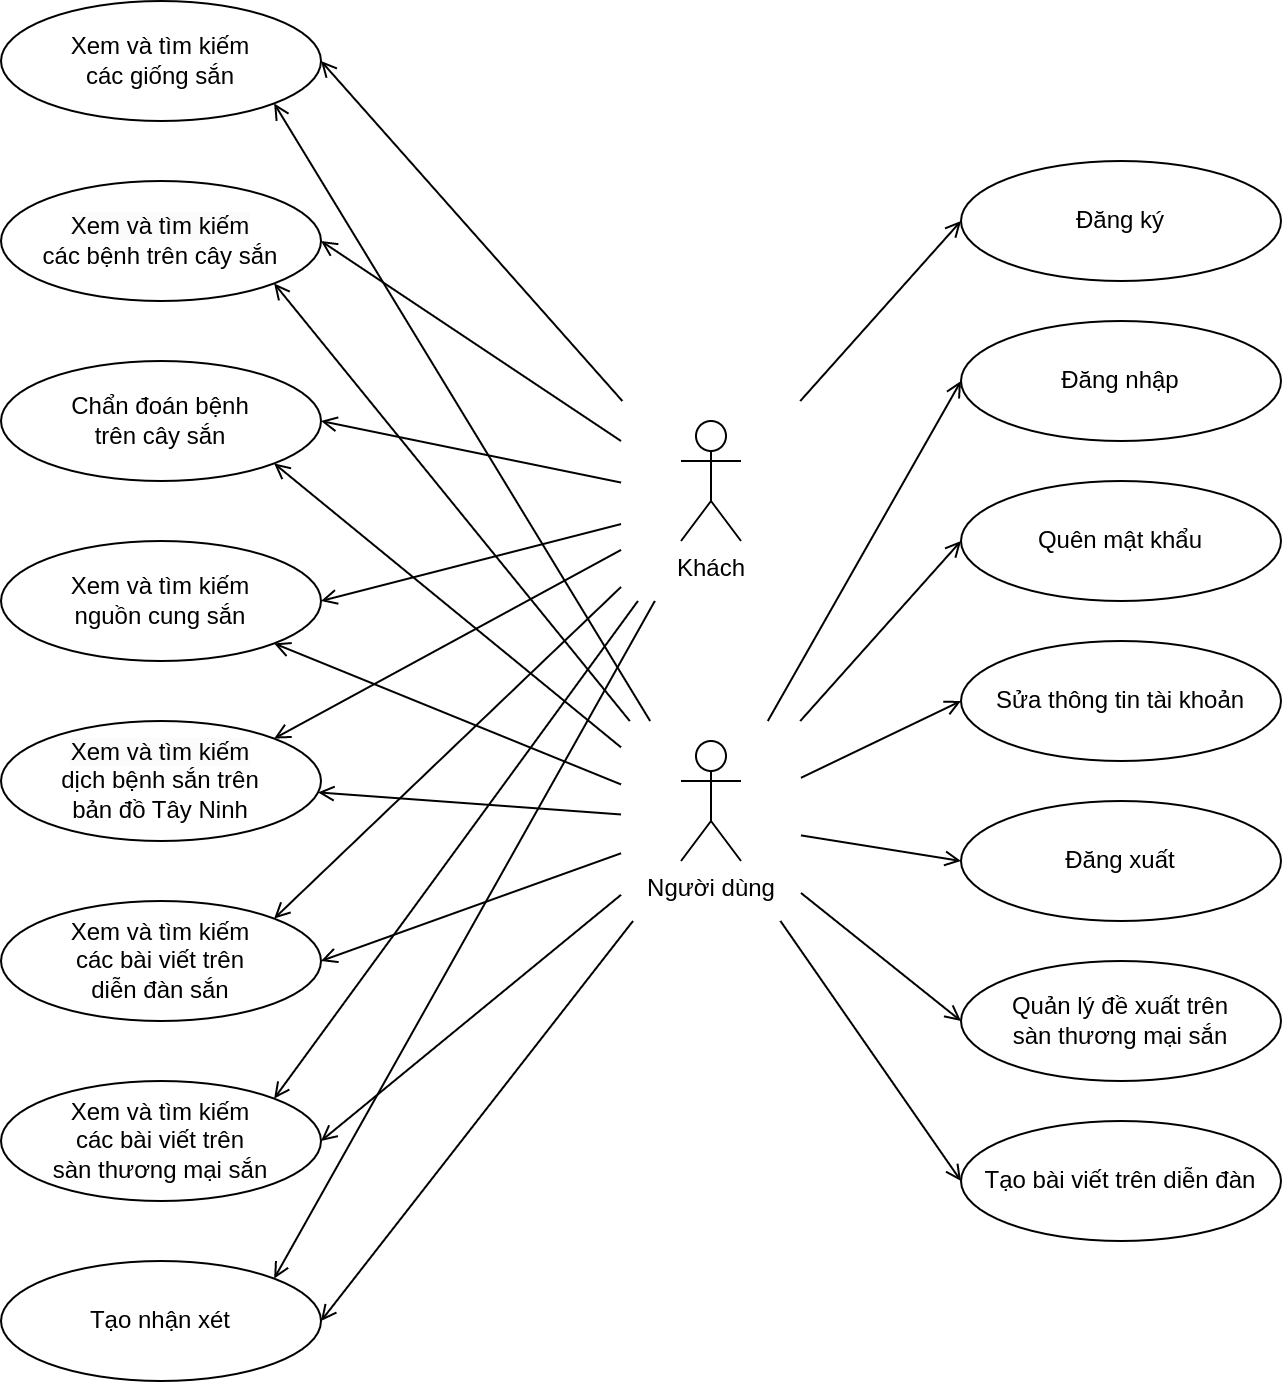
\includegraphics[height=\linewidth]{./img/uc-g-u.png}
    \caption{Biểu đồ các ca sử dụng của khách và người dùng}
\end{figure}

\begin{figure}[H]
    \centering
    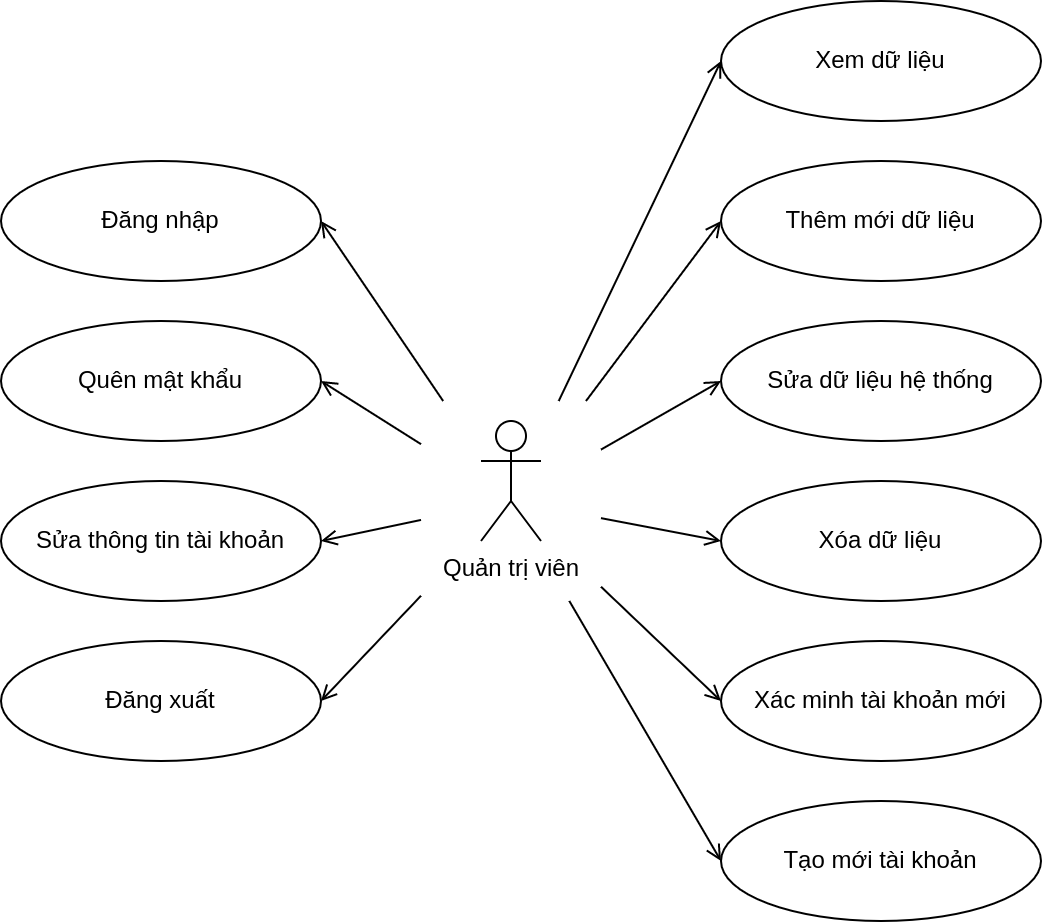
\includegraphics[height=0.6\linewidth]{./img/uc-admin.png}
    \caption{Biểu đồ các ca sử dụng của quản trị viên}
\end{figure}

Tương ứng với mỗi tác nhân sẽ có các ca sử dụng sau:
\begin{itemize}
    \item \textbf{Các ca sử dụng của tác nhân Khách}: xem và tìm kiếm các giống sắn, xem và tìm kiếm các bệnh trên cây sắn, chẩn đoán bệnh trên cây sắn, xem và tìm kiếm nguồn cung sắn, xem và tìm kiếm dịch bệnh sắn trên bản đồ Tây Ninh, xem và tìm kiếm các bài viết trên diễn đàn sắn, xem và tìm kiếm các bài viết trên sàn thương mại sắn, tạo nhận xét, đăng ký.
    \item \textbf{Các ca sử dụng của tác nhân Người dùng}: xem và tìm kiếm các giống sắn, xem và tìm kiếm các bệnh trên cây sắn, chẩn đoán bệnh trên cây sắn, xem và tìm kiếm nguồn cung sắn, xem và tìm kiếm dịch bệnh sắn trên bản đồ Tây Ninh, xem và tìm kiếm các bài viết trên diễn đàn sắn, xem và tìm kiếm các bài viết trên sàn thương mại sắn, tạo nhận xét, đăng nhập, quên mật khẩu, sửa thông tin tài khoản, đăng xuất, quản lý đề xuất trên sàn thương mại sắn, tạo bài viết trên diễn đàn.
    \item \textbf{Các ca sử dụng của tác nhân Quản trị viên}: đăng nhập, quên mật khẩu, sửa thông tin tài khoản, đăng xuất, xem dữ liệu của hệ thống, thêm mới dữ liệu vào cơ sở dữ liệu, sửa dữ liệu hệ thống, xóa dữ liệu trong cơ sở dữ liệu, xác minh tài khoản mới, tạo mới tài khoản.
\end{itemize}

Để làm rõ hơn các chức năng của hệ thống, phần tiếp theo sẽ trình bày chi tiết các ca sử dụng. Trong mỗi phần sẽ bao gồm mô tả ngắn gọn về ca sử dụng, tác nhân có thể thực hiện, luồng cơ bản, các luồng thay thế, tiền điều kiện, và hậu điều kiện.

\subsection{Ca sử dụng Đăng ký}
\begin{itemize}
    \item \textbf{Mô tả}: Khách đăng ký làm người dùng của hệ thống.
    \item \textbf{Tác nhân}: Khách
    \item \textbf{Luồng cơ bản}:
    \begin{table}[H]
    \caption{\label{uc-1}Luồng cơ bản trong ca sử dụng đăng ký}
    \begin{tabularx}{\textwidth}{| X | X | X |}
        \hline
        \textbf{Hành động} & \textbf{Phản hồi hệ thống} & \textbf{Dữ liệu} \\ \hline
        Khách vào trang Đăng nhập và chọn Yêu cầu tạo tài khoản. & Hệ thống hiển thị biểu mẫu đăng ký bao gồm các trường thông tin: email, mật khẩu, nhập lại mật khẩu, tài khoản, họ và tên, số điện thoại. &
        \\ \hline
        Khách nhập đúng và đủ các trường thông tin cần thiết rồi nhấn nút Gửi yêu cầu. & Hệ thống ghi nhận các biểu mẫu hợp lệ và thông báo kết quả Đã gửi yêu cầu thành công & Nếu thông tin không chính xác thì thực hiện luồng thay thế. Nếu chính xác thì tiếp tục luồng cơ bản.
        \\ \hline
        & Hệ thống cập nhật thông tin của khách đã gửi yêu cầu tạo tài khoản vào hàng đợi chờ Quản trị viên duyệt. & Thông tin đăng ký được lưu vào cơ sở dữ liệu.
        \\ \hline
    \end{tabularx}
    \end{table}
    \item \textbf{Luồng thay thế}:
    \begin{table}[H]
    \caption{\label{uc-2}Luồng thay thế thông tin không hợp lệ trong ca sử dụng đăng ký}
    \begin{tabularx}{\textwidth}{| X | X | X |}
        \hline
        \textbf{Hành động} & \textbf{Phản hồi hệ thống} & \textbf{Dữ liệu} \\ \hline
        Biểu mẫu người dùng nhập không hợp lệ. & Hệ thống cảnh báo trường thông tin không chính xác bằng cách bôi đỏ trường và hiện gợi ý sửa. & Dữ liệu không chính xác.
        \\ \hline
        & Hệ thống yêu cầu khách điền lại dữ liệu. & Dữ liệu không chính xác.
        \\ \hline
        Người dùng đồng ý sửa, điền thêm thông tin. & Quay về luồng cơ bản ở bước tương ứng. & Thông tin đăng ký đã được thay đổi.
        \\ \hline
        Người dùng không đồng ý sửa, điền thêm thông tin. & Đóng biểu mẫu và kết thúc ca sử dụng. & 
        \\ \hline
    \end{tabularx}
    \end{table}    
    \begin{table}[H]
    \caption{\label{uc-3}Luồng thay thế làm mới biểu mẫu trong ca sử dụng đăng ký}
    \begin{tabularx}{\textwidth}{| X | X | X |}
        \hline
        \textbf{Hành động} & \textbf{Phản hồi hệ thống} & \textbf{Dữ liệu} \\ \hline
        Người dùng chọn Làm mới trên biểu mẫu đăng ký. & Hệ thống xóa hết thông tin đã nhập trên biểu mẫu đăng ký. & Dữ liệu đã nhập bị xóa.
        \\ \hline
    \end{tabularx}
    \end{table}    
    \item \textbf{Tiền điều kiện}: Không trong trạng thái đã đăng nhập.
    \item \textbf{Hậu điều kiện}: Biểu mẫu yêu cầu tạo tài khoản được thêm vào hàng đợi duyệt.
\end{itemize}

\subsection{Ca sử dụng Đăng nhập}
\begin{itemize}
    \item \textbf{Mô tả}: Khách đăng nhập thành người dùng của hệ thống.
    \item \textbf{Tác nhân}: Khách
    \item \textbf{Luồng cơ bản}:
    \begin{table}[H]
    \caption{\label{uc-4}Luồng cơ bản trong ca sử dụng đăng nhập}
    \begin{tabularx}{\textwidth}{| X | X | X |}
        \hline
        \textbf{Hành động} & \textbf{Phản hồi hệ thống} & \textbf{Dữ liệu} \\ \hline
        Khách vào trang Đăng nhập. & Hệ thống hiển thị biểu mẫu đăng nhập bao gồm hai trường email và mật khẩu. &
        \\ \hline
        Khách nhập đúng và đủ các trường thông tin cần thiết rồi nhấn nút Gửi yêu cầu. & Hệ thống ghi nhận các biểu mẫu hợp lệ và thông báo kết quả Đã gửi yêu cầu thành công. & Nếu thông tin không chính xác thì thực hiện luồng thay thế. Nếu chính xác thì tiếp tục luồng cơ bản.
        \\ \hline
        & Hệ thống thông báo đăng nhập thành công, khách trở thành người dùng. & Token được cấp cho người dùng để xác thực các yêu cầu sau này.
        \\ \hline
    \end{tabularx}
    \end{table}    
    \item \textbf{Luồng thay thế}:
        \begin{table}[H]
        \caption{\label{uc-5}Luồng thay thế dữ liệu không hợp lệ trong ca sử dụng đăng nhập}
        \begin{tabularx}{\textwidth}{| X | X | X |}
            \hline
            \textbf{Hành động} & \textbf{Phản hồi hệ thống} & \textbf{Dữ liệu} \\ \hline
            Biểu mẫu người dùng nhập không hợp lệ. & Hệ thống cảnh báo trường thông tin không chính xác bằng cách bôi đỏ trường và hiện gợi ý sửa. & Dữ liệu không hợp lệ.
            \\ \hline
            & Hệ thống yêu cầu khách điền lại dữ liệu. & Dữ liệu không hợp lệ
            \\ \hline
            Người dùng đồng ý sửa, điền thêm thông tin. & Quay về luồng cơ bản ở bước tương ứng. & Dữ liệu đã được sửa để hợp lệ.
            \\ \hline
            Người dùng không đồng ý sửa, điền thêm thông tin. & Đóng biểu mẫu và kết thúc ca sử dụng. & 
            \\ \hline
        \end{tabularx}
        \end{table}  
        \begin{table}[H]
        \caption{\label{uc-6}Luồng thay thế sai thông tin xác thực trong ca sử dụng đăng nhập}
        \begin{tabularx}{\textwidth}{| X | X | X |}
            \hline
            \textbf{Hành động} & \textbf{Phản hồi hệ thống} & \textbf{Dữ liệu} \\ \hline
            Người dùng nhập sai thông tin xác thực. & Hệ thống thông báo xác thực email và mật khẩu không thành công. & Dữ liệu xác thực không chính xác.
            \\ \hline
            & Hệ thống yêu cầu khách điền lại dữ liệu. & Thông tin xác thực sai.
            \\ \hline
            Người dùng đồng ý sửa. & Quay về luồng cơ bản ở bước tương ứng. & Thông tin xác thực đã được sửa.
            \\ \hline
            Người dùng không đồng ý sửa. & Đóng biểu mẫu và kết thúc ca sử dụng. & 
            \\ \hline
        \end{tabularx}
        \end{table}  
    \item \textbf{Tiền điều kiện}:
        \begin{itemize}
            \item{Không trong trạng thái đã đăng nhập.\\}
            \item{Đã gửi yêu cầu tạo tài khoản.}
        \end{itemize}
    \item \textbf{Hậu điều kiện}: Khách đăng nhập thành công thành người dùng hệ thống.
\end{itemize}

\subsection{Ca sử dụng Quên mật khẩu}
\begin{itemize}
    \item \textbf{Mô tả}: Người dùng quên mật khẩu đăng nhập.
    \item \textbf{Tác nhân}: Người dùng
    \item \textbf{Luồng cơ bản}:
    \begin{table}[H]
    \caption{\label{uc-7}Luồng cơ bản trong ca sử dụng quên mật khẩu}
    \begin{tabularx}{\textwidth}{| X | X | X |}
        \hline
        \textbf{Hành động} & \textbf{Phản hồi hệ thống} & \textbf{Dữ liệu} \\ \hline
        Người dùng vào trang Đăng nhập và bấm chọn Quên mật khẩu. & Hệ thống hiển thị biểu mẫu quên mật khẩu gồm duy nhất trường email. &
        \\ \hline
        Người dùng nhập email đã đăng ký với hệ thống và bấm nút Gửi. & Hệ thống ghi nhận yêu cầu và gửi thư điện tử đến email trên. & Nếu email không hợp lệ hoặc email chưa có tài khoản tương ứng thì thực hiện luồng thay thế. Nếu chính xác thì tiếp tục luồng cơ bản.
        \\ \hline
        & Hệ thống thông báo đã gửi thư thành công. &
        \\ \hline
        Người dùng kiểm tra thư điện tử và nhấp vào liên kết được gửi qua mail để được điều hướng đến trang web. & Hệ thống hiển thị biểu mẫu đổi mật khẩu gồm hai trường mật khẩu và nhập lại mật khẩu. &
        \\ \hline
        Người dùng nhập mật khẩu mới theo biểu mẫu và chọn Cập nhật mật khẩu để tiếp tục còn chọn Về trang chủ sẽ thực hiện luồng thay thế. & Khi mật khẩu thay đổi thành công, hệ thống sẽ thông báo cập nhật thành công tới người dùng và kết thúc ca sử dụng. & Mật khẩu không hợp lệ sẽ thực hiện luồng thay thế, nếu hợp lệ sẽ tiếp tục luồng cơ bản.
        \\ \hline
    \end{tabularx}
    \end{table}    
    \item \textbf{Luồng thay thế}:
        \begin{table}[H]
        \caption{\label{uc-8}Luồng thay thế dữ liệu không hợp lệ trong ca sử dụng quên mật khẩu}
        \begin{tabularx}{\textwidth}{| X | X | X |}
            \hline
            \textbf{Hành động} & \textbf{Phản hồi hệ thống} & \textbf{Dữ liệu} \\ \hline
            Biểu mẫu người dùng nhập không hợp lệ. & Hệ thống cảnh báo trường thông tin không hợp lệ bằng thông báo hoặc bôi đỏ trường và hiện gợi ý sửa. & Dữ liệu không hợp lệ.
            \\ \hline
            & Hệ thống yêu cầu người dùng điền lại dữ liệu. & Dữ liệu nhập không hợp lệ.
            \\ \hline
            Người dùng đồng ý sửa, điền thêm thông tin. & Quay về luồng cơ bản ở bước tương ứng. & Dữ liệu đã được nhập lại để hợp lệ.
            \\ \hline
            Người dùng không đồng ý sửa, điền thêm thông tin. & Đóng biểu mẫu và kết thúc ca sử dụng. & 
            \\ \hline
        \end{tabularx}
        \end{table}  
        \begin{table}[H]
        \caption{\label{uc-9}Luồng thay thế email chưa tạo tài khoản trong ca sử dụng quên mật khẩu}
        \begin{tabularx}{\textwidth}{| X | X | X |}
            \hline
            \textbf{Hành động} & \textbf{Phản hồi hệ thống} & \textbf{Dữ liệu} \\ \hline
            Người dùng nhập đúng định dạng email nhưng email chưa được tạo tài khoản. & Hệ thống cảnh báo email đã nhập chưa tồn tại trong hệ thống, lỗi gửi yêu cầu. & Email đúng định dạng nhưng không tồn tại trong hệ thống.
            \\ \hline
            & Hệ thống yêu cầu người dùng điền lại dữ liệu. & Email không tồn tại trong cơ sở dữ liệu.
            \\ \hline
            Người dùng đồng ý sửa. & Quay về luồng cơ bản ở bước tương ứng. & Dữ liệu đã được sửa lại.
            \\ \hline
            Người dùng không đồng ý sửa. & Đóng biểu mẫu và kết thúc ca sử dụng. & 
            \\ \hline
        \end{tabularx}
        \end{table}
        \begin{table}[H]
        \caption{\label{uc-10}Luồng thay thế chọn về trang chủ trong ca sử dụng quên mật khẩu}
        \begin{tabularx}{\textwidth}{| X | X | X |}
            \hline
            \textbf{Hành động} & \textbf{Phản hồi hệ thống} & \textbf{Dữ liệu} \\ \hline
            Người dùng chọn Về trang chủ tại biểu mẫu Thay đổi mật khẩu. & Hệ thống đưa người dùng về trang chủ, kết thúc ca sử dụng. & Dữ liệu đã nhập ở biểu mẫu bị xóa.
            \\ \hline
        \end{tabularx}
        \end{table}
    \item \textbf{Tiền điều kiện}:
        \begin{itemize}
            \item{Không trong trạng thái đã đăng nhập.\\}
            \item{Đã có tài khoản.}
        \end{itemize}
    \item \textbf{Hậu điều kiện}: Người dùng đổi mật khẩu thành công.
\end{itemize}

\subsection{Ca sử dụng Sửa thông tin tài khoản}
\begin{itemize}
    \item \textbf{Mô tả}: Người dùng muốn thay đổi thông tin tài khoản.
    \item \textbf{Tác nhân}: Người dùng
    \item \textbf{Luồng cơ bản}:
    \begin{table}[H]
    \caption{\label{uc-11}Luồng cơ bản trong ca sử dụng sửa thông tin tài khoản}
    \begin{tabularx}{\textwidth}{| X | X | X |}
        \hline
        \textbf{Hành động} & \textbf{Phản hồi hệ thống} & \textbf{Dữ liệu} \\ \hline
        Người dùng vào trang Cá nhân. & Hệ thống hiển thị Biểu mẫu đã được khóa, gồm các trường thông tin bao gồm họ và tên, số điện thoại, email, tài khoản, địa chỉ, các giống sắn đang cung cấp, các giống sắn ngừng cung cấp, thông tin chi tiết, mật khẩu mới, nhập lại mật khẩu mới trong trường hợp muốn thay đổi mật khẩu. &
        \\ \hline
        Người dùng chọn chỉnh sửa trang cá nhân. & Hệ thống mở khóa biểu mẫu để có thể tương tác. & Thông tin hiện tại của tài khoản.
        \\ \hline
        Người dùng điền các thông tin muốn sửa và bấm Lưu thay đổi để tiếp tục luồng cơ bản hoặc Hủy thay đổi để thực hiện luồng thay thế. & Hệ thống thông báo cập nhật thành công và kết thúc ca sử dụng. & Dữ liệu nhập vào không hợp lệ sẽ thực hiện luồng thay thế, nếu hợp lệ thì tiếp tục luồng cơ bản.
        \\ \hline
    \end{tabularx}
    \end{table}    
    \item \textbf{Luồng thay thế}:
        \begin{table}[H]
        \caption{\label{uc-12}Luồng thay thế dữ liệu không hợp lệ trong ca sử dụng sửa thông tin tài khoản}
        \begin{tabularx}{\textwidth}{| X | X | X |}
            \hline
            \textbf{Hành động} & \textbf{Phản hồi hệ thống} & \textbf{Dữ liệu} \\ \hline
            Biểu mẫu người dùng nhập không hợp lệ. & Hệ thống cảnh báo trường thông tin không hợp lệ bằng thông báo hoặc bôi đỏ trường và hiện gợi ý sửa. & Dữ liệu không hợp lệ.
            \\ \hline
            & Hệ thống yêu cầu người dùng điền lại dữ liệu. & Dữ liệu không hợp lệ.
            \\ \hline
            Người dùng đồng ý sửa, điền thêm thông tin. & Quay về luồng cơ bản ở bước tương ứng. & Dữ liệu đã được thay đổi để hợp lệ.
            \\ \hline
            Người dùng không đồng ý sửa, chọn Hủy thay đổi để chuyển sang luồng thay thế hủy thay đổi. & &
            \\ \hline
        \end{tabularx}
        \end{table}  
        \begin{table}[H]
        \caption{\label{uc-13}Luồng thay thế hủy thay đổi trong ca sử dụng sửa thông tin tài khoản}
        \begin{tabularx}{\textwidth}{| X | X | X |}
            \hline
            \textbf{Hành động} & \textbf{Phản hồi hệ thống} & \textbf{Dữ liệu} \\ \hline
            Người dùng chọn hủy thay đổi tại biểu mẫu sửa thông tin tài khoản. & Hệ thống khóa biểu mẫu, kết thúc ca sử dụng. & Dữ liệu được đưa về trạng thái trước khi sửa.
            \\ \hline
        \end{tabularx}
        \end{table}
    \item \textbf{Tiền điều kiện}: Người dùng đã được xác thực đã đăng nhập.
    \item \textbf{Hậu điều kiện}: Người dùng cập nhật thông tin thành công.
\end{itemize}

\subsection{Ca sử dụng Đăng xuất}
\begin{itemize}
    \item \textbf{Mô tả}: Người dùng muốn đăng xuất khỏi hệ thống.
    \item \textbf{Tác nhân}: Người dùng
    \item \textbf{Luồng cơ bản}:
    \begin{table}[H]
    \caption{\label{uc-14}Luồng cơ bản trong ca sử dụng đăng xuất}
    \begin{tabularx}{\textwidth}{| X | X | X |}
        \hline
        \textbf{Hành động} & \textbf{Phản hồi hệ thống} & \textbf{Dữ liệu} \\ \hline
        Người dùng di chuột vào tùy chọn Tài khoản trên thanh điều hướng. & Hệ thống hiển thị danh sách các tùy chọn. &
        \\ \hline
        Người dùng chọn tùy chọn Đăng xuất ở bảng chọn xuất hiện. & Hệ thống thực hiện đăng xuất, đăng xuất thất bại sẽ chuyển sang luồng thay thế, thành công sẽ tiếp tục luồng cơ bản. &
        \\ \hline
        Người dùng trở thành khách, kết thúc ca sử dụng. & Hệ thống hiện thông báo đăng xuất thành công. &
        \\ \hline
    \end{tabularx}
    \end{table}    
    \item \textbf{Luồng thay thế}:
        \begin{table}[H]
        \caption{\label{uc-15}Luồng thay thế đăng xuất thất bại trong ca sử dụng đăng xuất}
        \begin{tabularx}{\textwidth}{| X | X | X |}
            \hline
            \textbf{Hành động} & \textbf{Phản hồi hệ thống} & \textbf{Dữ liệu} \\ \hline
            Người dùng đăng xuất thất bại. & Hệ thống báo lỗi. &
            \\ \hline
            Người dùng đăng xuất lại sẽ chuyển sang luồng cơ bản hoặc kết thúc ca sử dụng. &  &
            \\ \hline
        \end{tabularx}
        \end{table}  
    \item \textbf{Tiền điều kiện}: Người dùng đã đăng nhập hệ thống.
    \item \textbf{Hậu điều kiện}: Người dùng đăng xuất khỏi hệ thống, trở thành khách.
\end{itemize}

\subsection{Ca sử dụng Xem và tìm kiếm các giống sắn}
\begin{itemize}
    \item \textbf{Mô tả}: Các tác nhân xem thông tin tổng hợp, chi tiết về các giống sắn, tìm kiếm giống sắn theo tên, nhãn, tên gốc, tên loài, họ sắn.
    \item \textbf{Tác nhân}: Khách, người dùng.
    \item \textbf{Luồng cơ bản}:
    \begin{table}[H]
    \caption{\label{uc-16}Luồng cơ bản trong ca sử dụng xem và tìm kiếm các giống sắn}
    \begin{tabularx}{\textwidth}{| X | X | X |}
        \hline
        \textbf{Hành động} & \textbf{Phản hồi hệ thống} & \textbf{Dữ liệu} \\ \hline
        Tác nhân vào trang các giống sắn. & Hệ thống hiển thị dữ liệu dưới dạng bảng các thông tin: số thứ tự, nhãn, tên gốc, tên chủng giông, năm phát hành, nòi giống, và cột xem chi tiết. & Dữ liệu về các giống sắn.
        \\ \hline
        Tác nhân chọn xem chi tiết để được chuyển tới trang xem đầy đủ thông tin. & Hệ thống hiển thị thông tin chi tiết về giống sắn, bao gồm cả hình ảnh về loại sắn tương ứng. & Dữ liệu chi tiết về giống sắn tác nhân chọn.
        \\ \hline
        Tác nhân nhập từ khóa vào ô tìm kiếm rồi chọn tìm kiếm khi muốn tìm kiếm giống sắn. & Hệ thống hiển thị danh sách các giống sắn phù hợp với từ khóa, sẽ không hiển thị gì nếu không có kết quả phù hợp. & Dữ liệu các giống sắn phù hợp với từ khóa.
        \\ \hline
        Tác nhân chọn điều hướng trang. & Hệ thống hiển thị danh sách các giống sắn theo điều hướng trang mà tác nhân chọn. & Giá trị điều hướng trang mà tác nhân chọn.
        \\ \hline
        Tác nhân kết thúc ca sử dụng hoặc lặp lại các bước trên nếu muốn tiếp tục tìm kiếm. & &
        \\ \hline
    \end{tabularx}
    \end{table}    
    \item \textbf{Luồng thay thế}:
        \begin{table}[H]
        \caption{\label{uc-17}Luồng thay thế tải lại giống sắn trong ca sử dụng xem và tìm kiếm các giống sắn}
        \begin{tabularx}{\textwidth}{| X | X | X |}
            \hline
            \textbf{Hành động} & \textbf{Phản hồi hệ thống} & \textbf{Dữ liệu} \\ \hline
            Tác nhân chọn tải lại các giống sắn. & Hệ thống hiển thị lại danh sách tất cả giống sắn, xóa từ khóa tìm kiếm nếu có. & Dữ liệu về các giống sắn. 
            \\ \hline
            Tác nhân có thể thực hiện tìm kiếm giống sắn tại luồng cơ bản hoặc tiếp tục luồng thay thế hoặc kết thúc ca sử dụng. &  &
            \\ \hline
        \end{tabularx}
        \end{table}
        \begin{table}[H]
        \caption{\label{uc-18}Luồng thay thế sắp xếp giống sắn trong ca sử dụng xem và tìm kiếm các giống sắn}
        \begin{tabularx}{\textwidth}{| X | X | X |}
            \hline
            \textbf{Hành động} & \textbf{Phản hồi hệ thống} & \textbf{Dữ liệu} \\ \hline
            Tác nhân nhấp chuột vào một trong các ô tiêu đề của bảng. & Hệ thống hiển thị lại danh sách các giống sắn được sắp xếp theo thuộc tính và chiều sắp xếp mà tác nhân chọn. & Thuộc tính và chiều sắp xếp tác nhân chọn. 
            \\ \hline
            Tác nhân có thể thực hiện tìm kiếm giống sắn tại luồng cơ bản hoặc tiếp tục luồng thay thế hoặc kết thúc ca sử dụng. &  &
            \\ \hline
        \end{tabularx}
        \end{table}
    \item \textbf{Tiền điều kiện}: Không có.
    \item \textbf{Hậu điều kiện}: Tác nhân lấy được danh sách các giống sắn hoặc chi tiết giống sắn theo mong muốn.
\end{itemize}

\subsection{Ca sử dụng Xem và tìm kiếm các bệnh trên cây sắn}
\begin{itemize}
    \item \textbf{Mô tả}: Các tác nhân xem thông tin tổng hợp, chi tiết về các bệnh trên cây sắn, tìm kiếm bệnh theo tên tiếng Anh, tên tiếng Việt, nhãn.
    \item \textbf{Tác nhân}: Khách, người dùng.
    \item \textbf{Luồng cơ bản}:
    \begin{table}[H]
    \caption{\label{uc-19}Luồng cơ bản trong ca sử dụng xem và tìm kiếm các bệnh của sắn}
    \begin{tabularx}{\textwidth}{| X | X | X |}
        \hline
        \textbf{Hành động} & \textbf{Phản hồi hệ thống} & \textbf{Dữ liệu} \\ \hline
        Tác nhân vào trang các bệnh trên cây sắn. & Hệ thống hiển thị dữ liệu dưới dạng bảng các thông tin: số thứ tự, nhãn, tên, tên tiếng Việt, đặc điểm, ảnh hưởng, cách chữa, và cột xem chi tiết. & Dữ liệu về các bệnh trên cây sắn.
        \\ \hline
        Tác nhân chọn xem chi tiết để được chuyển tới trang xem đầy đủ thông tin. & Hệ thống hiển thị thông tin chi tiết về bệnh của sắn, bao gồm cả hình ảnh về loại bệnh tương ứng. & Dữ liệu chi tiết về bệnh của sắn tác nhân chọn.
        \\ \hline
        Tác nhân nhập từ khóa vào ô tìm kiếm rồi chọn tìm kiếm khi muốn tìm kiếm các bệnh của sắn. & Hệ thống hiển thị danh sách các bệnh của sắn phù hợp với từ khóa, sẽ không hiển thị gì nếu không có kết quả phù hợp. & Dữ liệu các bệnh của sắn phù hợp với từ khóa.
        \\ \hline
        Tác nhân chọn điều hướng trang. & Hệ thống hiển thị danh sách các bệnh của sắn theo điều hướng trang mà tác nhân chọn. & Giá trị điều hướng trang mà tác nhân chọn.
        \\ \hline
        Tác nhân kết thúc ca sử dụng hoặc lặp lại các bước trên nếu muốn tiếp tục tìm kiếm. & &
        \\ \hline
    \end{tabularx}
    \end{table}    
    \item \textbf{Luồng thay thế}:
        \begin{table}[H]
        \caption{\label{uc-20}Luồng thay thế tải lại bệnh của sắn trong ca sử dụng xem và tìm kiếm các bệnh của sắn}
        \begin{tabularx}{\textwidth}{| X | X | X |}
            \hline
            \textbf{Hành động} & \textbf{Phản hồi hệ thống} & \textbf{Dữ liệu} \\ \hline
            Tác nhân chọn tải lại các bệnh của sắn. & Hệ thống hiển thị lại danh sách tất cả bệnh của sắn, xóa từ khóa tìm kiếm nếu có. & Dữ liệu về các bệnh của sắn. 
            \\ \hline
            Tác nhân có thể thực hiện tìm kiếm bệnh của sắn tại luồng cơ bản hoặc tiếp tục luồng thay thế hoặc kết thúc ca sử dụng. &  &
            \\ \hline
        \end{tabularx}
        \end{table}
        \begin{table}[H]
        \caption{\label{uc-21}Luồng thay thế sắp xếp bệnh của sắn trong ca sử dụng xem và tìm kiếm các bệnh của sắn}
        \begin{tabularx}{\textwidth}{| X | X | X |}
            \hline
            \textbf{Hành động} & \textbf{Phản hồi hệ thống} & \textbf{Dữ liệu} \\ \hline
            Tác nhân nhấp chuột vào một trong các ô tiêu đề của bảng. & Hệ thống hiển thị lại danh sách các bệnh của sắn được sắp xếp theo thuộc tính và chiều sắp xếp mà tác nhân chọn. & Thuộc tính và chiều sắp xếp tác nhân chọn. 
            \\ \hline
            Tác nhân có thể thực hiện tìm kiếm bệnh của sắn tại luồng cơ bản hoặc tiếp tục luồng thay thế hoặc kết thúc ca sử dụng. &  &
            \\ \hline
        \end{tabularx}
        \end{table}
    \item \textbf{Tiền điều kiện}: Không có.
    \item \textbf{Hậu điều kiện}: Tác nhân lấy được danh sách các bệnh của sắn hoặc chi tiết bệnh của sắn theo mong muốn.
\end{itemize}

\subsection{Ca sử dụng Xem và tìm kiếm nguồn cung sắn}
\begin{itemize}
    \item \textbf{Mô tả}: Các tác nhân xem thông tin tổng hợp về các nguồn cung sắn, tìm kiếm theo tên, số điện thoại, lọc theo trạng thái, lọc theo giống sắn.
    \item \textbf{Tác nhân}: Khách, người dùng.
    \item \textbf{Luồng cơ bản}:
    \begin{table}[H]
    \caption{\label{uc-22}Luồng cơ bản trong ca sử dụng xem và tìm kiếm nguồn cung sắn}
    \begin{tabularx}{\textwidth}{| X | X | X |}
        \hline
        \textbf{Hành động} & \textbf{Phản hồi hệ thống} & \textbf{Dữ liệu} \\ \hline
        Tác nhân vào trang danh sách nguồn cung sắn. & Hệ thống hiển thị dữ liệu dưới dạng bảng các thông tin: số thứ tự, email, địa chỉ, tên, số điện thoại, các loại giống, mô tả chi tiết. & Dữ liệu về các nguồn cung sắn.
        \\ \hline
        Tác nhân nhập từ khóa vào ô tìm kiếm rồi chọn tìm kiếm khi muốn tìm kiếm các bệnh của sắn. & Hệ thống hiển thị danh sách các bệnh của sắn phù hợp với từ khóa, sẽ không hiển thị gì nếu không có kết quả phù hợp. & Dữ liệu các bệnh của sắn phù hợp với từ khóa.
        \\ \hline
        Tác nhân chọn bộ lọc tương ứng khi cần lọc nguồn cung sắn. & Hệ thống hiển thị danh sách các nguồn cung sắn phù hợp với bộ lọc, sẽ không hiển thị gì nếu không có kết quả phù hợp. & Bộ lọc mà tác nhân chọn.
        \\ \hline
        Tác nhân chọn điều hướng trang. & Hệ thống hiển thị danh sách các nguồn cung sắn theo điều hướng trang mà tác nhân chọn. & Giá trị điều hướng trang mà tác nhân chọn.
        \\ \hline
        Tác nhân kết thúc ca sử dụng hoặc lặp lại các bước trên nếu muốn tiếp tục tìm kiếm hoặc lọc. & &
        \\ \hline
    \end{tabularx}
    \end{table}    
    \item \textbf{Luồng thay thế}:
        \begin{table}[H]
        \caption{\label{uc-23}Luồng thay thế tải lại nguồn cung sắn trong ca sử dụng xem và tìm kiếm các nguồn cung sắn}
        \begin{tabularx}{\textwidth}{| X | X | X |}
            \hline
            \textbf{Hành động} & \textbf{Phản hồi hệ thống} & \textbf{Dữ liệu} \\ \hline
            Tác nhân chọn tải lại nguồn cung sắn. & Hệ thống hiển thị lại danh sách tất cả nguồn cung sắn, xóa từ khóa tìm kiếm và bộ lọc nếu có. & Dữ liệu về các nguồn cung sắn. 
            \\ \hline
            Tác nhân có thể thực hiện tìm kiếm hoặc lọc nguồn cung sắn tại luồng cơ bản hoặc tiếp tục luồng thay thế hoặc kết thúc ca sử dụng. &  &
            \\ \hline
        \end{tabularx}
        \end{table}
        \begin{table}[H]
        \caption{\label{uc-24}Luồng thay thế điều hướng đến thuộc tính tác nhân chọn trong ca sử dụng xem và tìm kiếm các nguồn cung sắn}
        \begin{tabularx}{\textwidth}{| X | X | X |}
            \hline
            \textbf{Hành động} & \textbf{Phản hồi hệ thống} & \textbf{Dữ liệu} \\ \hline
            Tác nhân chọn thuộc tính (email, địa chỉ, các loại giống) tại hàng của mỗi nguồn cung. & Hệ thống điều hướng tác nhân đến đường dẫn phù hợp với thuộc tính đã chọn. & Thuộc tính tác nhân chọn. 
            \\ \hline
            Tác nhân có thể quay lại để thực hiện tìm kiếm hoặc lọc nguồn cung sắn tại luồng cơ bản hoặc tiếp tục luồng thay thế hoặc kết thúc ca sử dụng. &  &
            \\ \hline
        \end{tabularx}
        \end{table}
    \item \textbf{Tiền điều kiện}: Không có.
    \item \textbf{Hậu điều kiện}: Tác nhân lấy được danh sách các nguồn cung sắn theo mong muốn.
\end{itemize}

\subsection{Ca sử dụng Xem và tìm kiếm dịch bệnh sắn trên bản đồ Tây Ninh}
\begin{itemize}
    \item \textbf{Mô tả}: Các tác nhân xem thông tin tổng hợp về các vùng đang xảy ra dịch bệnh trên cây sắn trên bản đồ tỉnh Tây Ninh.
    \item \textbf{Tác nhân}: Khách, người dùng.
    \item \textbf{Luồng cơ bản}:
    \begin{table}[H]
    \caption{\label{uc-25}Luồng cơ bản trong ca sử dụng xem và tìm kiếm dịch bệnh sắn trên bản đồ Tây Ninh}
    \begin{tabularx}{\textwidth}{| X | X | X |}
        \hline
        \textbf{Hành động} & \textbf{Phản hồi hệ thống} & \textbf{Dữ liệu} \\ \hline
        Tác nhân vào trang bản đồ theo dõi nguồn giống. & Hệ thống hiển thị bảng tổng hợp và bản đồ chứa các điểm biểu thị nơi diễn ra dịch bệnh. & Dữ liệu về vùng dịch bệnh sắn tại tỉnh Tây Ninh.
        \\ \hline
        Tác nhân bấm vào điểm biểu thị trên bản đồ. & Hệ thống hiển thị thông tin dịch bệnh tương ứng, gồm các thông tin: tên bệnh, giống sắn đang mắc bệnh, mức độ nghiêm trọng. & Thông tin về dịch bệnh tác nhân chọn.
        \\ \hline
        Tác nhân chọn bộ lọc tương ứng khi cần lọc dịch bệnh. & Hệ thống hiển thị danh sách dịch bệnh sắn phù hợp với bộ lọc, sẽ không hiển thị gì nếu không có kết quả phù hợp. & Bộ lọc mà tác nhân chọn.
        \\ \hline
        Tác nhân kết thúc ca sử dụng hoặc lặp lại các bước trên nếu muốn tiếp tục lọc hoặc xem chi tiết dịch bệnh. & &
        \\ \hline
    \end{tabularx}
    \end{table}    
    \item \textbf{Luồng thay thế}:
        \begin{table}[H]
        \caption{\label{uc-26}Luồng thay thế tải lại dịch bệnh sắn trong ca sử dụng xem và tìm kiếm dịch bệnh sắn trên bản đồ Tây Ninh}
        \begin{tabularx}{\textwidth}{| X | X | X |}
            \hline
            \textbf{Hành động} & \textbf{Phản hồi hệ thống} & \textbf{Dữ liệu} \\ \hline
            Tác nhân chọn tải lại dữ liệu. & Hệ thống hiển thị lại danh sách tất cả dịch bệnh sắn, xóa bộ lọc nếu có. & Dữ liệu về các dịch bệnh sắn. 
            \\ \hline
            Tác nhân có thể thực hiện lọc dịch bệnh sắn tại luồng cơ bản hoặc tiếp tục luồng thay thế hoặc kết thúc ca sử dụng. &  &
            \\ \hline
        \end{tabularx}
        \end{table}
        \begin{table}[H]
        \caption{\label{uc-27}Luồng thay thế điều hướng đến thuộc tính tác nhân chọn trong ca sử dụng xem và tìm kiếm dịch bệnh sắn trên bản đồ Tây Ninh}
        \begin{tabularx}{\textwidth}{| X | X | X |}
            \hline
            \textbf{Hành động} & \textbf{Phản hồi hệ thống} & \textbf{Dữ liệu} \\ \hline
            Tác nhân chọn thuộc tính (bệnh của sắn, giống sắn) tại hàng của mỗi dịch bệnh sắn. & Hệ thống điều hướng tác nhân đến đường dẫn phù hợp với thuộc tính đã chọn. & Thuộc tính tác nhân chọn. 
            \\ \hline
            Tác nhân có thể quay lại để thực hiện lọc dịch bệnh sắn tại luồng cơ bản hoặc tiếp tục luồng thay thế hoặc kết thúc ca sử dụng. &  &
            \\ \hline
        \end{tabularx}
        \end{table}
    \item \textbf{Tiền điều kiện}: Không có.
    \item \textbf{Hậu điều kiện}: Tác nhân lấy được danh sách các dịch bệnh sắn theo mong muốn và thông tin về dịch bệnh sắn.
\end{itemize}

\subsection{Ca sử dụng Xem và tìm kiếm các bài viết trên diễn đàn sắn}
\begin{itemize}
    \item \textbf{Mô tả}: Các tác nhân xem thông tin tổng hợp, chi tiết về các bài viết trên diễn đàn sắn, tìm kiếm theo tên, lọc theo thẻ tag.
    \item \textbf{Tác nhân}: Khách, người dùng.
    \item \textbf{Luồng cơ bản}:
    \begin{table}[H]
    \caption{\label{uc-28}Luồng cơ bản trong ca sử dụng xem và tìm kiếm các bài viết trên diễn đàn sắn}
    \begin{tabularx}{\textwidth}{| X | X | X |}
        \hline
        \textbf{Hành động} & \textbf{Phản hồi hệ thống} & \textbf{Dữ liệu} \\ \hline
        Tác nhân vào trang diễn đàn. & Hệ thống hiển thị dữ liệu dưới dạng các thẻ nhỏ chứa một phần nội dung bài viết: ảnh, tên bài viết, thẻ tag, 100 kí tự đầu của bài viết. & Dữ liệu các bài viết trên diễn đàn.
        \\ \hline
        Tác nhân nhập từ khóa vào ô tìm kiếm rồi chọn tìm kiếm khi muốn tìm kiếm bài viết. & Hệ thống hiển thị danh sách bài viết phù hợp với từ khóa, sẽ không hiển thị gì nếu không có kết quả phù hợp. & Dữ liệu bài viết phù hợp với từ khóa.
        \\ \hline
        Tác nhân chọn bộ lọc tương ứng khi cần lọc bài viết. & Hệ thống hiển thị danh sách bài viết phù hợp với bộ lọc, sẽ không hiển thị gì nếu không có kết quả phù hợp. & Bộ lọc mà tác nhân chọn.
        \\ \hline
        Tác nhân chọn điều hướng trang. & Hệ thống hiển thị danh sách bài viết phù hợp với giá trị điều hướng trang mà tác nhân chọn. & Giá trị điều hướng trang mà tác nhân chọn.
        \\ \hline
        Tác nhân chọn bài viết để được chuyển tới trang xem chi tiết. & Hệ thống hiển thị thông tin đầy đủ về bài viết. & Dữ liệu bài viết tác nhân chọn.
        \\ \hline
        Tác nhân kết thúc ca sử dụng hoặc lặp lại các bước trên nếu muốn tiếp tục tìm kiếm hoặc lọc hoặc xem chi tiết bài viết. & &
        \\ \hline
    \end{tabularx}
    \end{table}    
    \item \textbf{Luồng thay thế}:
        \begin{table}[H]
        \caption{\label{uc-29}Luồng thay thế tải lại bài viết trong ca sử dụng xem và tìm kiếm các đề xuất trên diễn đàn sắn}
        \begin{tabularx}{\textwidth}{| X | X | X |}
            \hline
            \textbf{Hành động} & \textbf{Phản hồi hệ thống} & \textbf{Dữ liệu} \\ \hline
            Tác nhân chọn tải lại dữ liệu. & Hệ thống hiển thị lại danh sách tất cả bài viết, xóa bộ lọc và từ khóa tìm kiếm nếu có. & Dữ liệu về các bài viết trên diễn đàn. 
            \\ \hline
            Tác nhân có thể thực hiện tìm kiếm, lọc, xem chi tiết bài viết tại luồng cơ bản hoặc tiếp tục luồng thay thế hoặc kết thúc ca sử dụng. &  &
            \\ \hline
        \end{tabularx}
        \end{table}
    \item \textbf{Tiền điều kiện}: Không có.
    \item \textbf{Hậu điều kiện}: Tác nhân lấy được danh sách bài viết và chi tiết bài viết trên diễn đàn sắn.
\end{itemize}

\subsection{Ca sử dụng Xem và tìm kiếm các đề xuất trên sàn thương mại sắn}
\begin{itemize}
    \item \textbf{Mô tả}: Các tác nhân xem thông tin tổng hợp về các đề xuất mua, bán sắn trên sàn thương mại, tìm kiếm theo tên, tiêu đề, số điện thoại, nhãn sắn.
    \item \textbf{Tác nhân}: Khách, người dùng.
    \item \textbf{Luồng cơ bản}:
    \begin{table}[H]
    \caption{\label{uc-30}Luồng cơ bản trong ca sử dụng xem và tìm kiếm các đề xuất trên sàn thương mại sắn}
    \begin{tabularx}{\textwidth}{| X | X | X |}
        \hline
        \textbf{Hành động} & \textbf{Phản hồi hệ thống} & \textbf{Dữ liệu} \\ \hline
        Tác nhân vào trang thương mại sắn. &  Hệ thống hiển thị dữ liệu dưới dạng bảng các thông tin: số thứ tự, tiêu đề, họ và tên, số điện thoại, miêu tả, thông tin chi tiết, thời gian bắt đầu - kết thúc. Đề xuất đang trong thời gian hoạt động thì hàng tương ứng có nền màu xanh, ngoài thời gian đó sẽ có nền màu xám. & Dữ liệu các bài viết trên sàn thương mại sắn.
        \\ \hline
        Tác nhân nhập từ khóa vào ô tìm kiếm rồi chọn tìm kiếm khi muốn tìm kiếm bài viết. & Hệ thống hiển thị danh sách bài viết phù hợp với từ khóa, sẽ không hiển thị gì nếu không có kết quả phù hợp. & Dữ liệu bài viết phù hợp với từ khóa.
        \\ \hline
        Tác nhân chọn tùy chọn mua sắn hoặc bán sắn. & Hệ thống hiển thị danh sách bài viết phù hợp với tùy, sẽ không hiển thị gì nếu không có kết quả phù hợp. & Tùy chọn mà tác nhân chọn.
        \\ \hline
        Tác nhân chọn điều hướng trang. & Hệ thống hiển thị danh sách bài viết phù hợp với giá trị điều hướng trang mà tác nhân chọn. & Giá trị điều hướng trang mà tác nhân chọn.
        \\ \hline
        Tác nhân kết thúc ca sử dụng hoặc lặp lại các bước trên nếu muốn tiếp tục tìm kiếm bài viết. & &
        \\ \hline
    \end{tabularx}
    \end{table}    
    \item \textbf{Luồng thay thế}:
        \begin{table}[H]
        \caption{\label{uc-31}Luồng thay thế tải lại bài viết trong ca sử dụng xem và tìm kiếm các đề xuất trên sàn thương mại sắn}
        \begin{tabularx}{\textwidth}{| X | X | X |}
            \hline
            \textbf{Hành động} & \textbf{Phản hồi hệ thống} & \textbf{Dữ liệu} \\ \hline
            Tác nhân chọn tải lại dữ liệu. & Hệ thống hiển thị lại danh sách tất cả bài viết, xóa từ khóa tìm kiếm nếu có. & Dữ liệu về các bài viết trên sàn thương mại sắn. 
            \\ \hline
            Tác nhân chuyển sang luồng cơ bản hoặc tiếp tục luồng thay thế hoặc kết thúc ca sử dụng. &  &
            \\ \hline
        \end{tabularx}
        \end{table}
    \item \textbf{Tiền điều kiện}: Không có.
    \item \textbf{Hậu điều kiện}: Tác nhân lấy được danh sách bài viết trên sàn thương mại sắn.
\end{itemize}

\subsection{Ca sử dụng Chẩn đoán bệnh trên cây sắn}
\begin{itemize}
    \item \textbf{Mô tả}: Tác nhân tải lên ảnh bệnh trên cây sắn, hệ thống phân tích và trả về kết quả xác suất các bệnh có thể đang mắc phải.
    \item \textbf{Tác nhân}: Khách, người dùng.
    \item \textbf{Luồng cơ bản}:
    \begin{table}[H]
    \caption{\label{uc-32}Luồng cơ bản trong ca sử dụng chẩn đoán bệnh trên cây sắn}
    \begin{tabularx}{\textwidth}{| X | X | X |}
        \hline
        \textbf{Hành động} & \textbf{Phản hồi hệ thống} & \textbf{Dữ liệu} 
        \\ \hline
        Tác nhân vào trang chẩn đoán bệnh và tải lên ảnh bệnh trên cây sắn. & Hệ thống phân tích từ ảnh xác suất các bệnh có thể xảy ra. & Ảnh bệnh trên cây sắn tác nhân tải lên.
        \\ \hline
        & Hệ thống hiển thị bảng kết quả được sắp xếp theo thứ tự xác suất từ cao xuống thấp. & Kết quả bệnh của sắn được phân tích từ ảnh.
        \\ \hline
        Tác nhân kết thúc ca sử dụng hoặc lặp lại các bước trên nếu muốn tiếp tục tìm chẩn đoán bệnh cây sắn. & &
        \\ \hline
    \end{tabularx}
    \end{table}    
    \item \textbf{Luồng thay thế}: Không có.
    \item \textbf{Tiền điều kiện}: Ảnh bệnh trên cây sắn.
    \item \textbf{Hậu điều kiện}: Danh sách bệnh cây sắn chẩn đoán.
\end{itemize}

\subsection{Ca sử dụng Tạo nhận xét}
\begin{itemize}
    \item \textbf{Mô tả}: Các tác nhân gửi nhận xét về hệ thống.
    \item \textbf{Tác nhân}: Khách, người dùng.
    \item \textbf{Luồng cơ bản}:
    \begin{table}[H]
    \caption{\label{uc-33}Luồng cơ bản trong ca sử dụng tạo nhận xét}
    \begin{tabularx}{\textwidth}{| X | X | X |}
        \hline
        \textbf{Hành động} & \textbf{Phản hồi hệ thống} & \textbf{Dữ liệu} 
        \\ \hline
        Tác nhân vào trang chủ và kéo xuống dưới. & Hệ thống hiển thị biểu mẫu gồm tên, email, nhận xét về hệ thống. & 
        \\ \hline
        Tác nhân điền các thông tin biểu mẫu yêu cầu rồi bấm gửi. & Hệ thống ghi nhận và báo thành công. & Dữ liệu của biểu mẫu không hợp lệ chuyển sang luồng thay thế, nếu hợp lệ tiếp tục luồng cơ bản.
        \\ \hline
        Tác nhân kết thúc ca sử dụng hoặc tiếp tục để lại nhận xét. & &
        \\ \hline
    \end{tabularx}
    \end{table}    
    \item \textbf{Luồng thay thế}: 
        \begin{table}[H]
        \caption{\label{uc-34}Luồng thay thế thông tin không hợp lệ trong ca sử dụng tạo nhận xét}
        \begin{tabularx}{\textwidth}{| X | X | X |}
            \hline
            \textbf{Hành động} & \textbf{Phản hồi hệ thống} & \textbf{Dữ liệu} \\ \hline
            Biểu mẫu tác nhân nhập không hợp lệ. & Hệ thống cảnh báo trường thông tin không chính xác bằng cách bôi đỏ trường và hiện gợi ý sửa. & Dữ liệu không chính xác.
            \\ \hline
            Tác nhân sửa, điền thêm thông tin. & Quay về luồng cơ bản ở bước tương ứng. & Thông tin biểu mẫu sau thay đổi.
            \\ \hline
            Người dùng không đồng ý sửa, điền thêm thông tin, kết thúc ca sử dụng. & & 
            \\ \hline
        \end{tabularx}
        \end{table}
    \item \textbf{Tiền điều kiện}: Thông tin trong biểu mẫu nhận xét.
    \item \textbf{Hậu điều kiện}: Thông báo gửi nhận xét thành công.
\end{itemize}

\subsection{Ca sử dụng Quản lý đề xuất trên sàn thương mại sắn}
\begin{itemize}
    \item \textbf{Mô tả}: Tạo, sửa đổi, xóa các đề xuất trong thương mại sắn..
    \item \textbf{Tác nhân}: Người dùng.
    \item \textbf{Luồng cơ bản}:
    \begin{table}[H]
    \caption{\label{uc-35}Luồng cơ bản tạo đề xuất trong ca sử dụng quản lý đề xuất trên sàn thương mại sắn}
    \begin{tabularx}{\textwidth}{| X | X | X |}
        \hline
        \textbf{Hành động} & \textbf{Phản hồi hệ thống} & \textbf{Dữ liệu} 
        \\ \hline
        Tác nhân vào trang thương mại sắn và chọn Tạo đề xuất. & Hệ thống hiển thị biểu mẫu tạo đề xuất. & 
        \\ \hline
        Tác nhân điền các thông tin biểu mẫu yêu cầu rồi chọn Tạo mới. & Nếu hệ thống thông báo tạo thành công, tác nhân có thể lặp lại các bước trên để tạo đề xuất mới hoặc kết thúc ca sử dụng. Nếu hệ thống thông báo tạo đề xuất không thành công, thực hiện luồng thay thế. & Dữ liệu của biểu mẫu không hợp lệ chuyển sang luồng thay thế, nếu hợp lệ tiếp tục luồng cơ bản.
        \\ \hline
    \end{tabularx}
    \end{table} 
    \begin{table}[H]
    \caption{\label{uc-36}Luồng cơ bản sửa đề xuất trong ca sử dụng quản lý đề xuất trên sàn thương mại sắn}
    \begin{tabularx}{\textwidth}{| X | X | X |}
        \hline
        \textbf{Hành động} & \textbf{Phản hồi hệ thống} & \textbf{Dữ liệu} 
        \\ \hline
        Người dùng vào trang quản lý đề xuất và chọn chỉnh sửa. & Hệ thống hiển thị biểu mẫu sửa đề xuất. & 
        \\ \hline
        Người dùng điền các thông tin biểu mẫu yêu cầu rồi chọn Sửa. & Nếu hệ thống thông báo sửa thành công, tác nhân có thể lặp lại các bước trên để sửa đề xuất khác hoặc kết thúc ca sử dụng. Nếu hệ thống thông báo sửa đề xuất không thành công, thực hiện luồng thay thế. & Dữ liệu của biểu mẫu không hợp lệ chuyển sang luồng thay thế, nếu hợp lệ tiếp tục luồng cơ bản.
        \\ \hline
    \end{tabularx}
    \end{table}
    \begin{table}[H]
    \caption{\label{uc-37}Luồng cơ bản xóa đề xuất trong ca sử dụng quản lý đề xuất trên sàn thương mại sắn}
    \begin{tabularx}{\textwidth}{| X | X | X |}
        \hline
        \textbf{Hành động} & \textbf{Phản hồi hệ thống} & \textbf{Dữ liệu}
        \\ \hline
        Người dùng vào trang quản lý đề xuất và chọn xóa. & Nếu hệ thống thông báo xóa thành công, tác nhân có thể lặp lại các bước trên để xóa đề xuất khác hoặc kết thúc ca sử dụng. Nếu hệ thống thông báo xóa không thành công, thực hiện luồng thay thế. & 
        \\ \hline
    \end{tabularx}
    \end{table}
    \item \textbf{Luồng thay thế}: 
        \begin{table}[H]
        \caption{\label{uc-38}Luồng thay thế thông tin không hợp lệ trong ca sử dụng quản lý đề xuất trên sàn thương mại sắn}
        \begin{tabularx}{\textwidth}{| X | X | X |}
            \hline
            \textbf{Hành động} & \textbf{Phản hồi hệ thống} & \textbf{Dữ liệu} \\ \hline
            Biểu mẫu người dùng nhập không hợp lệ. & Hệ thống cảnh báo trường thông tin không chính xác bằng cách bôi đỏ trường và hiện gợi ý sửa. & Dữ liệu không chính xác.
            \\ \hline
            Tác nhân sửa, điền thêm thông tin. & Quay về luồng cơ bản ở bước tương ứng. & Thông tin biểu mẫu sau thay đổi.
            \\ \hline
            Người dùng không đồng ý sửa, điền thêm thông tin, đóng biểu mẫu, kết thúc ca sử dụng. & & 
            \\ \hline
        \end{tabularx}
        \end{table}
        \begin{table}[H]
        \caption{\label{uc-39}Luồng thay thế tương tác với đề xuất không thành công trong ca sử dụng quản lý đề xuất trên sàn thương mại sắn}
        \begin{tabularx}{\textwidth}{| X | X | X |}
            \hline
            \textbf{Hành động} & \textbf{Phản hồi hệ thống} & \textbf{Dữ liệu} \\ \hline
            Người dùng đóng biểu mẫu và tương tác lại với đề xuất hoặc kết thúc ca sử dụng. & &
            \\ \hline
        \end{tabularx}
        \end{table}
        \begin{table}[H]
        \caption{\label{uc-40}Luồng thay thế đóng biểu mẫu trong ca sử dụng quản lý đề xuất trên sàn thương mại sắn}
        \begin{tabularx}{\textwidth}{| X | X | X |}
            \hline
            \textbf{Hành động} & \textbf{Phản hồi hệ thống} & \textbf{Dữ liệu} \\ \hline
            Người dùng chọn hủy tại biểu mẫu. & Hệ thống đóng biểu mẫu. & Dữ liệu người dùng đã nhập trước đó bị xóa.
            \\ \hline
            Người dùng có thể chuyển sang luồng cơ bản để tương tác với đề xuất hoặc kết thúc ca sử dụng. & &
            \\ \hline
        \end{tabularx}
        \end{table}
    \item \textbf{Tiền điều kiện}: Người dùng đã được xác thực đã đăng nhập.
    \item \textbf{Hậu điều kiện}: Cập nhật dữ liệu đề xuất của tài khoản tương ứng.
\end{itemize}

\subsection{Ca sử dụng Tạo bài viết trên diễn đàn}
\begin{itemize}
    \item \textbf{Mô tả}: Tạo mới bài viết trên diễn đàn.
    \item \textbf{Tác nhân}: Người dùng.
    \item \textbf{Luồng cơ bản}:
    \begin{table}[H]
    \caption{\label{uc-41}Luồng cơ bản trong ca sử dụng tạo bài viết trên diễn đàn}
    \begin{tabularx}{\textwidth}{| X | X | X |}
        \hline
        \textbf{Hành động} & \textbf{Phản hồi hệ thống} & \textbf{Dữ liệu} 
        \\ \hline
         Người dùng vào trang tạo blog. & Hệ thống hiển thị biểu mẫu viết blog. & 
        \\ \hline
        Người dùng điền tiêu đề và nội dung bài viết, ảnh bài viết và tag bài viết là không bắt buộc rồi bấm gửi blog. & Hệ thống ghi nhận và báo thành công. & Dữ liệu của biểu mẫu không hợp lệ chuyển sang luồng thay thế, nếu hợp lệ tiếp tục luồng cơ bản.
        \\ \hline
        Người dùng có thể kết thúc ca sử dụng hoặc tiếp tục tạo blog mới. & &
        \\ \hline
    \end{tabularx}
    \end{table}    
    \item \textbf{Luồng thay thế}: 
    \begin{table}[H]
    \caption{\label{uc-42}Luồng thay thế thông tin không hợp lệ trong ca sử dụng tạo bài viết trên diễn đàn}
    \begin{tabularx}{\textwidth}{| X | X | X |}
        \hline
        \textbf{Hành động} & \textbf{Phản hồi hệ thống} & \textbf{Dữ liệu} \\ \hline
        Biểu mẫu người dùng nhập không hợp lệ. & Hệ thống cảnh báo trường thông tin không chính xác bằng cách bôi đỏ trường và hiện gợi ý sửa. & Dữ liệu không chính xác.
        \\ \hline
        Tác nhân sửa, điền thêm thông tin. & Quay về luồng cơ bản ở bước tương ứng. & Thông tin biểu mẫu sau thay đổi.
        \\ \hline
        Người dùng không đồng ý sửa, điền thêm thông tin, kết thúc ca sử dụng. & & 
        \\ \hline
    \end{tabularx}
    \end{table}
    \item \textbf{Tiền điều kiện}: Thông tin trong biểu mẫu tạo bài viết.
    \item \textbf{Hậu điều kiện}: Thông báo tạo bài viết thành công.
\end{itemize}

\subsection{Ca sử dụng Xem dữ liệu của hệ thống}
\begin{itemize}
    \item \textbf{Mô tả}: Tác nhân xem toàn bộ dữ liệu có trong hệ thống, không bao gồm dữ liệu mật cá nhân, có thể lọc dữ liệu để tìm kiếm thông tin, từ đó thực hiện các hành động tiếp theo.
    \item \textbf{Tác nhân}: Quản trị viên.
    \item \textbf{Luồng cơ bản}:
    \begin{table}[H]
    \caption{\label{uc-43}Luồng cơ bản trong ca sử dụng xem dữ liệu}
    \begin{tabularx}{\textwidth}{| X | X | X |}
        \hline
        \textbf{Hành động} & \textbf{Phản hồi hệ thống} & \textbf{Dữ liệu} 
        \\ \hline
         Tác nhân vào trang dành riêng cho quản trị viên và lựa chọn bảng dữ liệu muốn xem. & Hệ thống hiển thị dữ liệu dưới dạng bảng gồm các cột dữ liệu mặc định. & Dữ liệu của bảng mà tác nhân chọn.
        \\ \hline
        Tác nhân chọn dữ liệu muốn xem chi tiết để được chuyển tới trang xem đầy đủ. & Hệ thống hiển thị chi tiết dữ liệu. & Chi tiết dữ liệu tác nhân chọn.
        \\ \hline
        Tác nhân nhập từ khóa vào ô tìm kiếm rồi chọn tìm kiếm khi muốn tìm kiếm dữ liệu. & Hệ thống hiển thị danh sách các dữ liệu phù hợp với từ khóa, sẽ không hiển thị gì nếu không có kết quả phù hợp. & Các dữ liệu phù hợp với từ khóa.
        \\ \hline
        Tác nhân kết thúc ca sử dụng hoặc lặp lại các bước trên nếu muốn tiếp tục tìm kiếm. & &
        \\ \hline
    \end{tabularx}
    \end{table}    
    \item \textbf{Luồng thay thế}: 
        \begin{table}[H]
        \caption{\label{uc-44}Luồng thay thế tải lại dữ liệu trong ca sử dụng xem dữ liệu}
        \begin{tabularx}{\textwidth}{| X | X | X |}
            \hline
            \textbf{Hành động} & \textbf{Phản hồi hệ thống} & \textbf{Dữ liệu} \\ \hline
            Tác nhân chọn tải lại các dữ liệu. & Hệ thống hiển thị lại danh sách tất cả dữ liệu, xóa từ khóa tìm kiếm nếu có. & Tất cả dữ liệu hiện có. 
            \\ \hline
            Tác nhân có thể thực hiện tìm kiếm dữ liệu tại luồng cơ bản hoặc tiếp tục luồng thay thế hoặc kết thúc ca sử dụng. &  &
            \\ \hline
        \end{tabularx}
        \end{table}
    \item \textbf{Tiền điều kiện}: Quản trị viên đã được xác thực và đăng nhập vào hệ thống.
    \item \textbf{Hậu điều kiện}: Danh sách dữ liệu quản trị viên muốn xem.
\end{itemize}

\subsection{Ca sử dụng Thêm mới dữ liệu vào cơ sở dữ liệu}
\begin{itemize}
    \item \textbf{Mô tả}: Thêm dữ liệu về sắn, bệnh trên cây sắn, dịch bệnh, bài viết, và các dữ liệu liên quan.
    \item \textbf{Tác nhân}: Quản trị viên.
    \item \textbf{Luồng cơ bản}:
    \begin{table}[H]
    \caption{\label{uc-45}Luồng cơ bản trong ca sử dụng thêm dữ liệu}
    \begin{tabularx}{\textwidth}{| X | X | X |}
        \hline
        \textbf{Hành động} & \textbf{Phản hồi hệ thống} & \textbf{Dữ liệu} 
        \\ \hline
         Tác nhân vào trang cơ sở dữ liệu tương ứng và bấm nút thêm dữ liệu. & Hệ thống hiển thị biểu mẫu thêm dữ liệu. & 
        \\ \hline
        Tác nhân điền thông tin theo biểu mẫu. & Hệ thống ghi nhận và báo thành công. & Dữ liệu của biểu mẫu không hợp lệ chuyển sang luồng thay thế, nếu hợp lệ tiếp tục luồng cơ bản.
        \\ \hline
        Tác nhân kết thúc ca sử dụng hoặc lặp lại các bước trên nếu muốn thêm mới dữ liệu. & &
        \\ \hline
    \end{tabularx}
    \end{table}    
    \item \textbf{Luồng thay thế}: 
        \begin{table}[H]
        \caption{\label{uc-46}Luồng thay thế thông tin không hợp lệ trong ca sử dụng thêm dữ liệu}
        \begin{tabularx}{\textwidth}{| X | X | X |}
            \hline
            \textbf{Hành động} & \textbf{Phản hồi hệ thống} & \textbf{Dữ liệu} \\ \hline
            Biểu mẫu tác nhân nhập không hợp lệ. & Hệ thống cảnh báo trường thông tin không chính xác bằng cách bôi đỏ trường và hiện gợi ý sửa. & Dữ liệu không chính xác.
            \\ \hline
            Tác nhân sửa, điền thêm thông tin. & Quay về luồng cơ bản ở bước tương ứng. & Thông tin biểu mẫu sau thay đổi.
            \\ \hline
            Người dùng không đồng ý sửa, điền thêm thông tin, kết thúc ca sử dụng. & & 
            \\ \hline
        \end{tabularx}
        \end{table}
    \item \textbf{Tiền điều kiện}: Quản trị viên đã được xác thực và đăng nhập vào hệ thống.
    \item \textbf{Hậu điều kiện}: Dữ liệu được thêm vào hệ thống.
\end{itemize}

\subsection{Ca sử dụng Sửa dữ liệu hệ thống}
\begin{itemize}
    \item \textbf{Mô tả}: Sửa dữ liệu về sắn, bệnh trên cây sắn, dịch bệnh, bài viết, và các dữ liệu liên quan.
    \item \textbf{Tác nhân}: Quản trị viên.
    \item \textbf{Luồng cơ bản}:
    \begin{table}[H]
    \caption{\label{uc-47}Luồng cơ bản trong ca sử dụng sửa dữ liệu}
    \begin{tabularx}{\textwidth}{| X | X | X |}
        \hline
        \textbf{Hành động} & \textbf{Phản hồi hệ thống} & \textbf{Dữ liệu} 
        \\ \hline
         Tác nhân vào trang cơ sở dữ liệu tương ứng và chọn sửa tại dữ liệu cần sửa. & Hệ thống hiển thị biểu mẫu sửa dữ liệu. & 
        \\ \hline
        Tác nhân điền thông tin theo biểu mẫu. & Hệ thống ghi nhận và báo thành công. & Dữ liệu của biểu mẫu không hợp lệ chuyển sang luồng thay thế, nếu hợp lệ tiếp tục luồng cơ bản.
        \\ \hline
        Tác nhân kết thúc ca sử dụng hoặc lặp lại các bước trên nếu muốn sửa dữ liệu khác. & &
        \\ \hline
    \end{tabularx}
    \end{table}    
    \item \textbf{Luồng thay thế}: 
        \begin{table}[H]
        \caption{\label{uc-48}Luồng thay thế thông tin không hợp lệ trong ca sử dụng sửa dữ liệu}
        \begin{tabularx}{\textwidth}{| X | X | X |}
            \hline
            \textbf{Hành động} & \textbf{Phản hồi hệ thống} & \textbf{Dữ liệu} \\ \hline
            Biểu mẫu tác nhân nhập không hợp lệ. & Hệ thống cảnh báo trường thông tin không chính xác bằng cách bôi đỏ trường và hiện gợi ý sửa. & Dữ liệu không chính xác.
            \\ \hline
            Tác nhân sửa, điền thêm thông tin. & Quay về luồng cơ bản ở bước tương ứng. & Thông tin biểu mẫu sau thay đổi.
            \\ \hline
            Người dùng không đồng ý sửa, điền thêm thông tin, kết thúc ca sử dụng. & & 
            \\ \hline
        \end{tabularx}
        \end{table}
    \item \textbf{Tiền điều kiện}: Quản trị viên đã được xác thực và đăng nhập vào hệ thống.
    \item \textbf{Hậu điều kiện}: Dữ liệu cũ được cập nhật trong cơ sở dữ liệu.
\end{itemize}

\subsection{Ca sử dụng Xóa dữ liệu trong cơ sở dữ liệu}
\begin{itemize}
    \item \textbf{Mô tả}: Xóa dữ liệu về sắn, bệnh trên cây sắn, dịch bệnh, bài viết, và các dữ liệu liên quan.
    \item \textbf{Tác nhân}: Quản trị viên.
    \item \textbf{Luồng cơ bản}:
    \begin{table}[H]
    \caption{\label{uc-49}Luồng cơ bản trong ca sử dụng xóa dữ liệu}
    \begin{tabularx}{\textwidth}{| X | X | X |}
        \hline
        \textbf{Hành động} & \textbf{Phản hồi hệ thống} & \textbf{Dữ liệu} 
        \\ \hline
         Tác nhân vào trang cơ sở dữ liệu tương ứng, chọn một hay nhiều dữ liệu cần xóa. & Hệ thống hiển thị hộp thoại xác nhận xóa. & 
        \\ \hline
        Tác nhân chọn xóa để tiếp tục luồng cơ bản, chọn hủy để chuyển sang luồng thay thế. & Hệ thống ghi nhận và báo thành công. & Dữ liệu bị xóa khỏi cơ sở dữ liệu.
        \\ \hline
        Tác nhân kết thúc ca sử dụng hoặc lặp lại các bước trên nếu muốn xóa dữ liệu khác. & &
        \\ \hline
    \end{tabularx}
    \end{table}    
    \item \textbf{Luồng thay thế}: 
        \begin{table}[H]
        \caption{\label{uc-50}Luồng thay thế hủy xóa trong ca sử dụng xóa dữ liệu}
        \begin{tabularx}{\textwidth}{| X | X | X |}
            \hline
            \textbf{Hành động} & \textbf{Phản hồi hệ thống} & \textbf{Dữ liệu} \\ \hline
            Tác nhân bấm hủy tại hộp thoại xác nhận xóa. & Hệ thống đóng hộp thoại. & Dữ liệu được bỏ chọn.
            \\ \hline
            Kết thúc ca sử dụng. & &
            \\ \hline
        \end{tabularx}
        \end{table}
    \item \textbf{Tiền điều kiện}: Quản trị viên đã được xác thực và đăng nhập vào hệ thống.
    \item \textbf{Hậu điều kiện}: Dữ liệu được xóa khỏi cơ sở dữ liệu.
\end{itemize}

\subsection{Ca sử dụng Xác minh tài khoản mới}
\begin{itemize}
    \item \textbf{Mô tả}: Xác minh yêu cầu tạo tài khoản của khách.
    \item \textbf{Tác nhân}: Quản trị viên.
    \item \textbf{Luồng cơ bản}:
    \begin{table}[H]
    \caption{\label{uc-51}Luồng cơ bản trong ca sử dụng xác minh tài khoản mới}
    \begin{tabularx}{\textwidth}{| X | X | X |}
        \hline
        \textbf{Hành động} & \textbf{Phản hồi hệ thống} & \textbf{Dữ liệu} 
        \\ \hline
         Tác nhân vào trang quản lý người dùng hệ thống. & Hệ thống hiển thị danh sách người dùng của hệ thống. & 
        \\ \hline
        Tác nhân chọn tài khoản cần xác minh, cập nhật vai trò của tài khoản rồi bấm lưu để tiếp tục luồng cơ bản hoặc hủy đển chuyển sang luồng thay thế. & Tài khoản được xác minh, người dùng có thể đăng nhập vào hệ thống. & Dữ liệu tài khoản của người dùng được cập nhật.
        \\ \hline
        Tác nhân kết thúc ca sử dụng hoặc lặp lại các bước trên nếu muốn xác minh cho tài khoản khác. & &
        \\ \hline
    \end{tabularx}
    \end{table}    
    \item \textbf{Luồng thay thế}: 
        \begin{table}[H]
        \caption{\label{uc-52}Luồng thay thế hủy cập nhật trong ca sử dụng xác minh tài khoản mới}
        \begin{tabularx}{\textwidth}{| X | X | X |}
            \hline
            \textbf{Hành động} & \textbf{Phản hồi hệ thống} & \textbf{Dữ liệu} \\ \hline
            Tác nhân bấm hủy khi xác minh tài khoản mới. & Hệ thống bỏ chọn tài khoản. & Dữ liệu tài khoản được đưa về như cũ.
            \\ \hline
            Kết thúc ca sử dụng. & &
            \\ \hline
        \end{tabularx}
        \end{table}
    \item \textbf{Tiền điều kiện}: Quản trị viên đã được xác thực và đăng nhập vào hệ thống.
    \item \textbf{Hậu điều kiện}: Tài khoản đã đăng ký được xác minh thành công.
\end{itemize}

\subsection{Ca sử dụng Tạo mới tài khoản}
\begin{itemize}
    \item \textbf{Mô tả}: Quản trị viên cấp mới tài khoản cho người dùng hoặc quản trị viên.
    \item \textbf{Tác nhân}: Quản trị viên.
    \item \textbf{Luồng cơ bản}:
    \begin{table}[H]
    \caption{\label{uc-53}Luồng cơ bản trong ca sử dụng tạo mới tài khoản}
    \begin{tabularx}{\textwidth}{| X | X | X |}
        \hline
        \textbf{Hành động} & \textbf{Phản hồi hệ thống} & \textbf{Dữ liệu} 
        \\ \hline
         Tác nhân vào trang quản lý người dùng và bấm nút thêm tài khoản. & Hệ thống hiển thị biểu mẫu thêm tài khoản. & 
        \\ \hline
        Tác nhân điền thông tin theo biểu mẫu, lưu ý chọn vai trò người dùng tương ứng để cấp tài khoản, sau đó bấm tạo để tiếp tục luồng cơ bản hoặc hủy để chuyển sang luồng thay thế. & Hệ thống ghi nhận và báo thành công. & Dữ liệu của biểu mẫu không hợp lệ chuyển sang luồng thay thế, nếu hợp lệ tiếp tục luồng cơ bản.
        \\ \hline
        Tác nhân kết thúc ca sử dụng hoặc lặp lại các bước trên nếu muốn thêm tài khoản khác. & &
        \\ \hline
    \end{tabularx}
    \end{table}    
    \item \textbf{Luồng thay thế}: 
        \begin{table}[H]
        \caption{\label{uc-54}Luồng thay thế thông tin không hợp lệ trong ca sử dụng tạo mới tài khoản}
        \begin{tabularx}{\textwidth}{| X | X | X |}
            \hline
            \textbf{Hành động} & \textbf{Phản hồi hệ thống} & \textbf{Dữ liệu} \\ \hline
            Biểu mẫu tác nhân nhập không hợp lệ. & Hệ thống cảnh báo trường thông tin không chính xác bằng cách bôi đỏ trường và hiện gợi ý sửa. & Dữ liệu không chính xác.
            \\ \hline
            Tác nhân sửa, điền thêm thông tin. & Quay về luồng cơ bản ở bước tương ứng. & Thông tin biểu mẫu sau thay đổi.
            \\ \hline
            Người dùng không đồng ý sửa, điền thêm thông tin, đóng biểu mẫu, kết thúc ca sử dụng. & & 
            \\ \hline
        \end{tabularx}
        \end{table}
        \begin{table}[H]
        \caption{\label{uc-55}Luồng thay thế hủy thêm tài khoản trong ca sử dụng tạo mới tài khoản}
        \begin{tabularx}{\textwidth}{| X | X | X |}
            \hline
            \textbf{Hành động} & \textbf{Phản hồi hệ thống} & \textbf{Dữ liệu} \\ \hline
            Tác nhân bấm hủy tại biểu mẫu thêm tài khoản. & Hệ thống đóng hộp thoại. & Dữ liệu được điền ở biểu mẫu bị xóa.
            \\ \hline
            Kết thúc ca sử dụng. & &
            \\ \hline
        \end{tabularx}
        \end{table}
    \item \textbf{Tiền điều kiện}: Quản trị viên được xác thực đã đăng nhập.
    \item \textbf{Hậu điều kiện}: Tạo người dùng hoặc quản trị viên mới.
\end{itemize}

\section{Biểu đồ tuần tự}
\subsection{Đăng ký}
\begin{figure}[H]
	\centering
	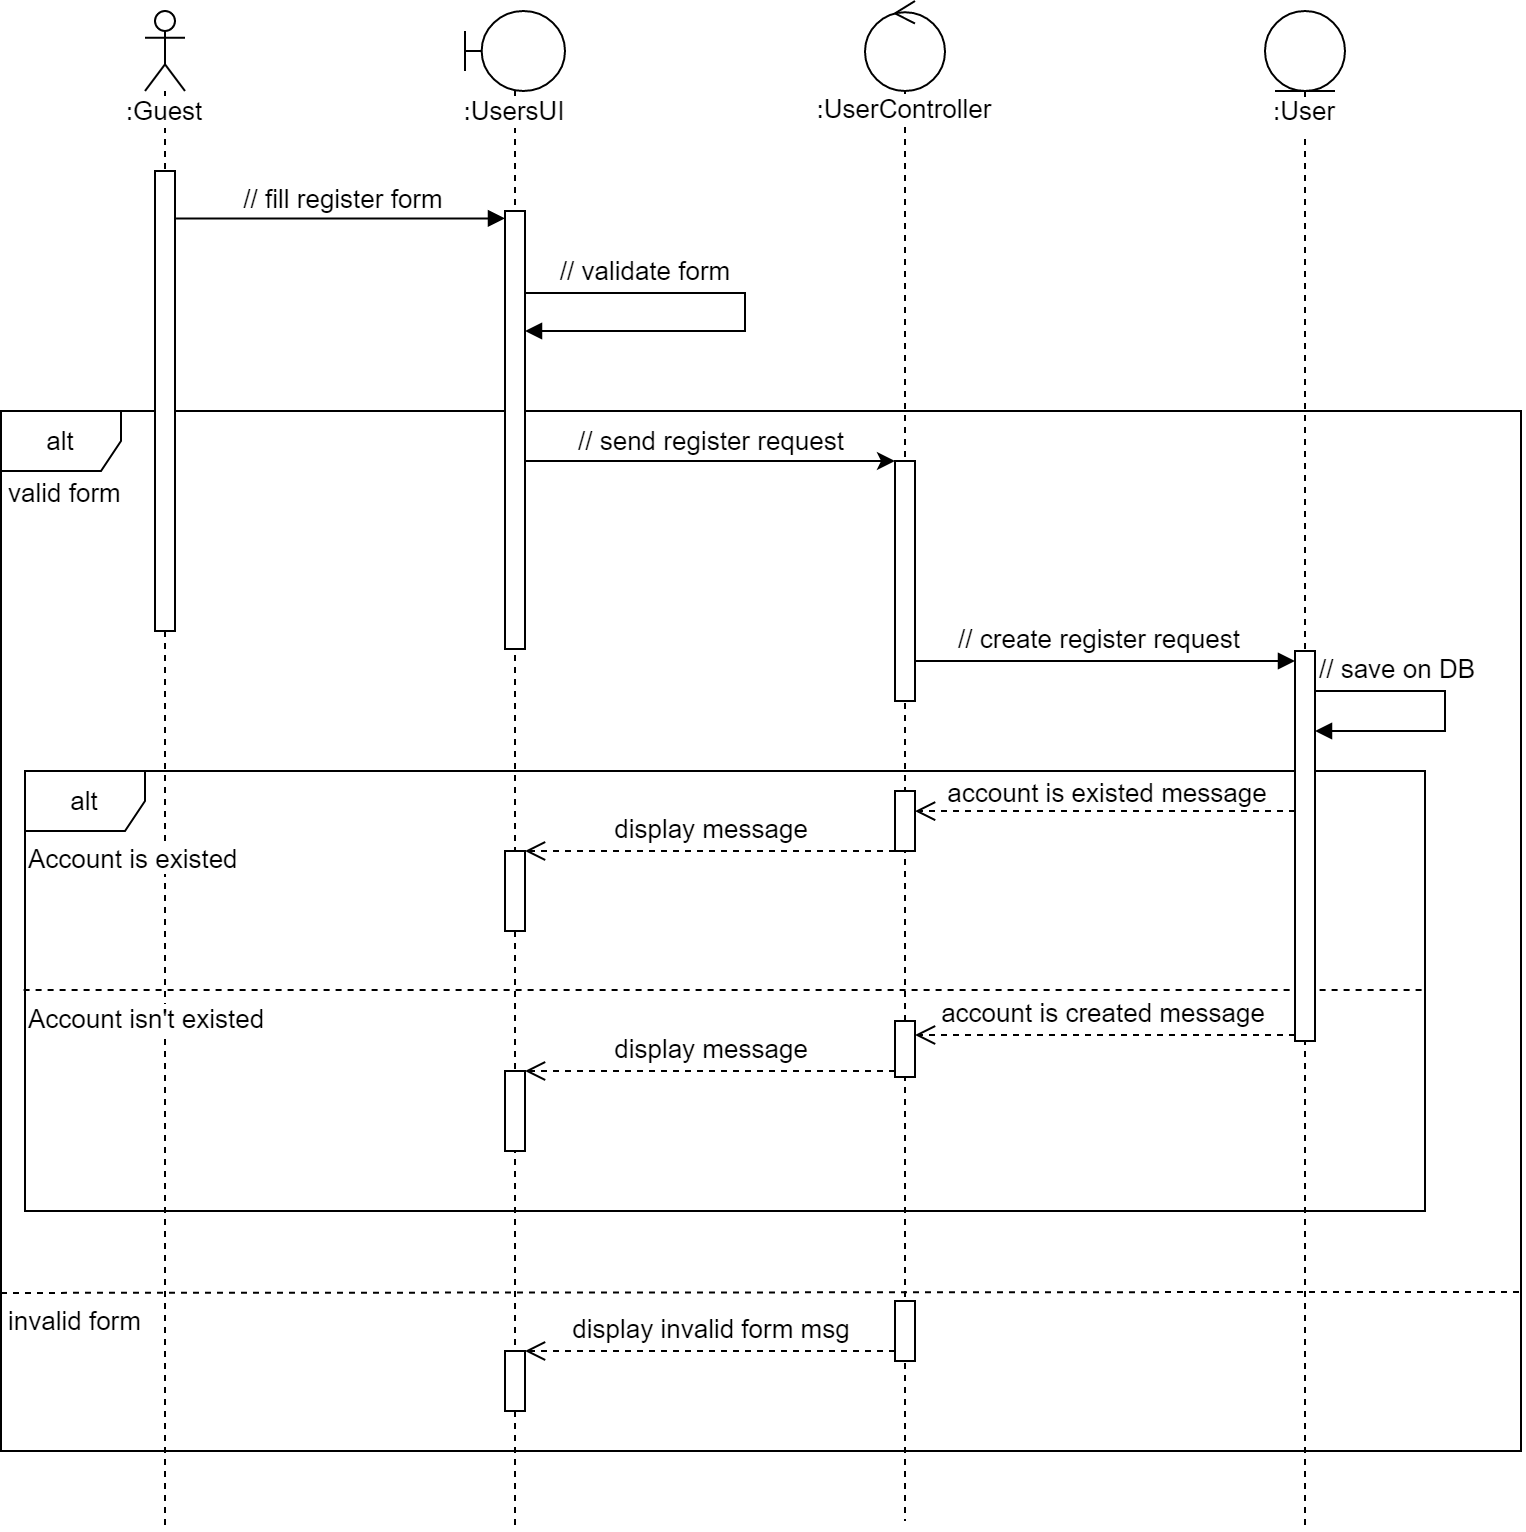
\includegraphics[width=\linewidth]{./img/uc1.png}
    \caption{\label{tab:seq-uc1}Biểu đồ tuần tự - Ca sử dụng Đăng ký}
\end{figure}
Hình \ref{tab:seq-uc1} mô tả quá trình đăng ký tài khoản như sau:
\begin{itemize}
    \item Khách truy cập hệ thống điền biểu mẫu đăng ký, nếu biểu mẫu không hợp lệ sẽ thông báo cho khách biết để sửa, nếu hợp lệ sẽ gửi biểu mẫu lên máy chủ.
    \item Máy chủ nhận được biểu mẫu sẽ kiểm tra trong cơ sở dữ liệu, nếu thông tin đăng ký hợp lệ sẽ lưu vào cơ sở dữ liệu và thông báo cho người dùng đăng ký tài khoản thành công, nếu thông tin đăng ký không hợp lệ sẽ trả ra cho khách biết lý do đăng ký tài khoản thất bại.
\end{itemize}

\subsection{Đăng nhập}
\begin{figure}[H]
	\centering
	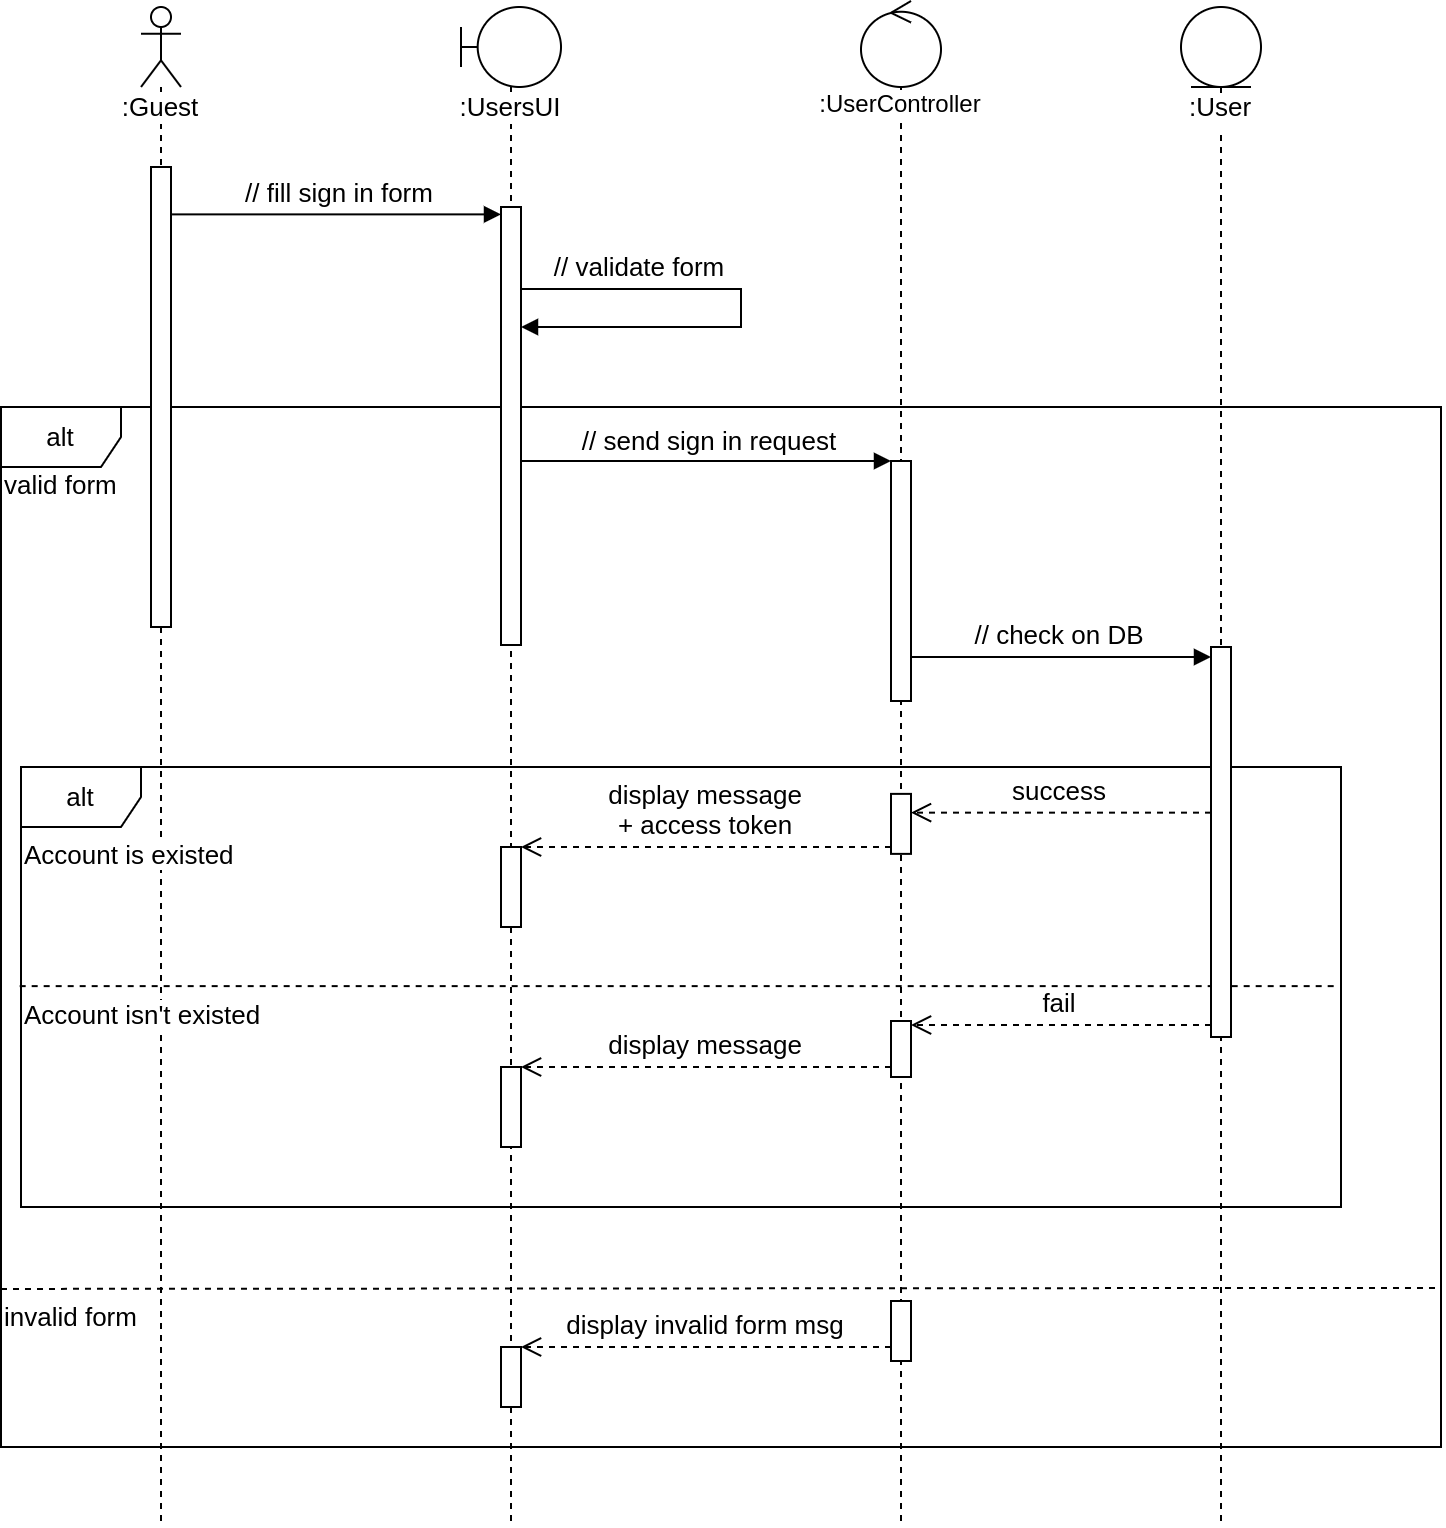
\includegraphics[width=\linewidth]{./img/uc2.png}
	\caption{\label{tab:seq-uc2}Biểu đồ tuần tự - Ca sử dụng Đăng nhập}
\end{figure}
Hình \ref{tab:seq-uc2} mô tả quá trình đăng nhập như sau:
\begin{itemize}
    \item Khách truy cập hệ thống điền biểu mẫu đăng nhập, nếu biểu mẫu không hợp lệ sẽ thông báo cho khách biết để sửa, nếu hợp lệ sẽ gửi biểu mẫu lên máy chủ.
    \item Máy chủ nhận được biểu mẫu sẽ kiểm tra trong cơ sở dữ liệu, nếu thông tin đăng nhập hợp lệ sẽ trả về thông báo cho khách biết đăng nhập thành công, nếu thông tin đăng nhập không hợp lệ sẽ trả ra cho khách biết lý do đăng nhập thất bại.
\end{itemize}

\subsection{Quên mật khẩu}
\begin{figure}[H]
	\centering
	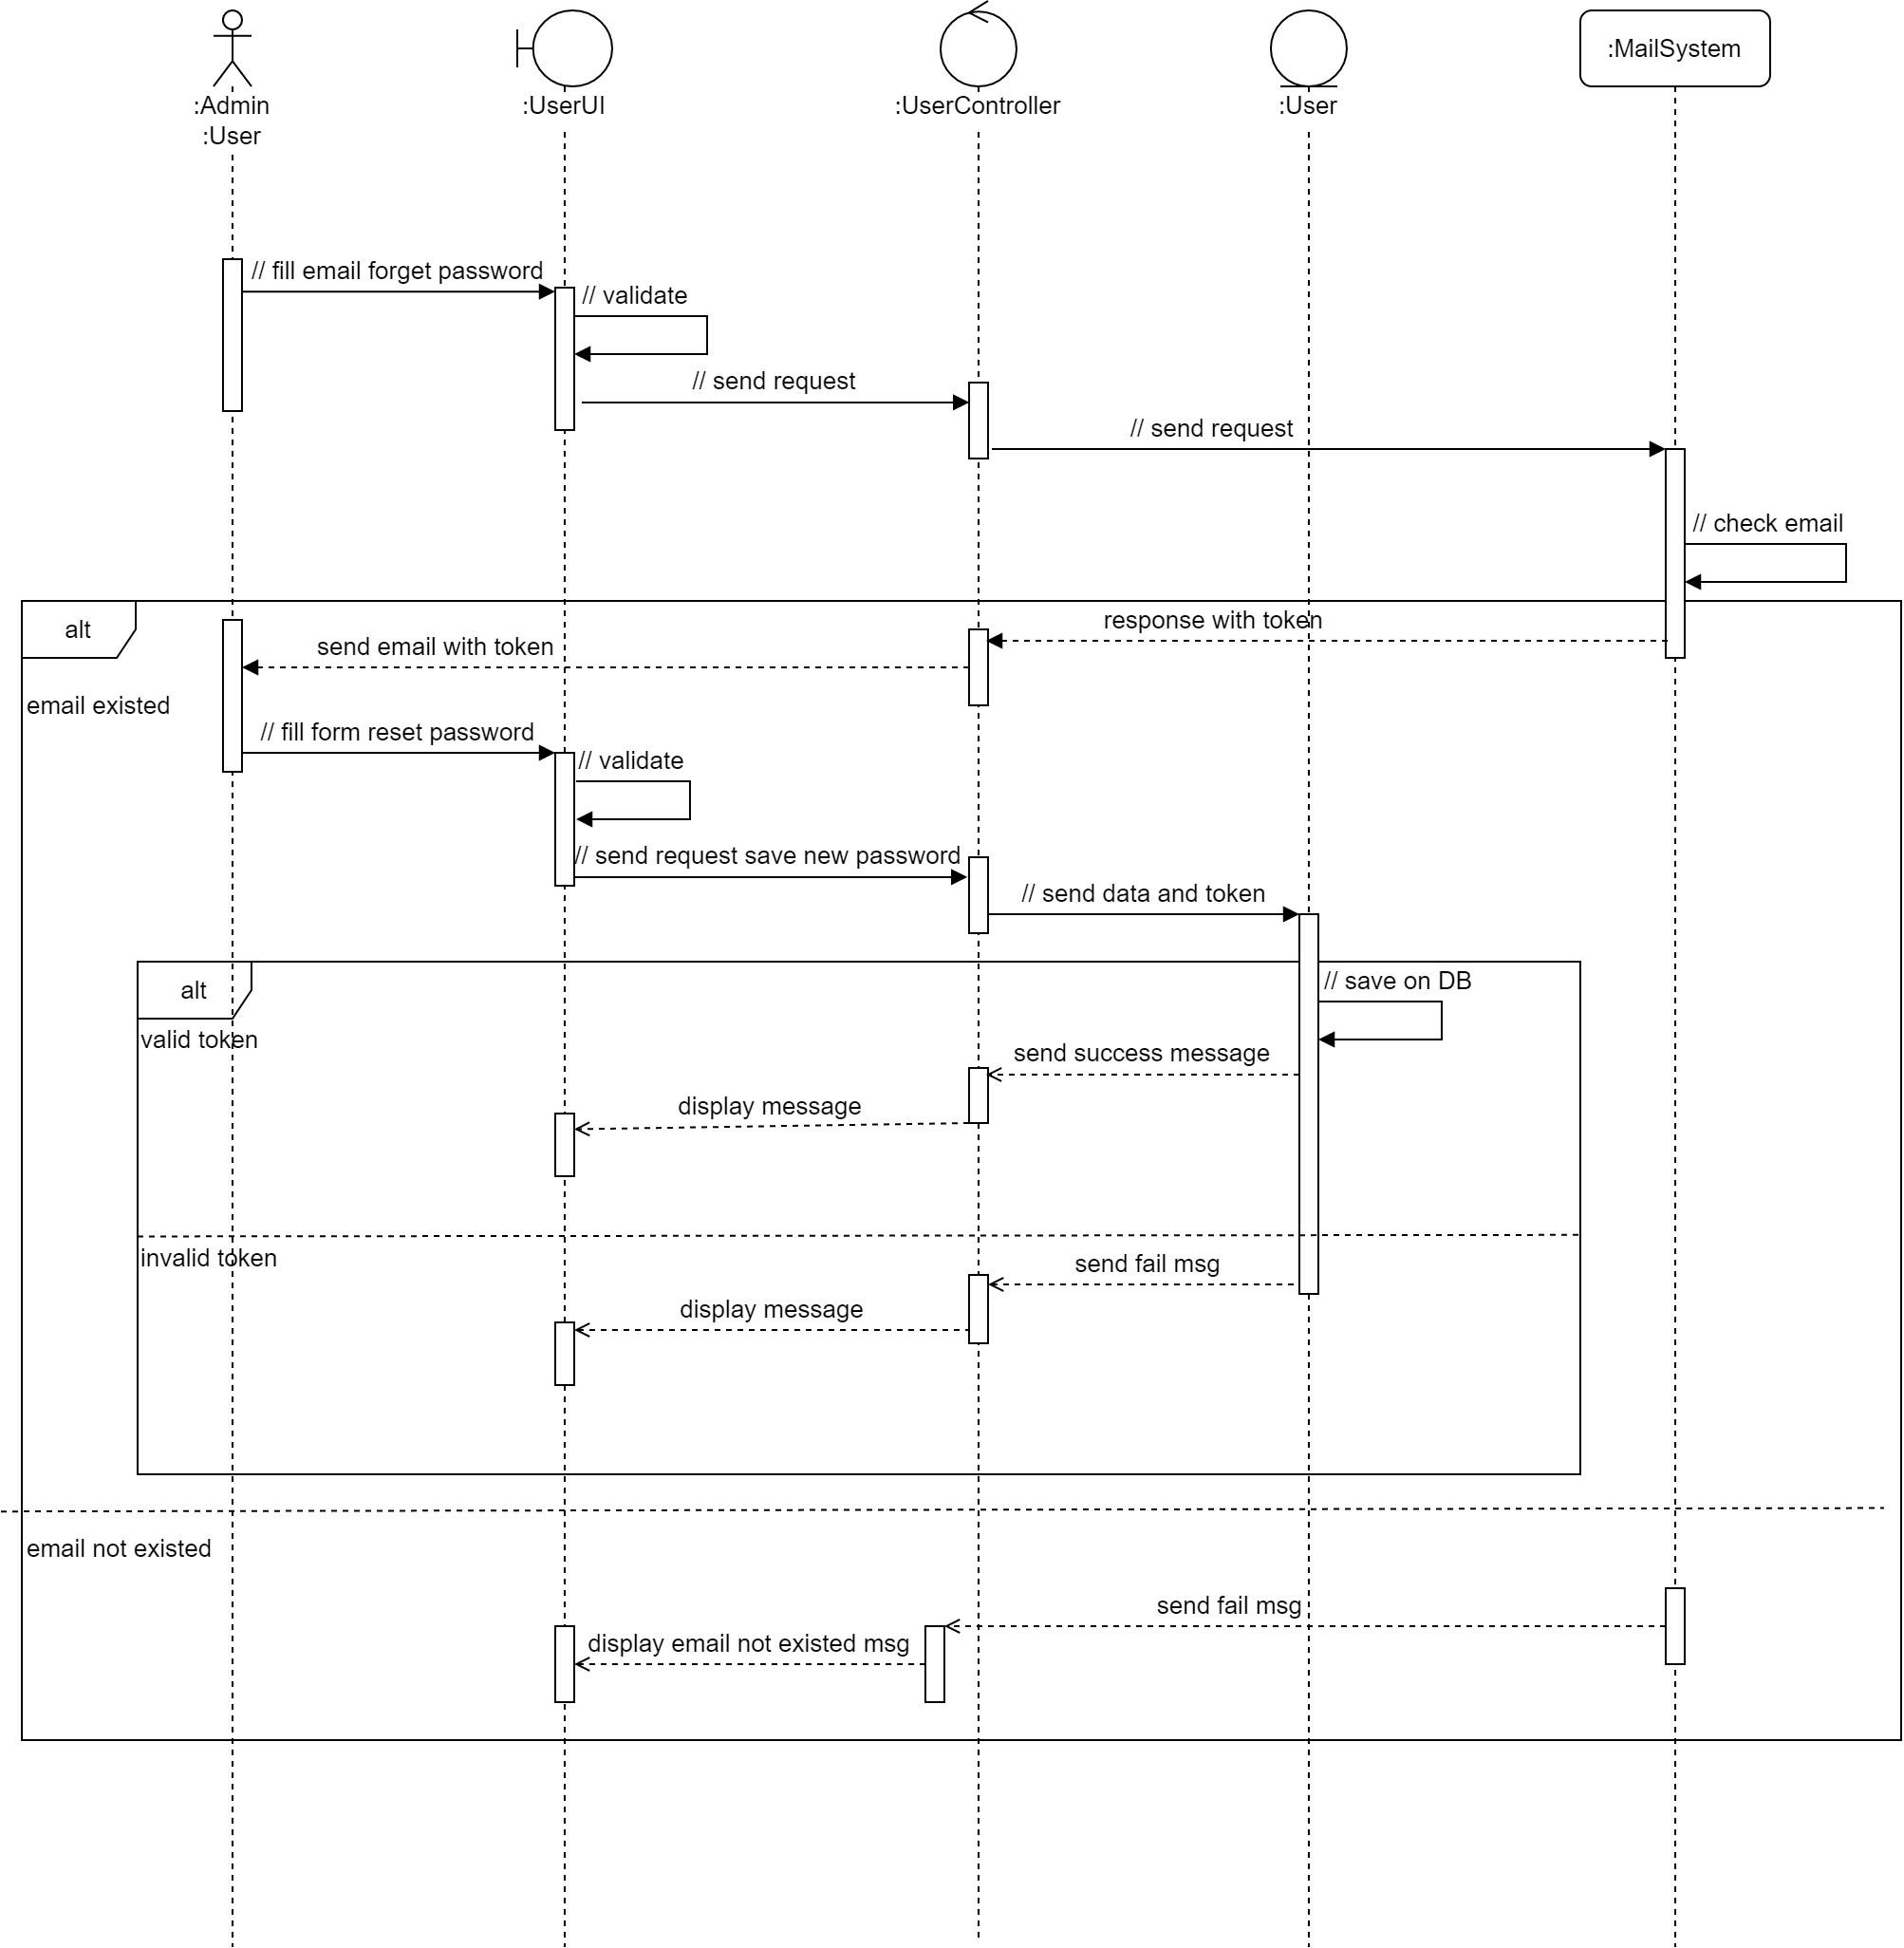
\includegraphics[width=\linewidth]{./img/uc3.png}
	\caption{\label{tab:seq-uc3}Biểu đồ tuần tự - Ca sử dụng Quên mật khẩu}
\end{figure}
Hình \ref{tab:seq-uc3} mô tả quá trình quên mật khẩu như sau:
\begin{itemize}
    \item Khách truy cập hệ thống chọn quên mật khẩu sẽ xuất hiện biểu mẫu, khách nhập thông tin theo biểu mẫu, nếu biểu mẫu không hợp lệ sẽ thông báo cho khách biết để sửa, nếu hợp lệ sẽ gửi biểu mẫu lên máy chủ.
    \item Máy chủ nhận được yêu cầu chứa biểu mẫu sẽ kiểm tra trong cơ sở dữ liệu, nếu thông tin biểu mẫu hợp lệ sẽ gửi liên kết đổi mật khẩu cho người dùng về hộp thư đã nhập và thông báo cho người dùng biết điều này, nếu thông tin biểu mẫu không hợp lệ sẽ trả ra cho khách biết lý do quên mật khẩu thất bại.
    \item Khách kiểm tra hộp thư, nhấp vào liên kết được gửi về hộp thư sẽ được điều hướng đến trang web có chứa biểu mẫu nhập mật khẩu mới.
    \item Khách điền thông tin theo biểu mẫu yêu cầu, nếu biểu mẫu không hợp lệ sẽ thông báo cho khách biết để sửa, nếu hợp lệ sẽ gửi biểu mẫu lên máy chủ.
    \item Máy chủ nhận được yêu cầu chứa mật khẩu mới, kiểm tra nếu yêu cầu hợp lệ sẽ lưu lại mật khẩu mới vào cơ sở dữ liệu và thông báo cho người dùng biết đổi mật khẩu thành công, nếu yêu cầu không hợp lệ sẽ thông báo cho người dùng biết lý do đổi mật khẩu thất bại.
\end{itemize}

Trong ca sử dụng Quên mật khẩu hệ thống có sử dụng \acrshort{smtp} của Gmail để gửi thư điện tử kèm đường dẫn giúp người dùng đổi mật khẩu. Khi người dùng gửi yêu cầu quên mật khẩu kèm email đã đăng ký, hệ thống sẽ thông qua \acrshort{smtp} gửi lại đường dẫn có chứa token đến trang đổi mật khẩu cho người dùng. Token có hạn sử dụng trong vòng 24 giờ kể từ khi hệ thống gửi thư điện tử. Nếu token còn hợp lệ thì khi cập nhật mới khẩu mới sẽ thành công. Nếu không thì mật khẩu vẫn giữ nguyên, không được thay đổi. Người dùng cần phải gửi yêu cầu quên mật khẩu mới nếu muốn thay đổi mật khẩu.

\subsection{Sửa thông tin tài khoản}
\begin{figure}[H]
	\centering
	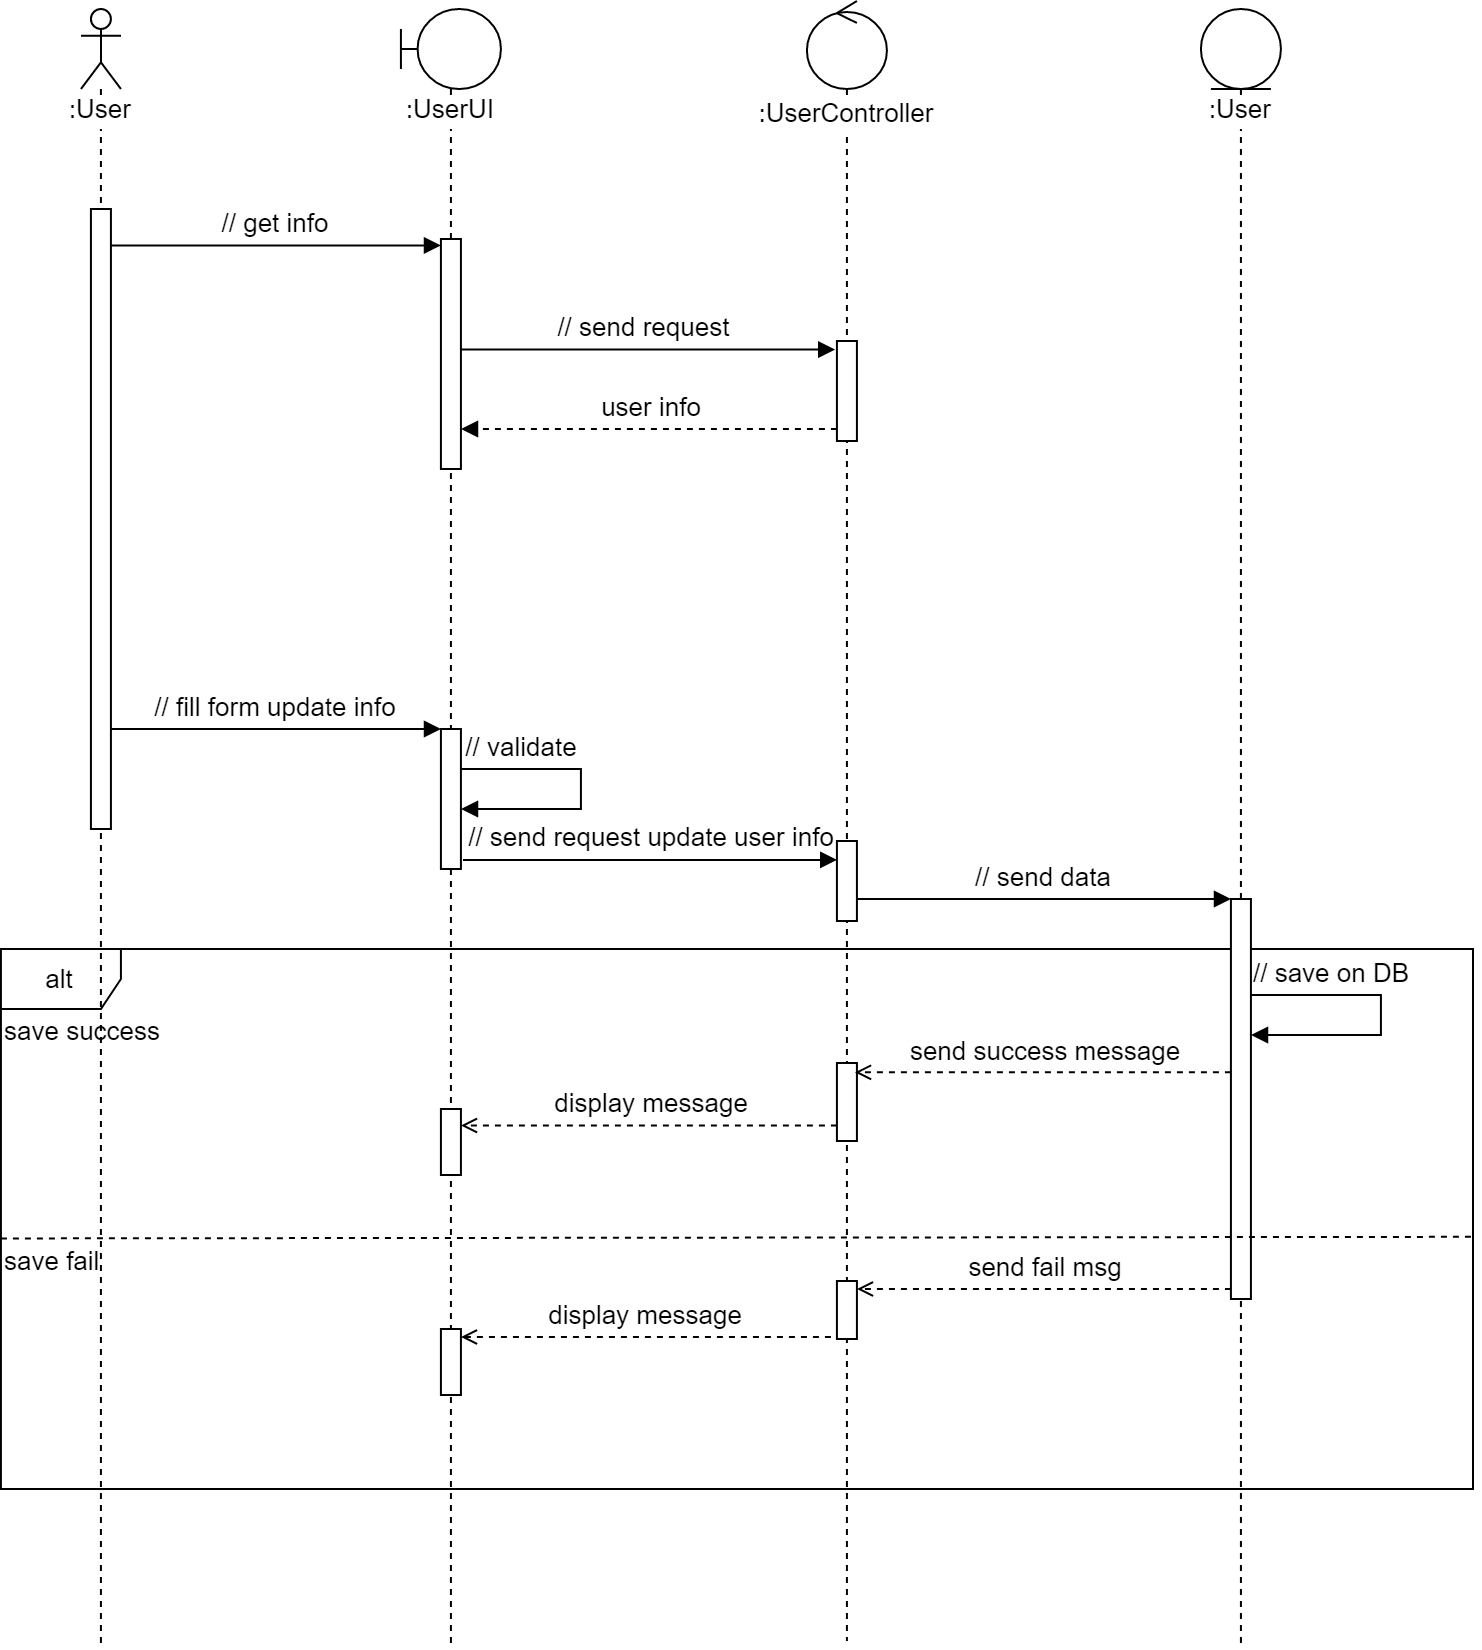
\includegraphics[width=\linewidth]{./img/uc4.png}
	\caption{\label{tab:seq-uc4}Biểu đồ tuần tự - Ca sử dụng Sửa thông tin tài khoản}
\end{figure}
Hình \ref{tab:seq-uc4} mô tả quá trình sửa thông tin tài khoản như sau:
\begin{itemize}
    \item Người dùng truy cập vào trang thông tin tài khoản sẽ gửi một yêu cầu lên máy chủ để lấy thông tin. Máy chủ kiểm tra yêu cầu, nếu hợp lệ sẽ trả về thông tin tài khoản cho người dùng.
    \item Người dùng chọn sửa thông tin, nhập thông tin cần sửa vào biểu mẫu và chọn cập nhật, nếu biểu mẫu không hợp lệ sẽ thông báo cho người dùng biết để sửa, nếu hợp lệ sẽ gửi biểu mẫu lên máy chủ.
    \item Máy chủ nhận được yêu cầu sửa thông tin, kiểm tra yêu cầu và biểu mẫu, nếu hợp lệ sẽ lưu lại thông tin mới vào cơ sở dữ liệu và thông báo cho người dùng biết sửa thông tin thành công, nếu không hợp lệ sẽ thông báo cho người dùng biết lý do sửa thất bại.
\end{itemize}


\subsection{Đăng xuất}
\begin{figure}[H]
	\centering
	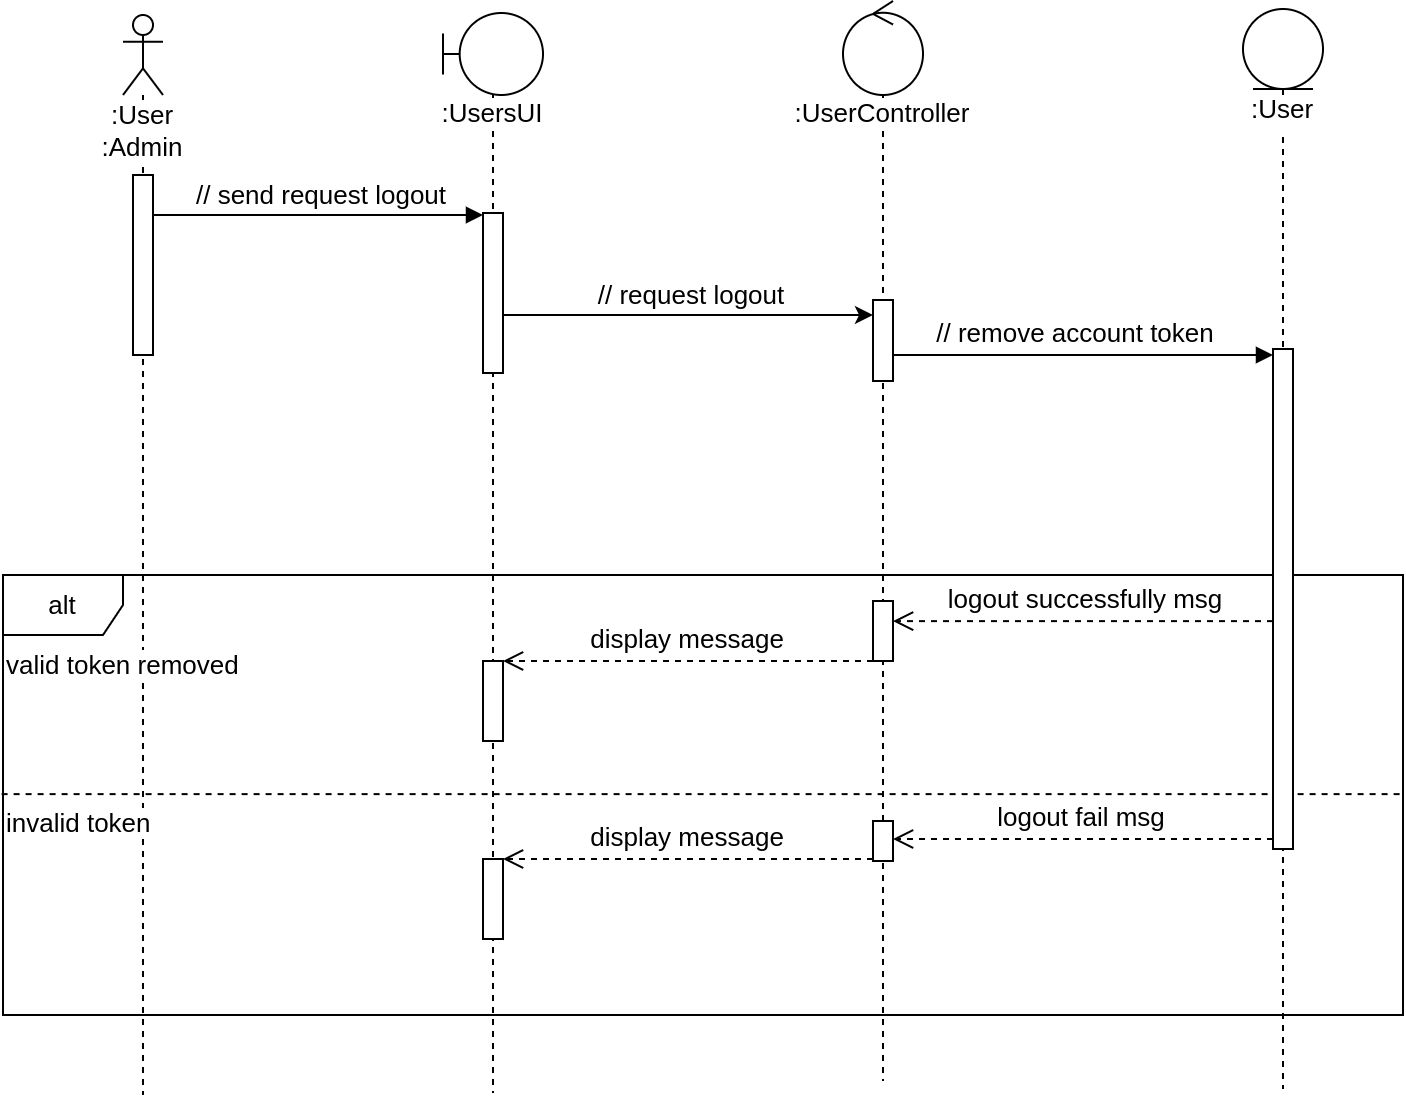
\includegraphics[width=\linewidth]{./img/uc5.png}
	\caption{\label{tab:seq-uc5}Biểu đồ tuần tự - Ca sử dụng Đăng xuất}
\end{figure}
Hình \ref{tab:seq-uc5} mô tả quá trình đăng xuất như sau:
\begin{itemize}
    \item Người dùng nhấn đăng xuất nằm trong phần tùy chọn của dưới tài khoản trên thanh điều hướng, phần mềm sẽ gửi yêu cầu lên máy chủ.
    \item Máy chủ kiểm tra yêu cầu, nếu hợp lệ sẽ thông báo cho người dùng biết đăng xuất thành công, nếu không sẽ thông báo cho người dùng biết lý do đăng xuất thất bại.
\end{itemize}

\subsection{Các ca sử dụng xem và tìm kiếm dữ liệu}
\begin{figure}[H]
	\centering
	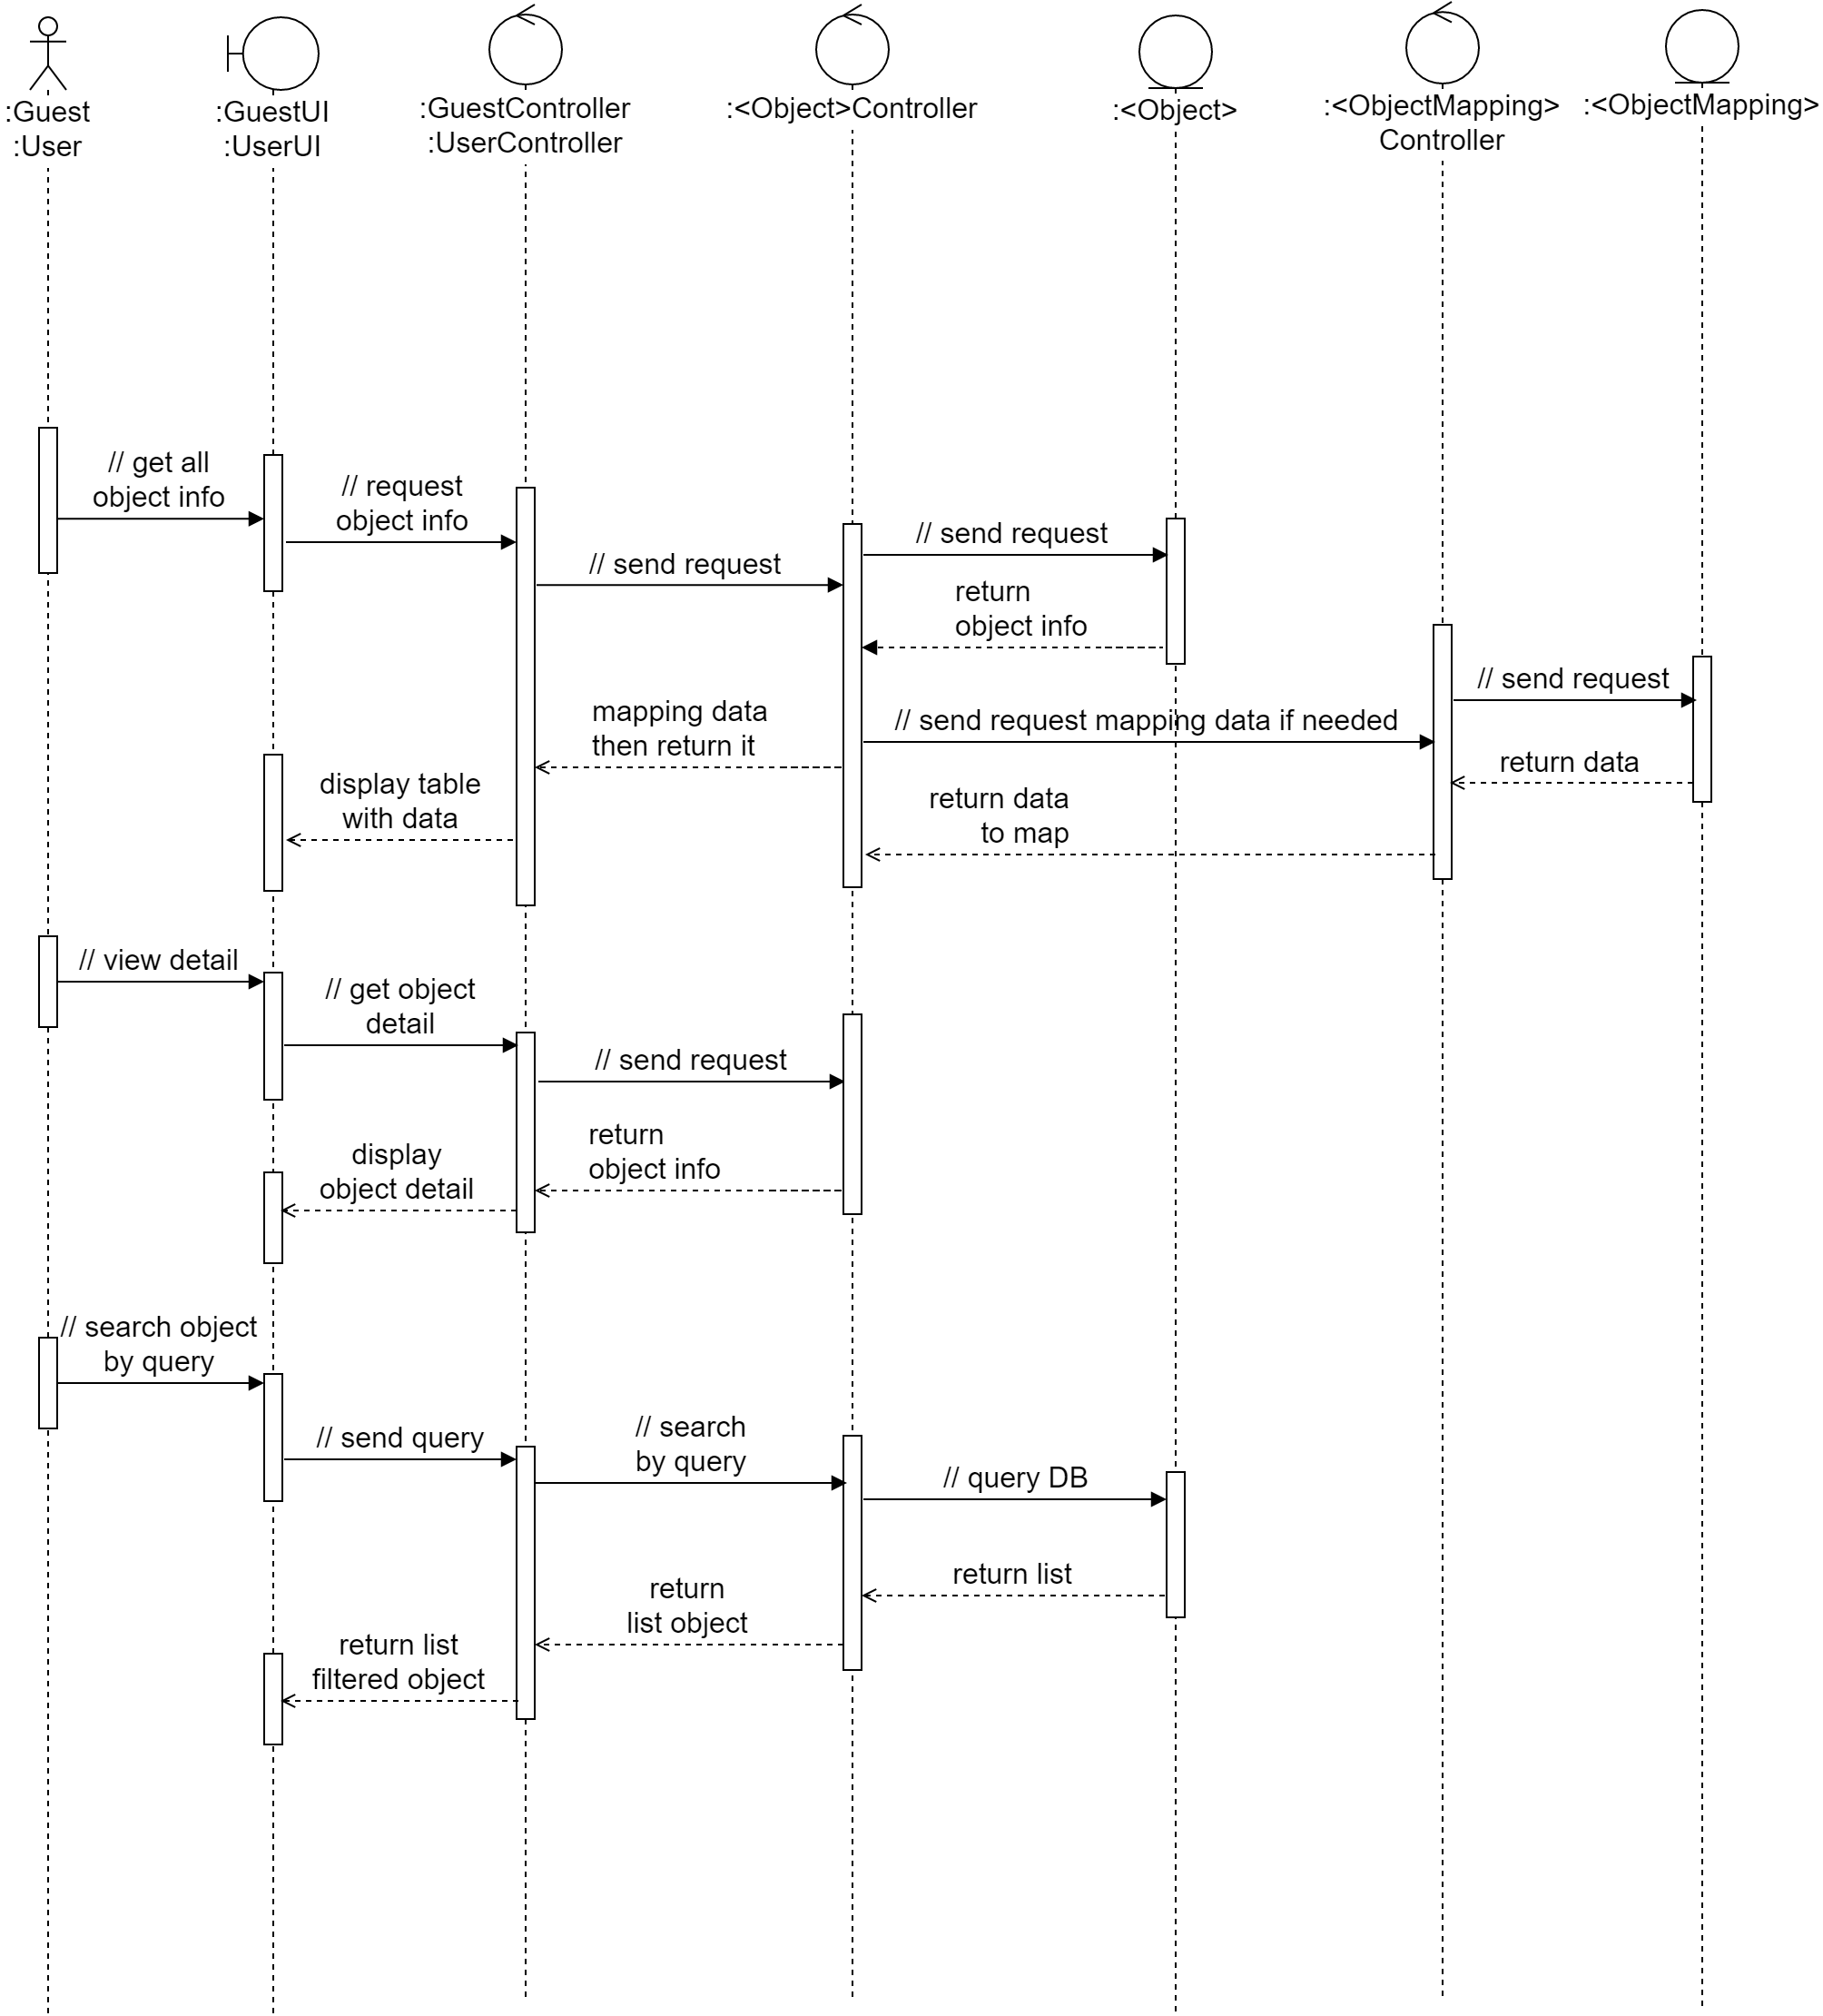
\includegraphics[width=\linewidth]{./img/uc6-11.png}
	\caption{\label{tab:seq-uc6}Biểu đồ tuần tự - Các ca sử dụng xem và tìm kiếm dữ liệu}
\end{figure}
Hình \ref{tab:seq-uc6} mô tả quá trình xem và tìm kiếm dữ liệu như sau:
\begin{itemize}
    \item Người dùng gửi yêu cầu lấy thông tin về tất cả đối tượng, yêu cầu này có thể bao gồm từ khóa tìm kiếm hay các thuộc tính của bộ lọc.
    \item Máy chủ kiểm tra yêu cầu, nếu hợp lệ sẽ thực hiện truy vấn trong cơ sở dữ liệu để lấy thông tin về đối tượng, tùy vào yêu cầu gửi lên nếu có từ khóa hay bộ lọc sẽ thực hiện thêm truy vấn để tìm kiếm và lọc dữ liệu theo yêu cầu rồi trả về thông tin các đối tượng phù hợp với yêu cầu cho người dùng.
    \item Người dùng gửi yêu cầu xem chi tiết một đối tượng, máy chủ nhận được yêu cầu, hợp lệ sẽ trả về thông tin chi tiết của đối tượng đó cho người dùng.
\end{itemize}
Các ca sử dụng xem và tìm kiếm dữ liệu có thể khá tương đồng nhau trong luồng hoạt động. Có một số bảng dữ liệu không cần liên kết với các bảng dữ liệu khác để hiển thị đầy đủ thông tin, chúng có thể đứng độc lập, như là: dữ liệu về sắn, bệnh về sắn,... Tuy nhiên cũng có những bảng dữ liệu cần liên kết với một hay nhiều bảng dữ liệu khác để hiển thị được đầy đủ, chẳng hạn: dữ liệu về bản đồ sắn, dữ liệu về thương mại sắn,...

Cụ thể bảng dữ liệu về bản đồ sắn biểu thị thông tin về dịch bệnh sắn ở Tây Ninh trên bản đồ cần liên kết với bảng dữ liệu sắn thông qua nhãn sắn, bệnh về sắn thông qua nhãn bệnh cũng như tọa độ địa lý các khu vực ở Tây Ninh thông qua mã khu vực, từ đó hiển thị được đúng và đủ dữ liệu. Để phục vụ cho việc vẽ bản đồ, hệ thống sử dụng Leaflet.

\subsection{Chẩn đoán bệnh trên cây sắn}
\begin{figure}[H]
	\centering
	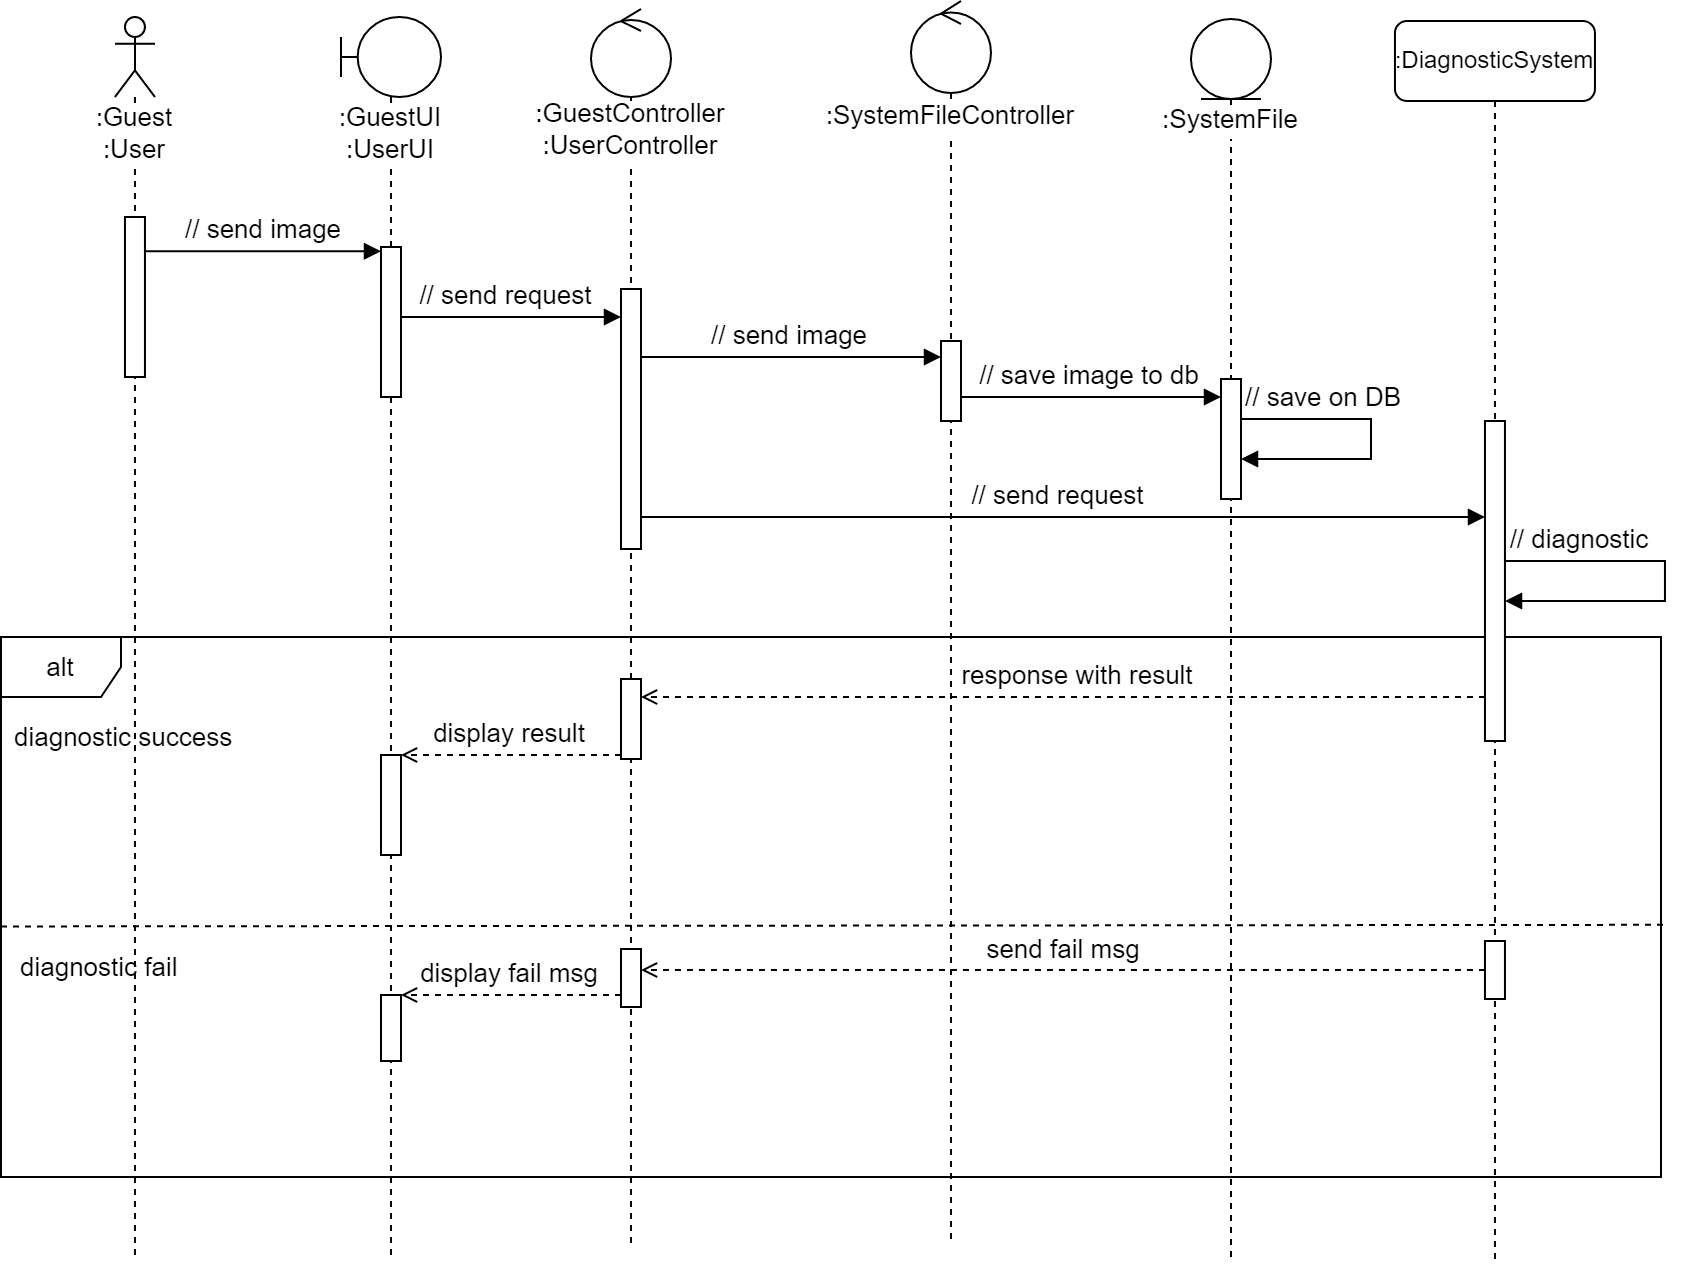
\includegraphics[width=\linewidth]{./img/uc12.png}
	\caption{\label{tab:seq-uc7}Biểu đồ tuần tự - Ca sử dụng Chẩn đoán bệnh trên cây sắn}
\end{figure}
Hình \ref{tab:seq-uc7} mô tả quá trình chẩn đoán bệnh trên cây sắn như sau:
\begin{itemize}
    \item Người dùng tải tệp ảnh lên, chọn đăng ảnh, nếu tệp ảnh hợp lệ sẽ gửi yêu cầu lên máy chủ .
    \item Máy chủ kiểm tra yêu cầu, hợp lệ sẽ lưu ảnh vào trong cơ sở dữ liệu và gửi một yêu cầu sang hệ thống chẩn đoán.
    \item Hệ thống chẩn đoán tiếp nhận và xử lý yêu cầu, nếu xử lý thành công sẽ trả về cho người dùng thông tin các bệnh chuẩn đoán được, nếu thất bại sẽ thông báo cho người dùng thông báo chẩn đoán thất bại.
\end{itemize}

\subsection{Tạo nhận xét}
\begin{figure}[H]
	\centering
	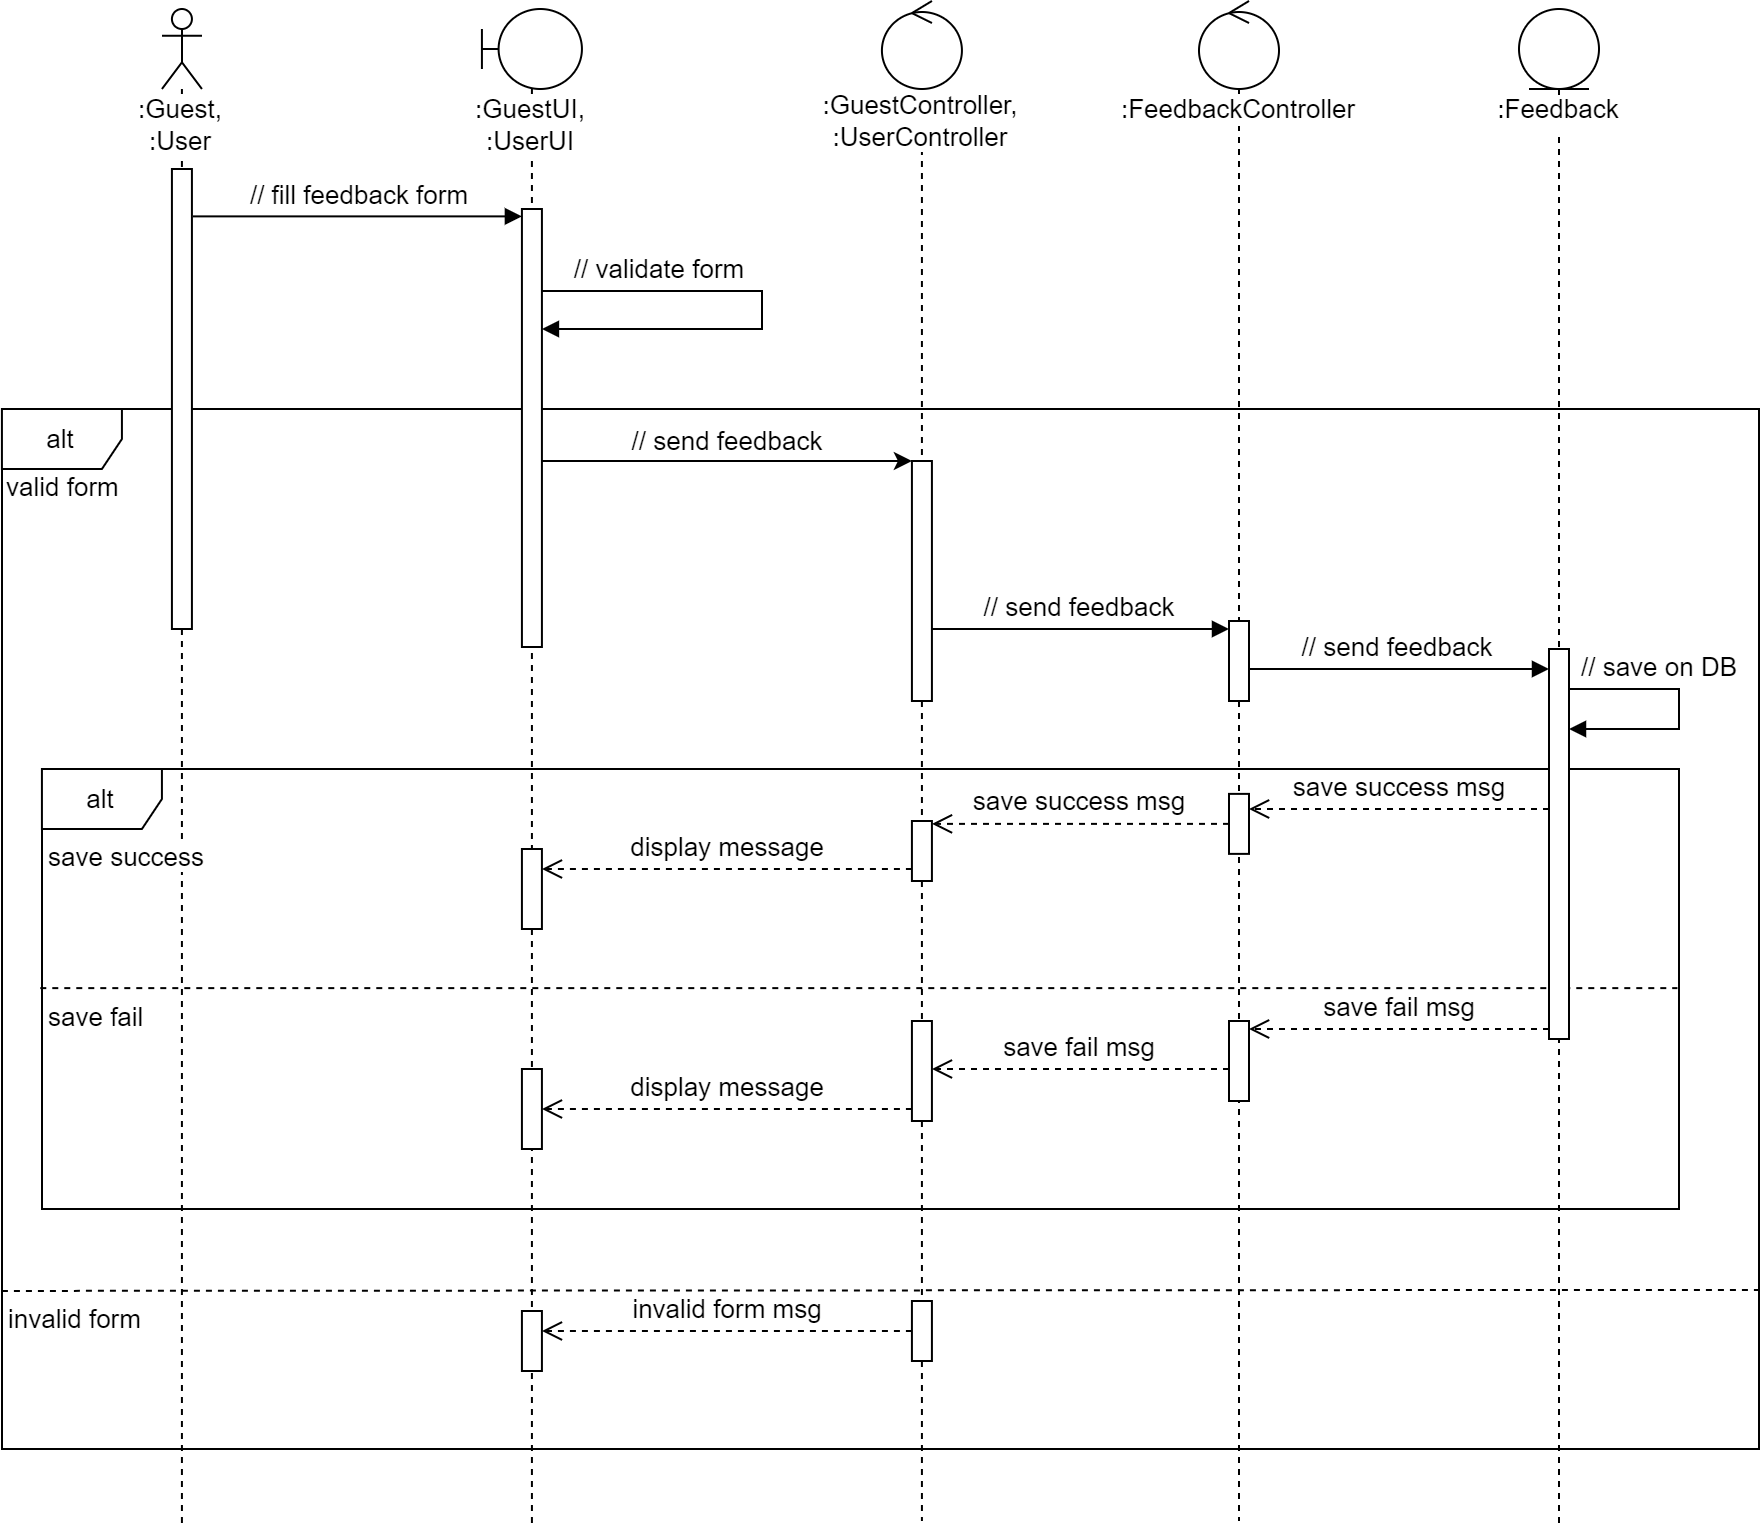
\includegraphics[width=\linewidth]{./img/uc13.png}
	\caption{\label{tab:seq-uc8}Biểu đồ tuần tự - Ca sử dụng Tạo nhận xét}
\end{figure}
Hình \ref{tab:seq-uc8} mô tả quá trình tạo nhận xét như sau:
\begin{itemize}
    \item Người dùng điền thông tin vào biểu mẫu tạo nhận xét, nếu biểu mẫu không hợp lệ sẽ thông báo cho người dùng biết để sửa, nếu hợp lệ sẽ gửi biểu mẫu lên máy chủ.
    \item Máy chủ kiểm tra yêu cầu, hợp lệ sẽ lưu lại thông tin trong cơ sở dữ liệu và trả về thông báo tạo nhận xét thành công, nếu không hợp lệ sẽ trả về thông báo tạo nhận xét thất bại.
\end{itemize}

\subsection{Quản lý đề xuất trên sàn thương mại sắn}
\begin{figure}[H]
	\centering
	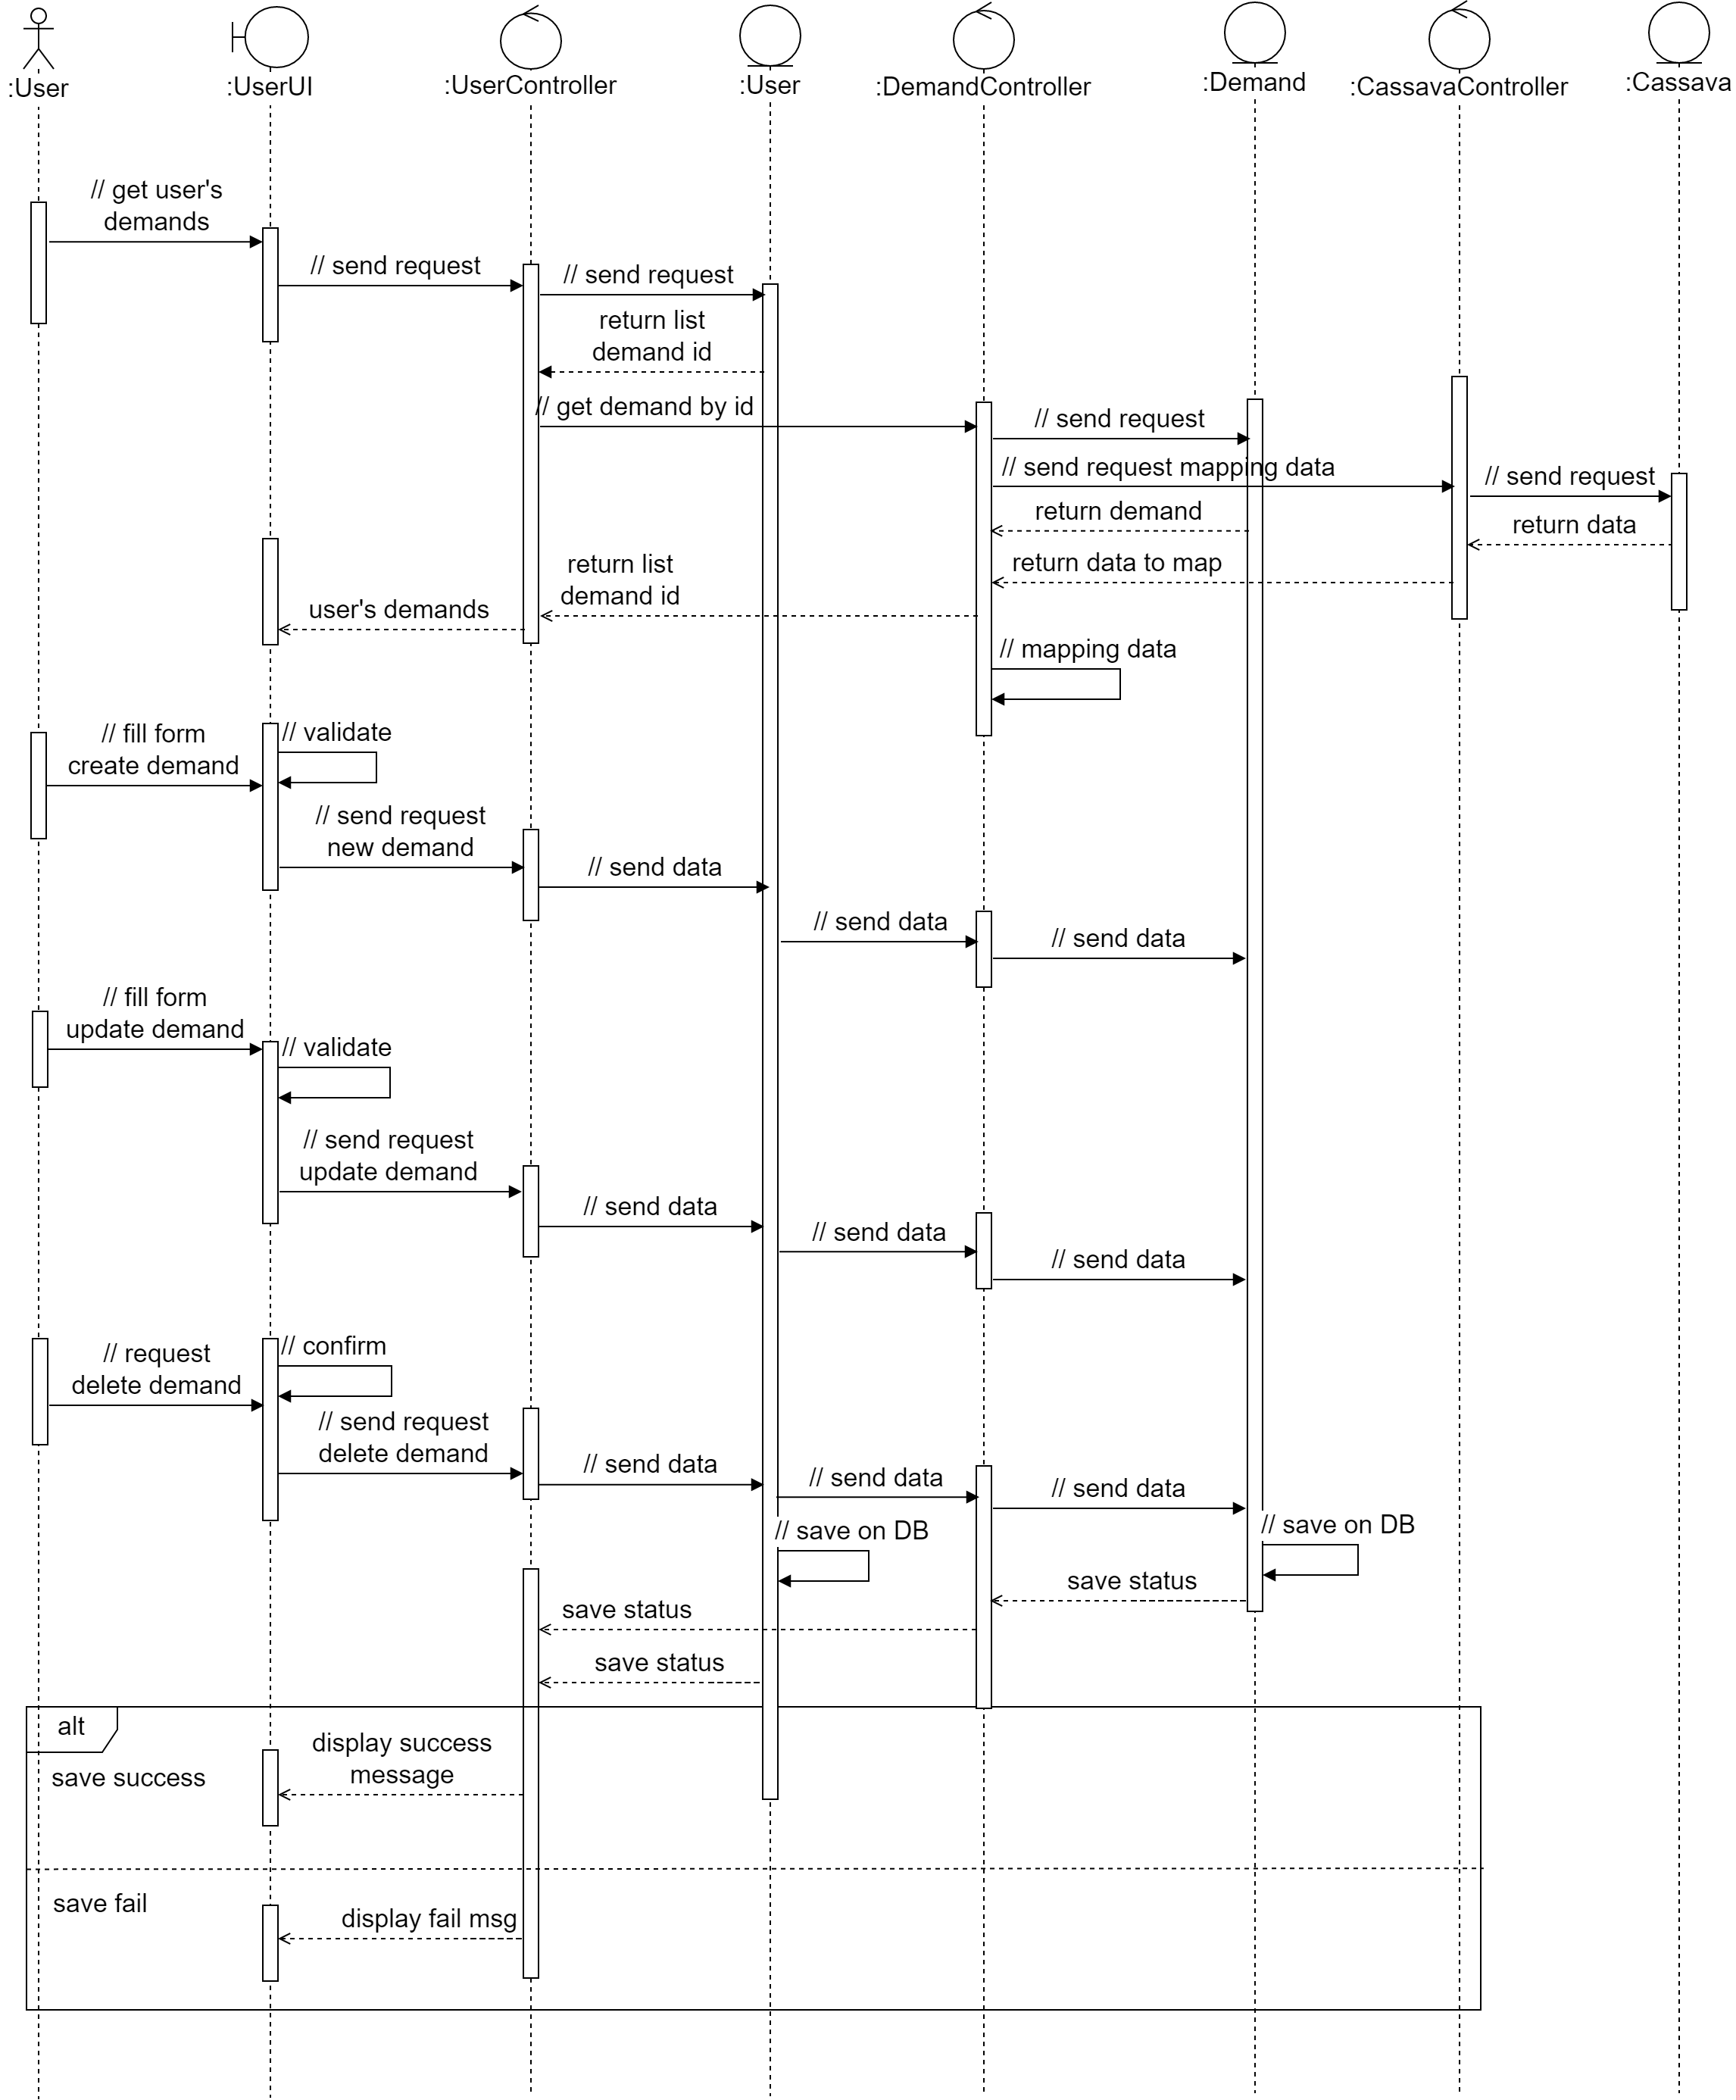
\includegraphics[width=\linewidth]{./img/uc14.png}
	\caption{\label{tab:seq-uc9}Biểu đồ tuần tự - Ca sử dụng Quản lý đề xuất thương mại sắn}
\end{figure}
Hình \ref{tab:seq-uc9} mô tả quá trình quản lý đề xuất trên sàn thương mại sắn như sau:
\begin{itemize}
    \item Người dùng gửi yêu cầu lấy danh sách đề xuất lên máy chủ, yêu cầu này có thể bao gồm từ khóa để tìm kiếm hoặc tùy chọn lọc.
    \item Máy chủ kiểm tra yêu cầu, nếu hợp lệ, sẽ tùy thuộc vào yêu cầu có thêm từ khóa tìm kiếm hay tùy chọn lọc hay không mà máy chủ thực hiện truy vấn phù hợp trong cơ sở dữ liệu để lấy danh sách đề xuất thỏa mãn yêu cầu để trả về cho người dùng.
    \item Người dùng chọn tạo hoặc cập nhật đề xuất, sẽ xuất hiện biểu mẫu cho người dùng nhập thông tin và ấn gửi, nếu thông tin được nhập hợp lệ sẽ gửi yêu cầu lên máy chủ, nếu không hợp lệ sẽ thông báo cho người dùng biết để sửa.
    \item Máy chủ tiếp nhận yêu cầu tạo hoặc cập nhật đề xuất, nếu yêu cầu hợp lệ sẽ lưu lại thông tin vào trong cơ sở dữ liệu và thông báo cho người dùng yêu cầu thành công, nếu không hợp lệ thông báo cho người dùng biết yêu cầu thất bại.
    \item Người dùng chọn xóa đề xuất và ấn xác nhận sẽ gửi yêu cầu xóa đề xuất lên máy chủ.
    \item Máy chủ nhận được yêu cầu xóa đề xuất, thực hiện yêu cầu, nếu thành công sẽ xóa đề xuất trong cơ sở dữ liệu và thông báo cho người dùng xóa đề xuất thành công, nếu xóa thất bại sẽ thông báo cho người dùng xóa đề xuất thất bại.
\end{itemize}

\subsection{Xem và tạo bài viết trên diễn đàn}

\begin{figure}[H]
	\centering
	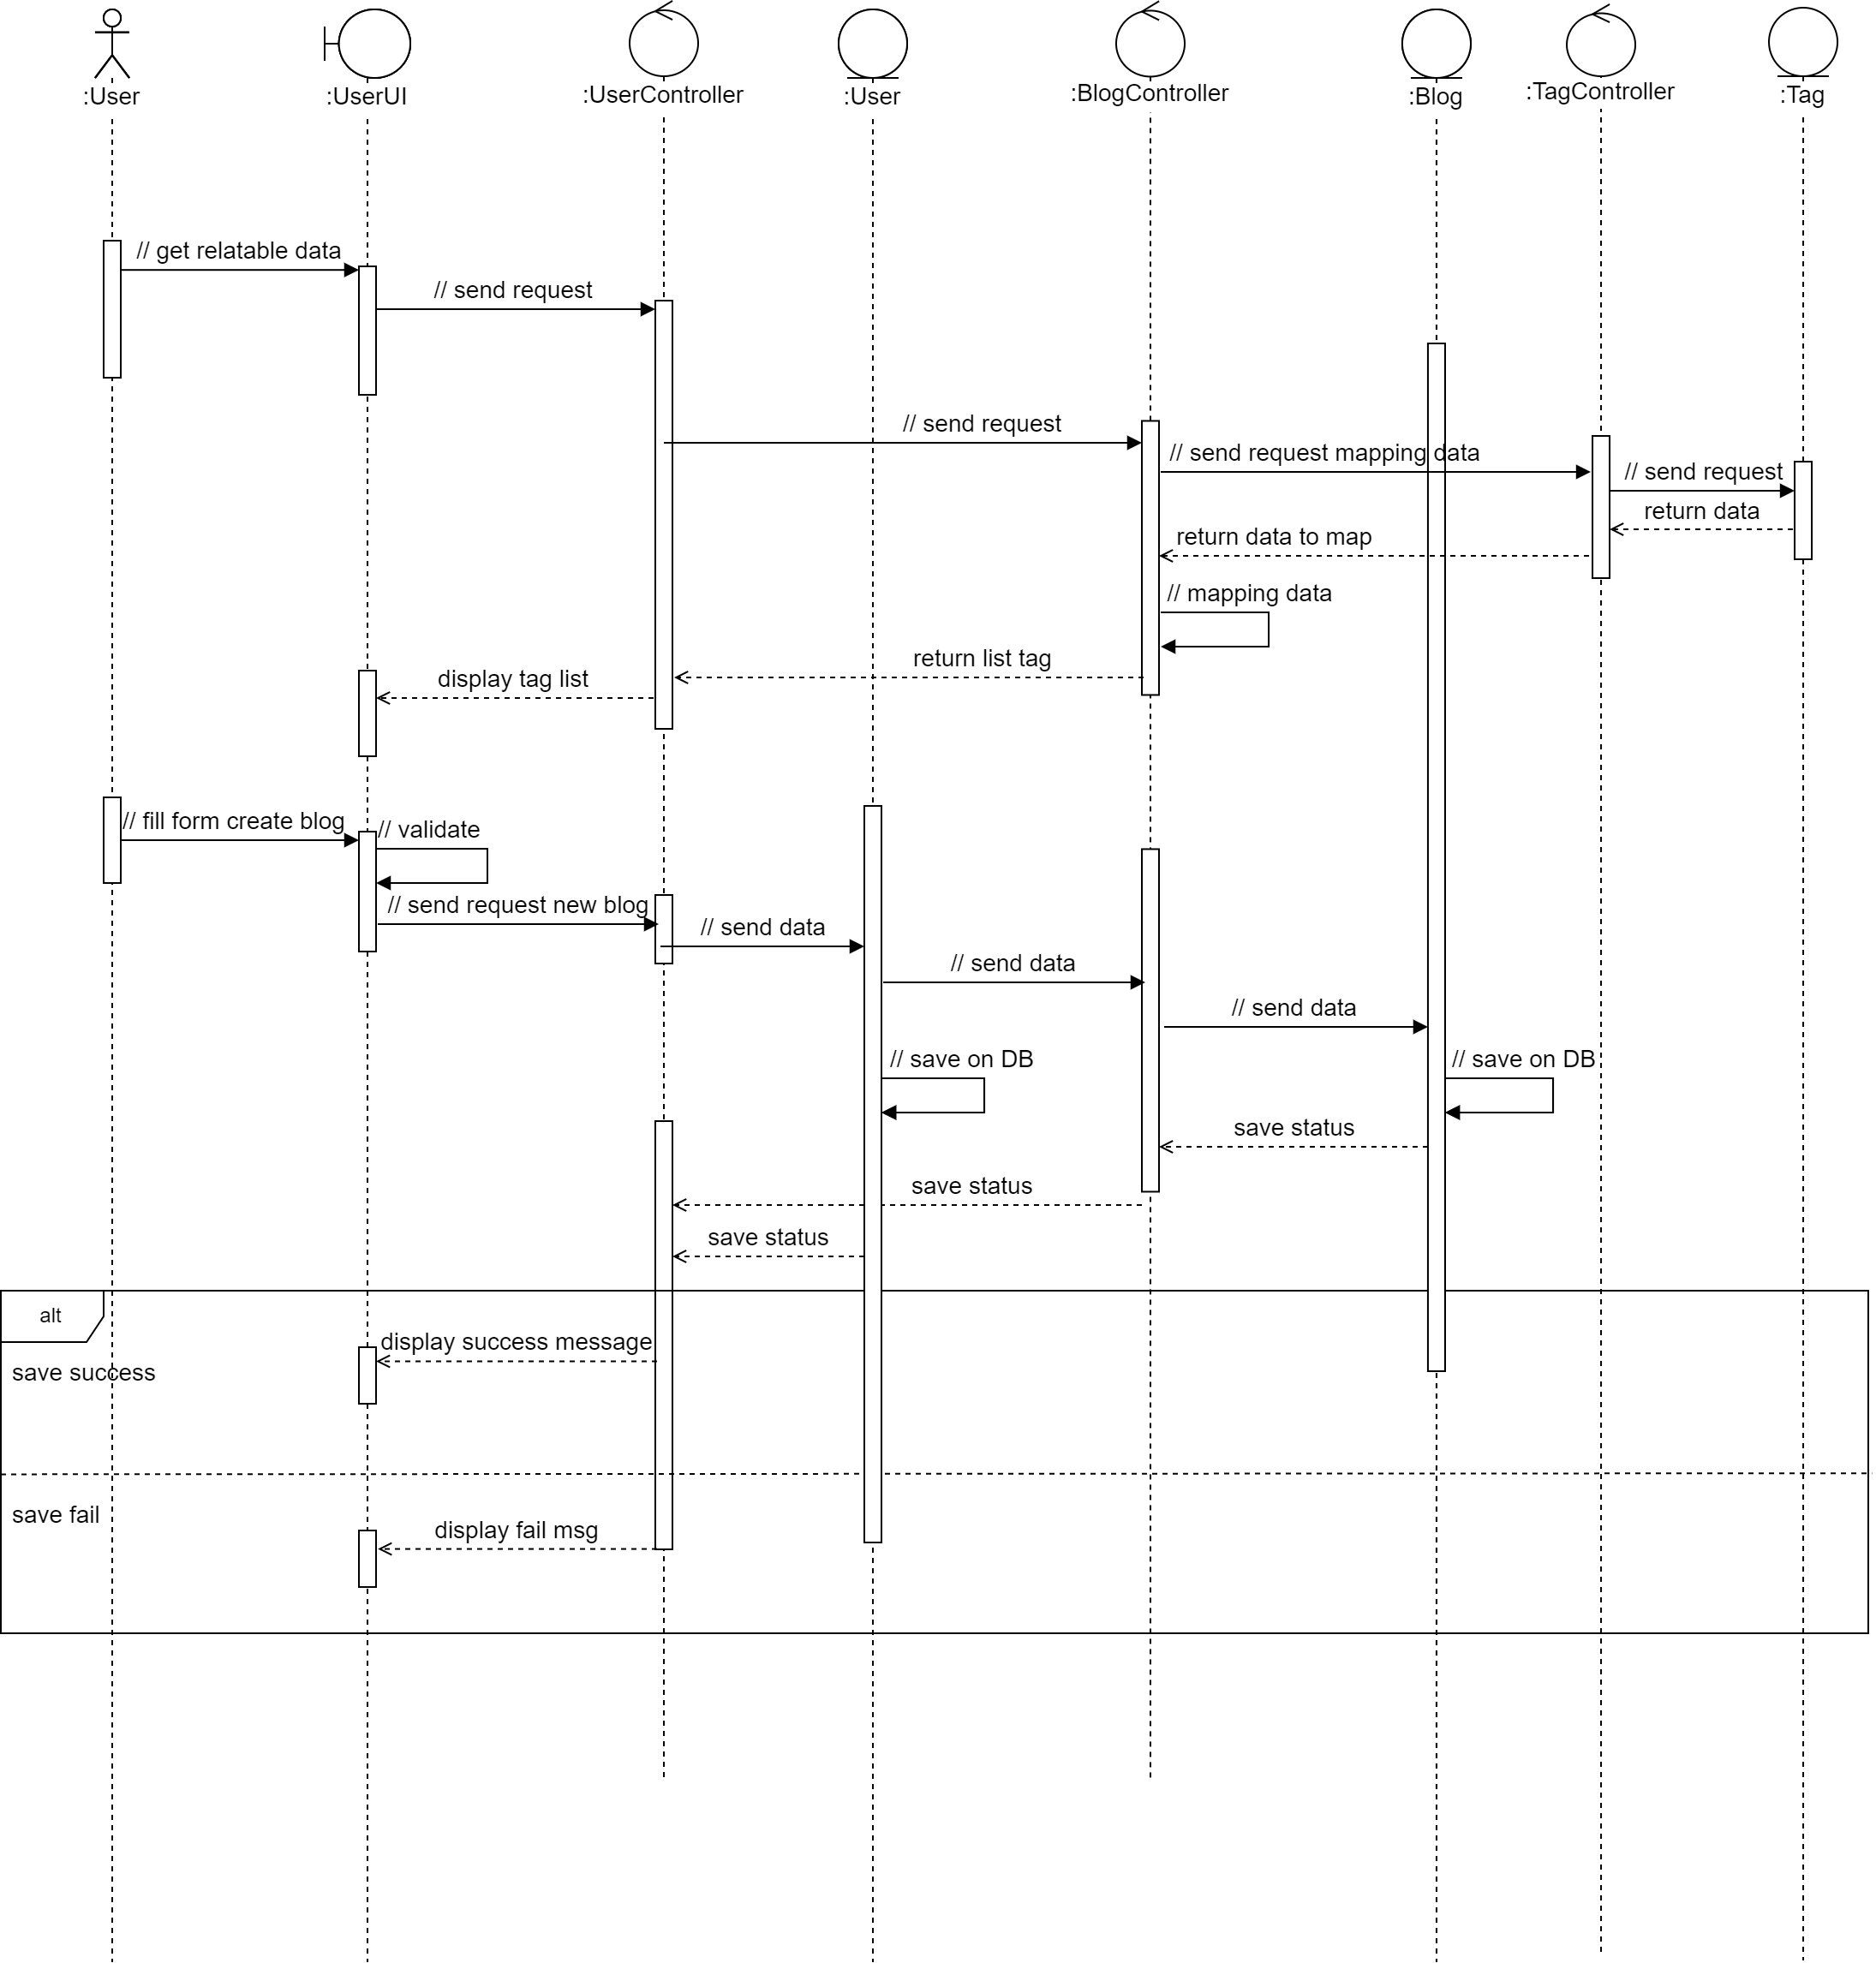
\includegraphics[width=\linewidth]{./img/uc15.png}
	\caption{\label{tab:seq-uc10}Biểu đồ tuần tự - Ca sử dụng Xem và tạo bài viết trên diễn đàn}
\end{figure}

Hình \ref{tab:seq-uc10} mô tả quá trình xem và tạo bài viết trên diễn đàn như sau:
\begin{itemize}
    \item Người dùng gửi yêu cầu lấy danh sách bài viết lên máy chủ, yêu cầu này có thể bao gồm từ khóa để tìm kiếm hoặc tùy chọn lọc.
    \item Máy chủ kiểm tra yêu cầu, nếu hợp lệ, sẽ tùy thuộc vào yêu cầu có thêm từ khóa tìm kiếm hay tùy chọn lọc hay không mà máy chủ thực hiện truy vấn phù hợp trong cơ sở dữ liệu để lấy danh sách bài viết thỏa mãn yêu cầu để trả về cho người dùng.
    \item Người dùng chọn tạo bài viết, sẽ xuất hiện biểu mẫu cho người dùng nhập thông tin và ấn gửi, nếu thông tin được nhập hợp lệ sẽ gửi yêu cầu lên máy chủ, nếu không hợp lệ sẽ thông báo cho người dùng biết để sửa.
    \item Máy chủ tiếp nhận yêu cầu tạo bài viết, nếu yêu cầu hợp lệ sẽ lưu lại thông tin vào trong cơ sở dữ liệu và thông báo cho người dùng yêu cầu thành công, nếu không hợp lệ thông báo cho người dùng biết yêu cầu thất bại.
\end{itemize}

\subsection{Các ca sử dụng quản lý của Quản trị viên}
\begin{figure}[H]
	\centering
	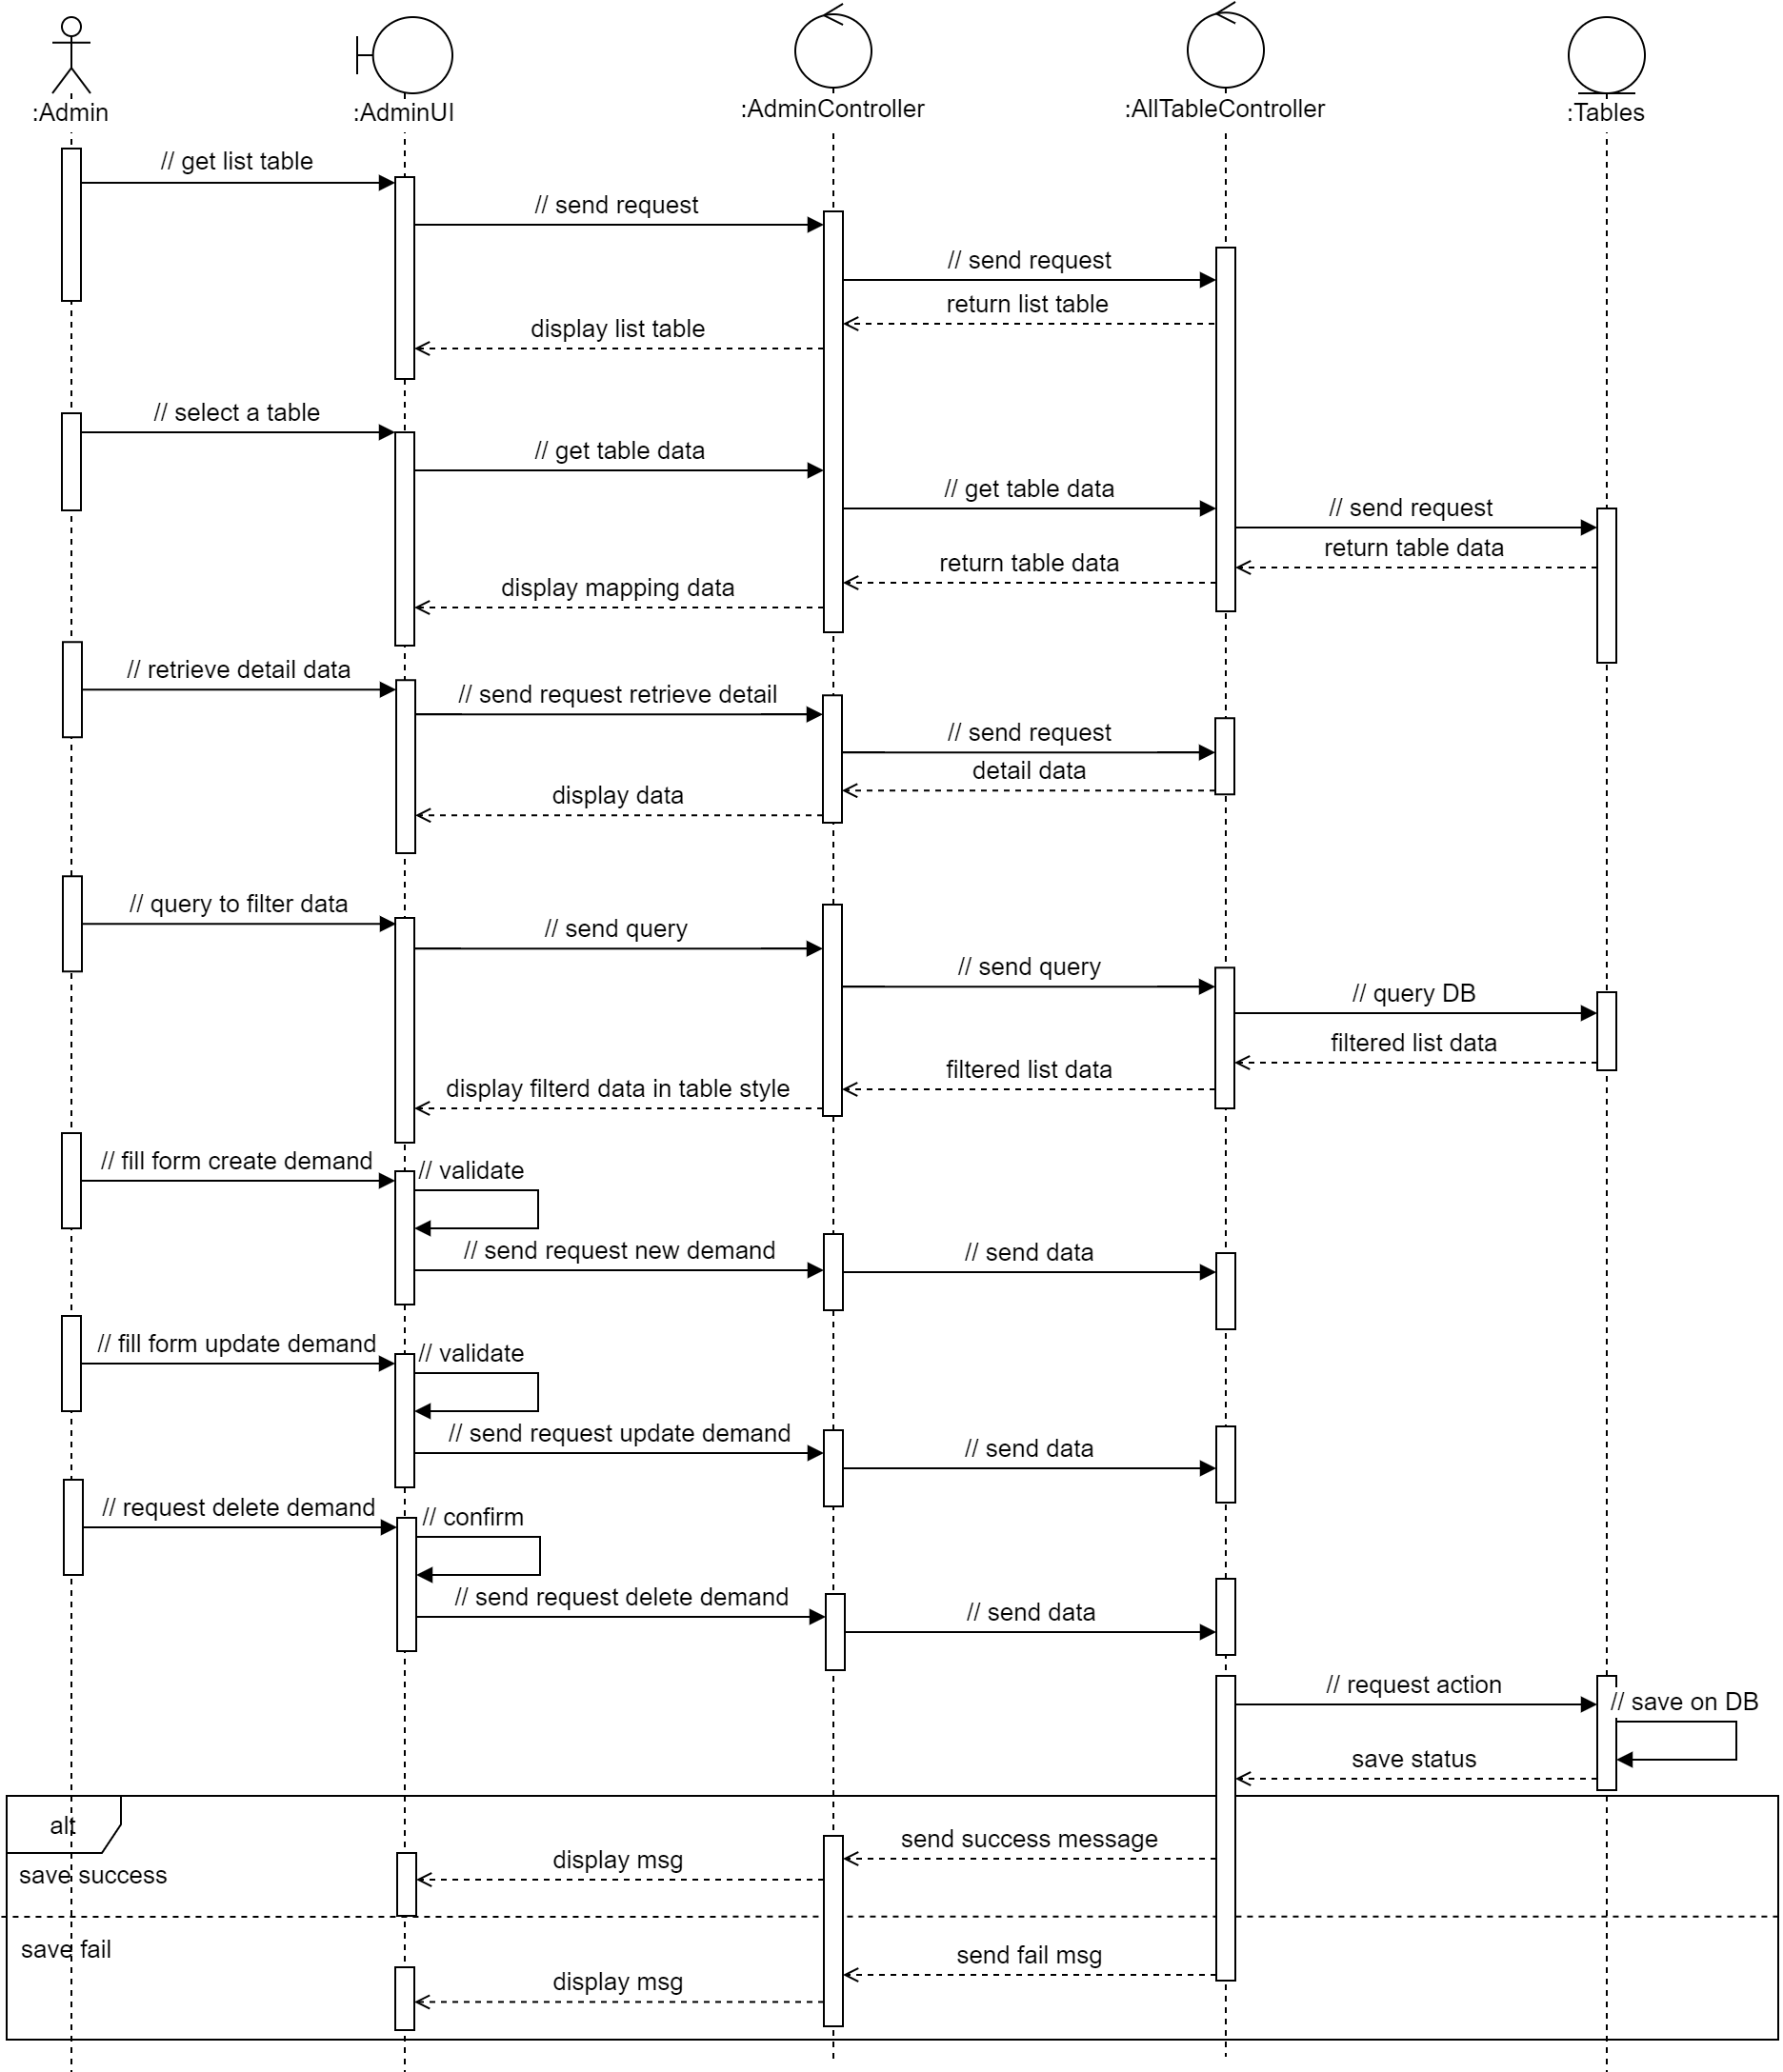
\includegraphics[width=\linewidth]{./img/uc16-19.png}
	\caption{\label{tab:seq-uc11}Biểu đồ tuần tự - Các ca sử dụng quản lý của Quản trị viên}
\end{figure}
Hình \ref{tab:seq-uc11} mô tả quá trình quản lý của Quản trị viên như sau:
\begin{itemize}
    \item Quản trị viên gửi yêu cầu lấy danh sách bảng lên máy chủ, máy chủ tiếp nhận yêu cầu, trả về danh sách bảng cho quản trị viên.
    \item Quản trị viên gửi yêu cầu lấy dữ liệu của bảng lên máy chủ, máy chủ tiếp nhận yêu cầu, trả về dữ liệu bảng mà quản trị viên đã chọn.
    \item Quản trị viên gửi yêu cầu lấy danh sách dữ liệu lên máy chủ, yêu cầu này có thể bao gồm từ khóa để tìm kiếm hoặc tùy chọn lọc.
    \item Máy chủ kiểm tra yêu cầu, nếu hợp lệ, sẽ tùy thuộc vào yêu cầu có thêm từ khóa tìm kiếm hay tùy chọn lọc hay không mà máy chủ thực hiện truy vấn phù hợp trong cơ sở dữ liệu để lấy danh sách dữ liệu thỏa mãn yêu cầu để trả về cho quản trị viên.
    \item Quản trị viên chọn tạo hoặc cập nhật dữ liệu, sẽ xuất hiện biểu mẫu cho quản trị viên nhập thông tin và ấn gửi, nếu thông tin được nhập hợp lệ sẽ gửi yêu cầu lên máy chủ, nếu không hợp lệ sẽ thông báo cho quản trị viên biết để sửa.
    \item Máy chủ tiếp nhận yêu cầu tạo hoặc cập nhật dữ liệu, nếu yêu cầu hợp lệ sẽ lưu lại thông tin vào trong cơ sở dữ liệu và thông báo cho quản trị viên yêu cầu thành công, nếu không hợp lệ thông báo cho quản trị viên biết yêu cầu thất bại.
    \item Quản trị viên chọn xóa dữ liệu và ấn xác nhận sẽ gửi yêu cầu xóa dữ liệu lên máy chủ.
    \item Máy chủ nhận được yêu cầu xóa dữ liệu, thực hiện yêu cầu, nếu thành công sẽ xóa dữ liệu trong cơ sở dữ liệu và thông báo cho quản trị viên xóa dữ liệu thành công, nếu xóa thất bại sẽ thông báo cho quản trị viên xóa dữ liệu thất bại.
\end{itemize}

\subsection{Xác minh tài khoản mới}
\begin{figure}[H]
	\centering
	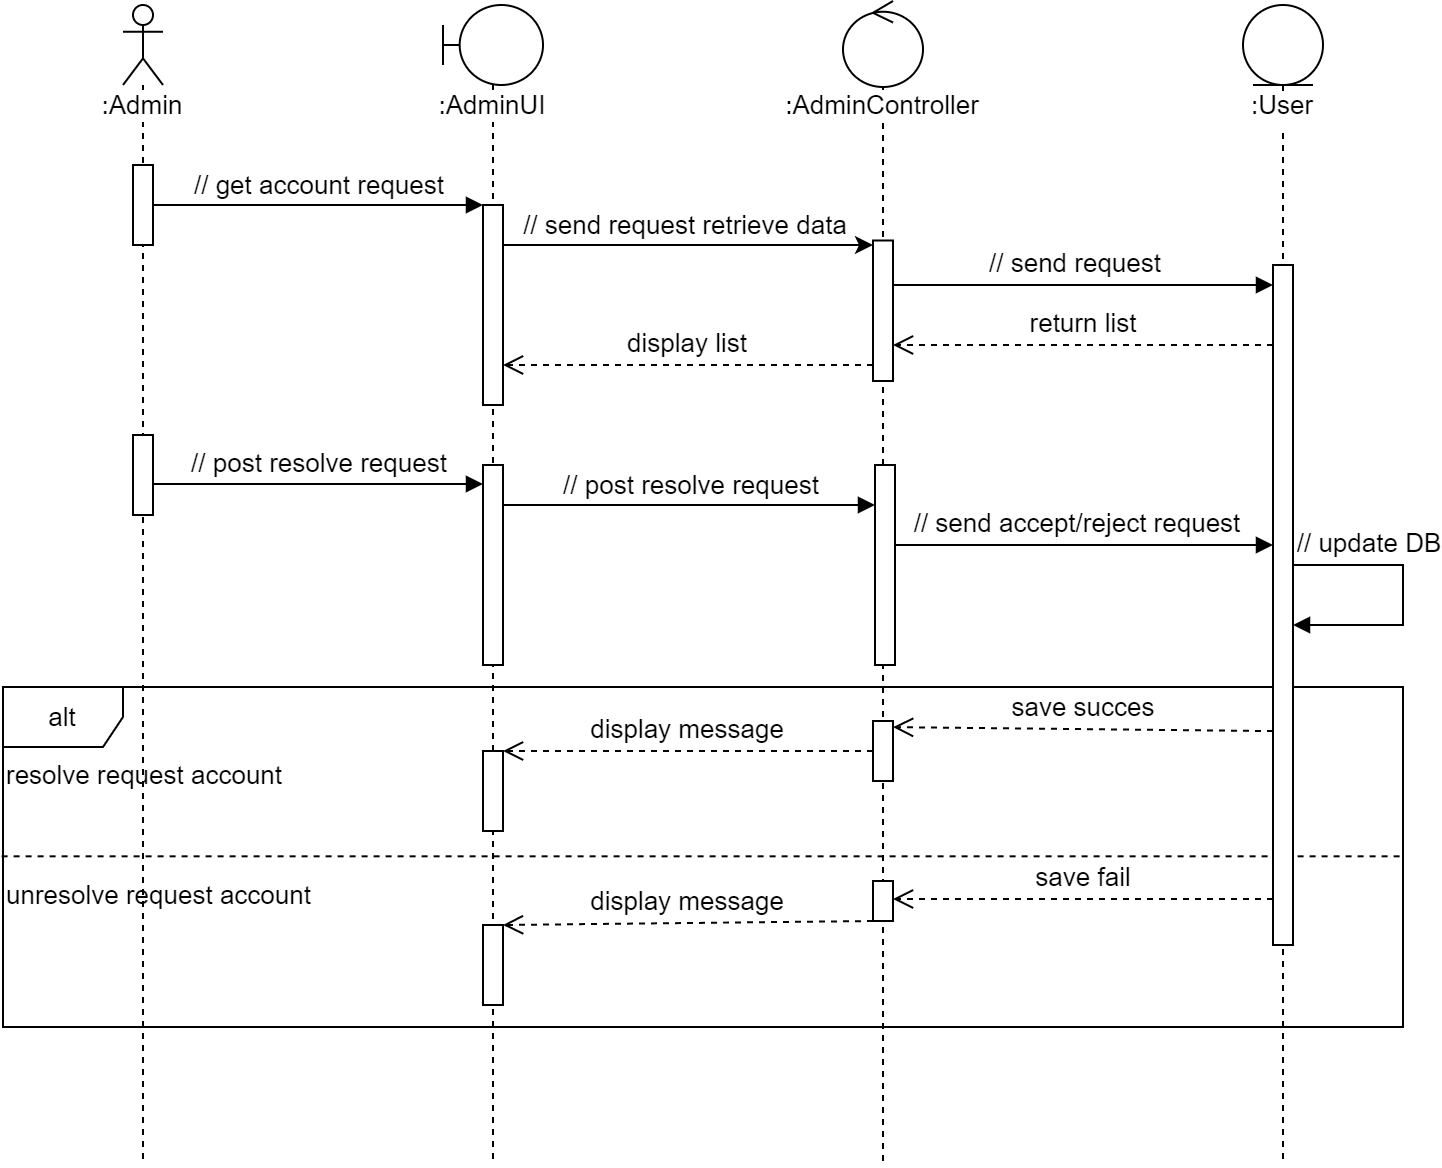
\includegraphics[width=\linewidth]{./img/uc20.png}
	\caption{\label{tab:seq-uc12}Biểu đồ tuần tự - Ca sử dụng Xác minh tài khoản mới}
\end{figure}
Hình \ref{tab:seq-uc12} mô tả quá trình xác minh tài khoản mới như sau:
\begin{itemize}
    \item Quản trị viên gửi yêu cầu lấy danh sách các tài khoản cần xác minh, máy chủ tiếp nhận yêu cầu, trả về danh sách các tài khoản cần xác minh cho quản trị viên.
    \item Quản trị viên chọn tài khoản cần xác minh, thực hiện hành động với tài khoản đó và gửi yêu cầu lên máy chủ. Máy chủ tiếp nhận yêu cầu, thực hiện lưu thông tin vào cơ sở dữ liệu tùy thuộc vào hành động quản trị viên đã chọn. Nếu thành công, thông báo cho quản trị viên biết yêu cầu thành công, nếu thất bại sẽ thông báo yêu cầu thất bại.
\end{itemize}

Tài khoản do khách tạo có vai trò mặc định là chưa xác định. Để các tài khoản đó có thể truy cập vào hệ thống và thực hiện các chức năng như của người dùng, quản trị viên cần cấp cho tài khoản quyền người dùng. Hay nói cách khác, bằng cách cấp tài khoản các vai trò tương ứng: người dùng, quản trị viên, khi đăng nhập vào hệ thống sẽ có các chức năng tương tự.

\subsection{Tạo mới tài khoản}
\begin{figure}[H]
	\centering
	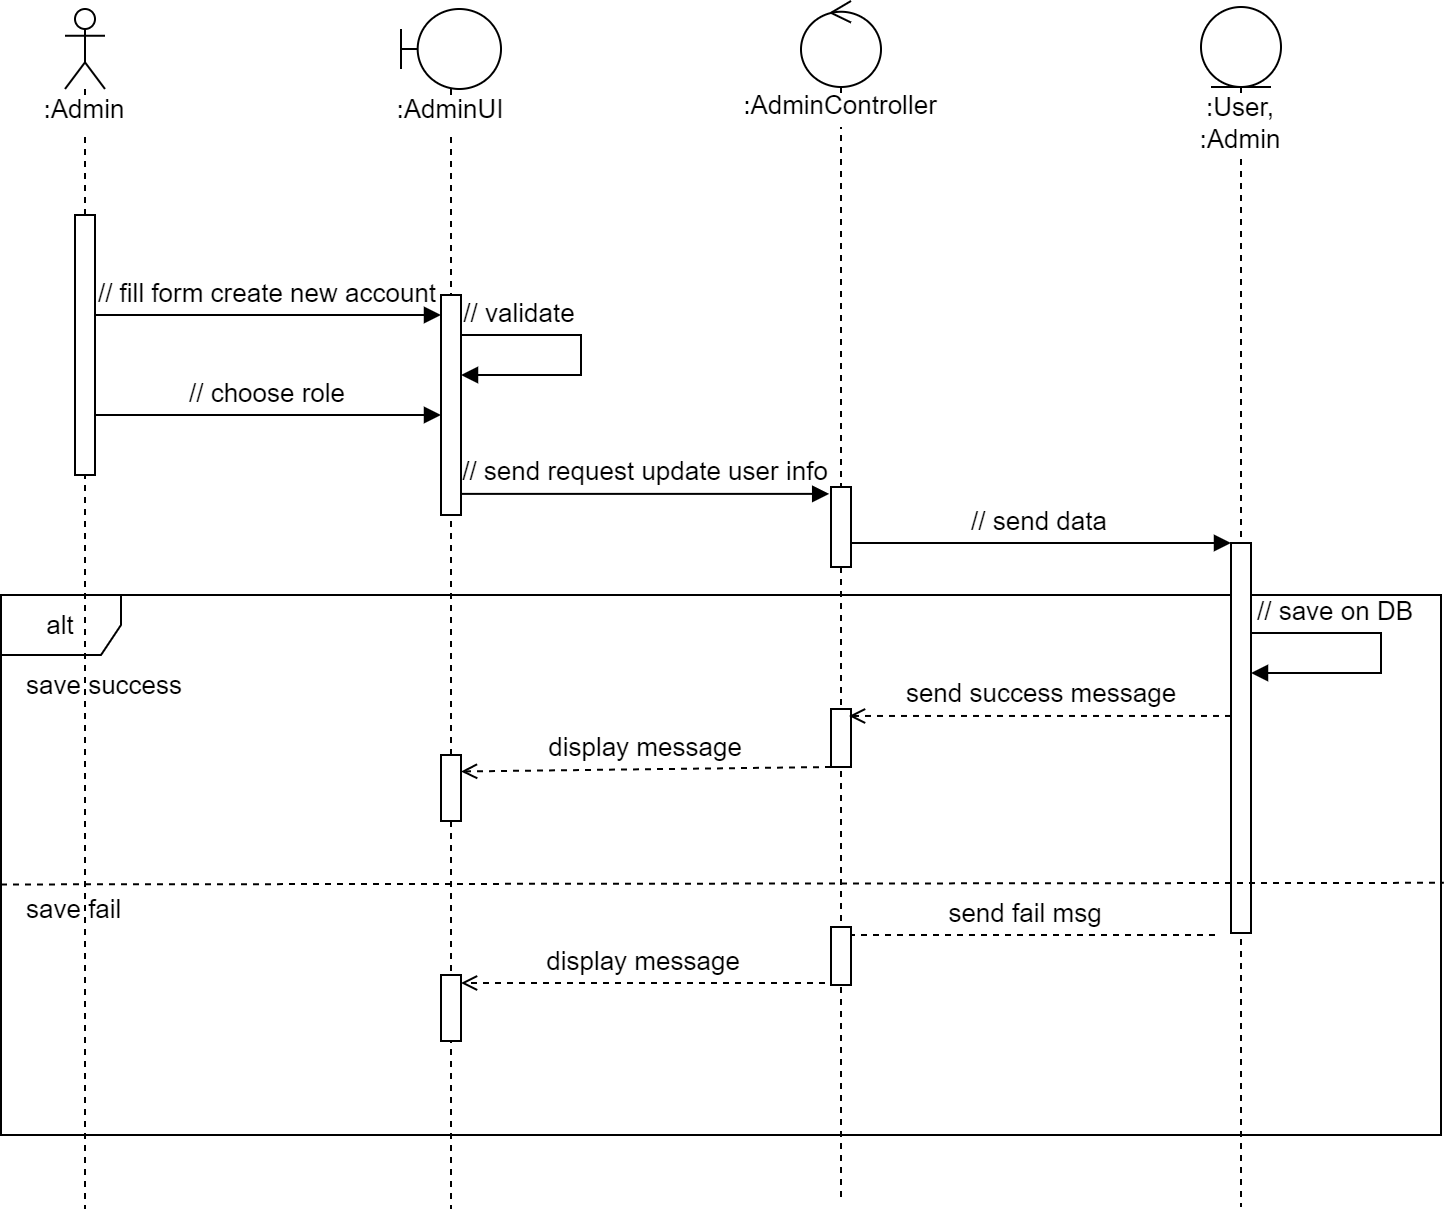
\includegraphics[width=\linewidth]{./img/uc21.png}
	\caption{\label{tab:seq-uc13}Biểu đồ tuần tự - Ca sử dụng Tạo mới tài khoản}
\end{figure}
Hình \ref{tab:seq-uc13} mô tả quá trình tạo mới tài khoản như sau:
\begin{itemize}
    \item Quản trị viên nhập thông tin tài khoản vào biểu mẫu và tạo, nếu biểu mẫu không hợp lệ sẽ thông báo cho quản trị viên biết để sửa, nếu hợp lệ sẽ gửi biểu mẫu lên máy chủ.
    \item Máy chủ nhận được yêu cầu tạo tài khoản, kiểm tra yêu cầu và biểu mẫu, nếu hợp lệ sẽ lưu lại thông tin tài khoản vào cơ sở dữ liệu và thông báo cho quản trị viên biết tạo tài khoản thành công, nếu không hợp lệ sẽ thông báo cho quản trị viên biết lý do tạo tài khoản thất bại.
\end{itemize}

Quản trị viên cũng có khả năng tạo tài khoản cho người dùng hoặc quản trị viên mới. Tài khoản được quản trị viên tạo sẽ không cần phải thông qua bước xác minh.

\end{document}